%% bare_jrnl.tex
%% V1.4b
%% 2015/08/26
%% by Michael Shell
%% see http://www.michaelshell.org/
%% for current contact information.
%%
%% This is a skeleton file demonstrating the use of IEEEtran.cls
%% (requires IEEEtran.cls version 1.8b or later) with an IEEE
%% journal paper.
%%
%% Support sites:
%% http://www.michaelshell.org/tex/ieeetran/
%% http://www.ctan.org/pkg/ieeetran
%% and
%% http://www.ieee.org/

%%*************************************************************************
%% Legal Notice:
%% This code is offered as-is without any warranty either expressed or
%% implied; without even the implied warranty of MERCHANTABILITY or
%% FITNESS FOR A PARTICULAR PURPOSE! 
%% User assumes all risk.
%% In no event shall the IEEE or any contributor to this code be liable for
%% any damages or losses, including, but not limited to, incidental,
%% consequential, or any other damages, resulting from the use or misuse
%% of any information contained here.
%%
%% All comments are the opinions of their respective authors and are not
%% necessarily endorsed by the IEEE.
%%
%% This work is distributed under the LaTeX Project Public License (LPPL)
%% ( http://www.latex-project.org/ ) version 1.3, and may be freely used,
%% distributed and modified. A copy of the LPPL, version 1.3, is included
%% in the base LaTeX documentation of all distributions of LaTeX released
%% 2003/12/01 or later.
%% Retain all contribution notices and credits.
%% ** Modified files should be clearly indicated as such, including  **
%% ** renaming them and changing author support contact information. **
%%*************************************************************************


% *** Authors should verify (and, if needed, correct) their LaTeX system  ***
% *** with the testflow diagnostic prior to trusting their LaTeX platform ***
% *** with production work. The IEEE's font choices and paper sizes can   ***
% *** trigger bugs that do not appear when using other class files.       ***                          ***
% The testflow support page is at:
% http://www.michaelshell.org/tex/testflow/



\documentclass[journal]{IEEEtran}
%\usepackage{CormorantGaramond}

\usepackage{xurl}
\usepackage{graphicx}
\usepackage[bookmarksdepth=subsubsection]{hyperref}
\usepackage{xr-hyper}

\externaldocument[main-]{sn-article}

\usepackage{booktabs, multirow, caption}
\usepackage{siunitx}
% -- global siunitx settings for "mean ± std" --------------------
\sisetup{
  detect-all,
  separate-uncertainty,
  table-number-alignment = center,
  table-figures-integer  = 3,
  table-figures-decimal  = 3,
  table-figures-uncertainty = 2,
  table-space-text-post = *,
  uncertainty-separator = {\,\text{±}\,}
}



%\usepackage{ebgaramond}
%\usepackage{palatino}

\usepackage{lettrine}
\usepackage{hhline}
\usepackage{adjustbox}
\usepackage{graphicx}
\usepackage{xcolor}
\usepackage{float}
\graphicspath{images/}
\usepackage{mathrsfs}
\usepackage{caption}
\usepackage{cite}
\usepackage{subcaption}
\usepackage{comment}
\usepackage[linesnumbered,ruled,vlined]{algorithm2e}
\usepackage{adjustbox}    
\usepackage{pdfpages}
%\usepackage{cuted}
%\usepackage[ruled,vlined]{algorithm2e}
\usepackage{tabularx}
\usepackage{tikz}
\usetikzlibrary{shapes.arrows, positioning}
% prooftrees unused
\usepackage{amsthm}
\newtheorem{claim}{Claim}
\usepackage{algpseudocode}
%\usepackage{algorithm2e}
%\usepackage{algorithm}
%\usepackage{algorithmicx}
%\usepackage{algcompatible}
\usepackage{array}
\renewcommand{\arraystretch}{1.2}

\setlength{\arrayrulewidth}{0.3mm}
\setlength{\tabcolsep}{2pt}
\renewcommand{\arraystretch}{1.0}

\usepackage[shortlabels]{enumitem}
%\usepackage{newpxtext}
\usepackage{booktabs}
%\usepackage{hyperref}
% \usepackage{booktabs}
\usepackage{threeparttable}
\usepackage{threeparttablex}
\usepackage{multirow}
\usepackage{longtable}
\usepackage{siunitx}
\sisetup{detect-weight=true,table-number-alignment=center}
\usepackage{siunitx}

\usepackage{amsmath}
\usepackage{amssymb}
\usepackage{stackrel}
\usepackage{makecell}

\newcolumntype{Y}{>{\centering\arraybackslash}X}
\usepackage{mathtools}
%\usepackage{sfmath}
\usepackage{pgfplots}
\pgfplotsset{compat=1.17}
\usepackage{subcaption}
\usepackage{caption}
\usepackage{amsmath}
\usepackage{lipsum}
 
\usepackage{amsthm}
\newtheorem{theorem}{Theorem}
\newtheorem{remark}{Remark}
\newtheorem{lemma}{Lemma}
\theoremstyle{definition}
\newtheorem{definition}{Definition}[section]
% \newtheorem{lemma}{Lemma}
\newtheorem{corollary}{Corollary}
\newcommand{\negl}{\mathsf{negl}}

\newtheoremstyle{game}%
  {3pt}% Space above
  {3pt}% Space below
  {\itshape}% Body font
  {}% Indent amount
  {\bfseries}% Theorem head font
  {.}% Punctuation after theorem head
  { }% Space after theorem head
  {}% Theorem head spec
\theoremstyle{game}
\newtheorem{game}{Game}[section]
\usepackage{setspace}
\usepackage[a4paper, total={7.3in, 10.2in}]{geometry}
\renewcommand{\arraystretch}{1.5}


\usepackage[T1]{fontenc}
%\usepackage{lmodern}
\usepackage{microtype}
\usepackage{booktabs, multirow, tabularx}
\usepackage{subcaption}
\usepackage[capitalise]{cleveref}
%\onehalfspacing
\hypersetup{
    colorlinks=true,
    linkcolor=blue,
    urlcolor=blue,
    citecolor=blue
}

% Custom command for consistent technical term formatting
\newcommand{\techterm}[1]{\textbf{\textit{#1}}}



\ifCLASSINFOpdf
  % \usepackage[pdftex]{graphicx}
  % declare the path(s) where your graphic files are
  % \graphicspath{{../pdf/}{../jpeg/}}
  % and their extensions so you won't have to specify these with
  % every instance of \includegraphics
  % \DeclareGraphicsExtensions{.pdf,.jpeg,.png}
\else
  % or other class option (dvipsone, dvipdf, if not using dvips). graphicx
  % will default to the driver specified in the system graphics.cfg if no
  % driver is specified.
  % \usepackage[dvips]{graphicx}
  % declare the path(s) where your graphic files are
  % \graphicspath{{../eps/}}
  % and their extensions so you won't have to specify these with
  % every instance of \includegraphics
  % \DeclareGraphicsExtensions{.eps}
\fi
% graphicx was written by David http://www.ctan.org/pkg/algorithmicx





\hyphenation{op-tical net-works semi-conduc-tor steg-a-nog-ra-phy}


\begin{document}
%
% paper title
% Titles are generally capitalized except for words such as a, an, and, as,
% at, but, by, for, in, nor, of, on, or, the, to and up, which are usually
% not capitalized unless they are the first or last word of the title.
% Linebreaks \\ can be used within to get better formatting as desired.
% Do not put math or special symbols in the title.
\title{Supplementary Material for\\
``Cover-Parameterised Multichannel Hybrid Steganography: Compositional Security, Detectability, and Robustness''}
%
%
% 
%








% The paper headers
\markboth{SUPPLEMENTARY MATERIAL}{SUPPLEMENTARY MATERIAL}%





% make the title area
\author{}
\maketitle

% As a general rule, do not put math, special symbols or citations
% in the abstract or keywords.
\noindent
This supplementary material provides the detailed theoretical constructions, security games and proofs, experimental methodology, ablation studies, and additional results supporting the main manuscript. References prefixed by ``main-'' refer to sections, equations, figures, tables, claims, and theorems in the main paper.








\IEEEpeerreviewmaketitle




\appendices




\section{Receiver-Reproducible Masking and Image-Domain Construction}
\label{sec:qim-construction}
\subsection{Receiver-reproducible masking construction}\label{subsec:qim-mask-theory}
The executable reference \texttt{cpm-epoch-v2} uses one binary mask in the
model, sender, receiver and correctness argument. The component experiments
using an original-feature-conditioned mask are identified separately in
Appendix~\ref{sec:reproducibility}; their results are not transferred to
this received-field construction.

For exact byte strings $\gamma_{1,e},\gamma_{2,e}$, define public streams
\begin{align}\label{supp-eq:qim-parameter-extraction}
G_{j,\ell_e}(\gamma_{j,e})&=
 \mathsf{Trunc}_{\ell_e}\!\left(\mathsf{SHAKE256}
 (\mathsf{Encode}(\texttt{cp}j,\gamma_{j,e}))\right),\nonumber\\
P_{\mathsf{params},e}&=G_{1,\ell_e}(\gamma_{1,e})\oplus G_{2,\ell_e}(\gamma_{2,e}).
\end{align}
The concrete encoding labels the domain and object fields and preserves
their exact bytes. These mappings are public; arbitrary deterministic maps
would preserve the uniform-mask cancellation argument, so their output is
not counted as additional secret entropy.

\paragraph{Receiver-available context.}
\begin{equation}\label{supp-eq:qim-mask-context}
\eta_e=\mathsf{Encode}(v,\mathsf{sid},H_e,n_{a,e},n_{b,e},n_{c,e},\ell_e,\mathsf{codec}).
\end{equation}
Version, session identifier, epoch/header, three nonces, payload length and
codec are available from the agreed session and received frames. All are
covered by the epoch tag. Neither a hash of the original image nor
$\Phi(o_e)=\Phi(s_e)$ is required. Thus context reconstruction is exact for
an unaltered canonically parsed authenticated epoch. Suppressed or altered
context is rejected. Unique session/epoch use is essential to prevent mask reuse.

\paragraph{Domain-separated keys and streams.}
Purpose key $K_L$ is HMAC-SHA256 under the master secret over
\texttt{derive} and the labelled encoding of version, session, and purpose.
For mask blocks $r=0,1,\ldots$, concatenate
\begin{equation}\label{supp-eq:qim-mask-seed}
\mathsf{HMAC}_{K_{\mathsf{mask}}}
 (\texttt{payload-mask}\parallel\eta_e\parallel\mathsf{uint64}(r))
\end{equation}
and truncate to $\ell_e$ bits to obtain $\rho_{\mathsf{dit},e}$.
The most significant $\ell_e$ bits of the packed bytes are used; unused
low bits of the last byte are zero. Define
\begin{align}\label{supp-eq:qim-cover-parameter-bits}
\mu_e&=P_{\mathsf{params},e}\oplus\rho_{\mathsf{dit},e},\\
\label{supp-eq:qim-theoretical-masked-payload}
b_e&=m_e\oplus\mu_e.
\end{align}
The payload mask is binary PRF/XOR masking, without a scalar
quantisation step. QIM-inspired
modulation belongs to the subsequent sender-side cost construction.

\paragraph{Embedding and blind extraction.}
\begin{equation}\label{supp-eq:qim-theoretical-embedding}
s_e=\mathsf{STC.Enc}(o_e,b_e;\rho_e^-,\rho_e^+,\mathsf{seed}(K_{\mathsf{emb}},\eta_e)).
\end{equation}
The sender computes directional costs from image features using a distinct
$K_{\mathsf{cost}}$. The native backend expects minus costs followed by plus
costs; the complete-epoch adapter follows that argument order. For this backend,
the receiver needs only the stego-image and context-derived seed, not
the original image, cost map, or sender-generated mask:
\begin{align}\label{supp-eq:qim-extracted-payload}
\widehat b_e&=\mathsf{STC.Dec}(s_e;\mathsf{seed}(K_{\mathsf{emb}},\eta_e)),\\
\label{supp-eq:qim-theoretical-unmasking}
\widehat m_e&=\widehat b_e\oplus\mu_e.
\end{align}
The 31-bit pySTC permutation seed is a coding parameter, not the source of
payload confidentiality. No key-recovery strength of 256 bits is attributed
to that seed. The keyed payload-mask stream has a separate 256-bit purpose key.
Byte padding and the backend's 32-bit length header are reported separately
from application payload bits; the header occupies 64 host pixels.

\paragraph{Correctness and masking scope.}
\begin{equation}\label{supp-eq:qim-mask-correctness}
\widehat b_e=b_e\ \Longrightarrow\ \widehat m_e=m_e,\qquad
\Pr[\mathsf{Accept}_e\wedge\widehat m_e\ne m_e]\le\delta_{\mathsf{dec}}.
\end{equation}
For the adopted lossless-byte context, parameter/context disagreement is
zero after valid authentication; actual embedding/decoding failures remain
in $\delta_{\mathsf{dec}}$. The sender preflight is a measured rejection
condition, not a reason to omit failed attempts from the denominator.

For every permitted PPT distinguisher, including the public parameter
strings, context, and allowed prior/oracle history, write $Z_e=(P_{\mathsf{params},e},\eta_e,V)$ and require
\begin{align}\label{supp-eq:qim-mask-pseudorandomness}
\left|\Pr[\mathcal D(\mu_e,Z_e)=1]
-\Pr[\mathcal D(U_{\ell_e},Z_e)=1]\right|
\le\varepsilon_{\mathsf{param}}.
\end{align}
After purpose-key replacement, this reduces to PRF stream security on
distinct block inputs: XOR by a known public stream preserves uniformity.
This is computational pseudorandomness, not a statistical TV claim and not
image indistinguishability. The sampler's separate loss is detailed below.

\subsection{QIM-Fused-CF Image-Domain Embedding}
\label{subsec:ours-qim-fused-cf}

This subsection specifies the concrete image-domain encoder used
to generate the stego-object on $C_3$. It instantiates
$\mathsf{Enc}/\mathsf{Dec}$ in
\eqref{supp-eq:qim-theoretical-embedding} and
\eqref{supp-eq:qim-extracted-payload}; it does not redefine the
masking operation of
Section~\ref{main-Hybrid_stego_model}. See also
Section~\ref{main-Embedding methods} of the main manuscript.

Let
$\mathbf{o}_e\in\{0,\ldots,255\}^{H\times W}$ denote the
grayscale cover image for epoch $e$, where $N=HW$ and pixels are
indexed by $i\in\{1,\ldots,N\}$. For a target payload rate
$\alpha$ bits per pixel, the embedded payload length is
\begin{equation}
L_e
=
\operatorname{round}(\alpha N).
\label{eq:qim_payload_length}
\end{equation}
Here $L_e$ is the requested application-bit count, so $\ell_e=L_e$
when the message is generated at the target rate. Byte padding and the
native STC length header are additional framing, as detailed in
Section~\ref{subsec:repro-stc}. This local notation is distinct from the
transcript byte length in the main complexity analysis and epoch latency
in the scheduling study.
Let $\mathbf m_e\in\{0,1\}^{\ell_e}$ be the application bitstream.
The complete-epoch image adapter first applies the single mask above:
\begin{equation}\label{eq:qim_masked_payload}
\mathbf b_e=\mathbf m_e\oplus G_{1,\ell_e}(\gamma_{1,e})
 \oplus G_{2,\ell_e}(\gamma_{2,e})\oplus\rho_{\mathsf{dit},e}.
\end{equation}
The receiver regenerates the payload stream by
\begin{equation}\label{eq:qim_dither_stream}
\rho_{\mathsf{dit},e}=\mathsf{Stream}_{K_{\mathsf{mask}}}
(\texttt{payload-mask},\eta_e,\ell_e).
\end{equation}
Original-image features remain sender-side cost inputs. The cost-modulation
map $u_i=\mathsf{CostDither}(K_{\mathsf{cost}},\eta_e,\Psi(o_e),i)$ uses a
separate purpose key and is not the payload mask. STC extraction requires
the context-derived permutation seed, not the cost map or original image.
The component image results use the original-feature mask/keying path.
Independent receiver checks and the matched HSMNet comparison evaluate the
received-field construction (main Sections~\ref{main-subsec:revised-pilot}
and \ref{main-subsec:hsmnet-comparison}).

For each pixel $i$, two directional base distortion maps are computed. The first is an S-UNIWARD-type spatial cost, denoted by $\rho_{i,\mathsf{S}}^{+}$ and $\rho_{i,\mathsf{S}}^{-}$, obtained from directional wavelet residuals. The second is a MiPOD-inspired statistical cost, denoted by $\rho_{i,\mathsf{M}}^{+}$ and $\rho_{i,\mathsf{M}}^{-}$, obtained from local residual variance and detectability-oriented statistical proxies. To combine the directional residual sensitivity of S-UNIWARD with the statistical detectability principle of MiPOD, QIM-Fused-CF uses a log-domain fused base cost:
\begin{align}
    \rho_{i,\mathsf{base}}^{+}
    &=
    \exp\!\left(
    \lambda \log(\rho_{i,\mathsf{S}}^{+}+\epsilon)
    +(1-\lambda)\log(\rho_{i,\mathsf{M}}^{+}+\epsilon)
    \right),
    \label{eq:qim_base_cost_plus}
    \\
    \rho_{i,\mathsf{base}}^{-}
    &=
    \exp\!\left(
    \lambda \log(\rho_{i,\mathsf{S}}^{-}+\epsilon)
    +(1-\lambda)\log(\rho_{i,\mathsf{M}}^{-}+\epsilon)
    \right),
    \label{eq:qim_base_cost_minus}
\end{align}
where $\epsilon>0$ prevents numerical instability. Here $\lambda$ is the fusion weight, distinct from the formal security
parameter. In the fixed configuration, $\lambda=0.75$, making the fused map S-UNIWARD-dominant while retaining a MiPOD-derived statistical correction.

The cover-complexity map $\Psi(\mathbf{o})$ is constructed from complementary local descriptors, including directional residual energy, SRM-like high-pass residual responses, fuzzy edge confidence, sharpened residual energy, local variance, and a local entropy proxy. The resulting value $\psi_i(\mathbf{o})\in[0,1]$ is larger in complex, textured, or edge-rich regions, where embedding changes are typically less visually and statistically exposed. A keyed dither map $u_i\in[0,1]$ is also generated from $\mathsf{CostDither}(K_{\mathsf{cost}},\eta_e,\Psi(\mathbf{o}))$. The fused base cost is then modulated by a conservative QIM-style factor
\begin{equation}
\begin{aligned}
\widetilde{g}_i
&\triangleq
\Bigl[
  1+\beta_{\mathsf{s}}\bigl(1-\psi_i(\mathbf{o})\bigr)
  -\beta_{\mathsf{t}}\psi_i(\mathbf{o})
\Bigr]
\\[-1mm]
&\qquad{}\times
\Bigl[
  1+\beta_{\mathsf{d}}
  \bigl(u_i-\tfrac{1}{2}\bigr)
\Bigr],
\\[1mm]
g_i
&=
\operatorname{clip}_{[g_{\min},g_{\max}]}
\left(
\frac{\widetilde{g}_i}
     {\operatorname{GM}_{j=1}^{N}
      \bigl(\widetilde{g}_j\bigr)}
\right).
\end{aligned}
\label{eq:qim_modulation_factor}
\end{equation}




where $\operatorname{GM}(\cdot)$ denotes geometric-mean normalization. Before clipping, this normalization gives the multipliers unit geometric
mean; clipping can change that mean. The operation changes relative
embedding preferences without guaranteeing an exactly preserved final scale. In the final setting, $\beta_{\mathsf{t}}=0.08$, $\beta_{\mathsf{s}}=0.08$, $\beta_{\mathsf{d}}=0.01$, $g_{\min}=0.85$, and $g_{\max}=1.20$. The QIM-modulated directional costs are
\begin{equation}
    \rho_{i,\mathsf{qim}}^{\pm}
    =
    \rho_{i,\mathsf{base}}^{\pm} g_i .
    \label{eq:qim_modulated_cost}
\end{equation}

A second cover-complexity refinement is applied to encourage complexity-first embedding while avoiding overly sparse or isolated modification patterns. Let $\mathcal{R}_i\in\{0,1\}$ denote the SLIC-guided selected-region mask, where $\mathcal{R}_i=1$ identifies pixels belonging to sufficiently complex regions. Pixels outside selected regions are penalized by a mild factor $\kappa\geq 1$. A fine-grained complexity multiplier is defined as
\begin{equation}
    h_i
    =
    \operatorname{clip}_{[h_{\min},h_{\max}]}
    \left(
    1+\eta_{\mathsf{s}}(1-\psi_i(\mathbf{o}))
    -\eta_{\mathsf{t}}\psi_i(\mathbf{o})
    \right),
    \label{eq:qim_fine_complexity_factor}
\end{equation}
where $\eta_{\mathsf{t}}=0.03$ and $\eta_{\mathsf{s}}=0.03$ in the final configuration. The region-refined costs are
\begin{equation}
    \widetilde{\rho}_{i}^{\pm}
    =
    \rho_{i,\mathsf{qim}}^{\pm}
    h_i
    \left[
    \mathcal{R}_i+\kappa(1-\mathcal{R}_i)
    \right],
    \label{eq:qim_region_refined_cost}
\end{equation}
with $\kappa=1.02$. To reduce isolated selection-channel spikes, a local spreading operation is then applied:
\begin{equation}
    \rho_{i,\mathsf{ours}}^{\pm}
    =
    (1-\mu)\widetilde{\rho}_{i}^{\pm}
    +
    \mu\,
    \mathcal{A}_{3\times3}\!\left(\widetilde{\boldsymbol{\rho}}^{\pm}\right)_i,
    \label{eq:qim_spread_cost}
\end{equation}
where $\mathcal{A}_{3\times3}(\cdot)$ is a local mean filter and $\mu=0.05$. Boundary constraints are enforced using a wet cost $C_{\mathsf{wet}}$:
\begin{equation}
    \rho_{i,\mathsf{ours}}^{+}=C_{\mathsf{wet}}
    \quad\text{if } o_i=255,
    \qquad
    \rho_{i,\mathsf{ours}}^{-}=C_{\mathsf{wet}}
    \quad\text{if } o_i=0.
    \label{eq:qim_wet_cost}
\end{equation}
In the final configuration, explicit direction-adaptive polarity modulation is disabled; directional asymmetry is therefore induced only by the fused base costs and wet-cost boundary constraints.

The final embedding is performed using syndrome-trellis coding (STC). The encoder supplies directional costs for intended ternary changes
$\Delta_i\in\{-1,0,+1\}$. The following additive objective describes
that coding interface, rather than a guaranteed bound on every pixel
of the native output. The stego image $\mathbf{s}$ targets the STC
payload constraint for $\mathbf{b}_{\mathsf{qim}}$ while minimising
the supplied additive directional distortion
\begin{equation}
    D(\mathbf{o},\mathbf{s})
    =
    \sum_{i=1}^{N} d_i(\Delta_i),
    \label{eq:qim_distortion}
\end{equation}
where
\begin{equation}
    d_i(\Delta_i)
    =
    \begin{cases}
    0, & \Delta_i=0,\\
    \rho_{i,\mathsf{ours}}^{+}, & \Delta_i=+1,\\
    \rho_{i,\mathsf{ours}}^{-}, & \Delta_i=-1.
    \end{cases}
    \label{eq:qim_directional_distortion}
\end{equation}

The resulting image-domain embedding variant is denoted \textbf{QIM-Fused-CF}.
Here $\mathbf b_{\mathsf{qim}}$ denotes the binary PRF/XOR-masked
payload $b_e$. QIM-inspired modulation applies to the sender cost map.
The encoder combines fused costs, complexity/region refinement, cost
spreading and STC. Native outputs are audited as produced: the two-level
change disclosed in Section~\ref{sec:revision-details} is retained.
No post-stego adversarial perturbation is applied.


\section{Key-Provisioning Considerations}
\label{subsec:key-provisioning}

The formal model assumes a pre-established master secret
$V_{\mathsf{pri}}$ and does not depend on a particular
key-establishment mechanism. In practice, such a secret may be
provisioned through secure hardware, an authenticated out-of-band
procedure, or deployment-specific techniques such as
PUF-assisted key derivation or wireless reciprocity-based secret
key generation
\cite{holcomb2010power,delvaux2014helper,ye2009infotheoretic,xu2021key}.
These mechanisms impose their own assumptions and security
requirements and are therefore treated as deployment options
rather than components of the CPM security proof.

\section{Detailed Security Assumptions and Scope}
\label{subsec:security_assumptions}

This subsection expands Assumptions~A1--A6 stated in the main
manuscript. It does not introduce additional security premises;
rather, it makes explicit the probability spaces, implementation
conditions, and limitations required by the formal games in
Section~\ref{main-subsec:formal}, the hybrid-composition result in
Theorem~\ref{main-thm:composition}, the synchronisation analysis in
Lemma~\ref{main-lem:resync}, and Claims~\ref{main-Claim1}--
\ref{main-Claim4}. Throughout, $\lambda$ is the security parameter,
$\mathcal{A}$ is a probabilistic polynomial-time adversary, and
$\mathsf{View}_{\mathcal A}$ contains all public parameters,
protocol frames, metadata, timing observations, and oracle answers
made available in the corresponding game.
\subsection{Assumptions}

\subsubsection{A1: Key establishment and domain separation}\label{supp-assump:a1}
The master secret has at least 256 bits of effective key entropy, remains
secret, and is provisioned outside the network-adversary model. Purpose keys
use the exact version/session/purpose-labelled HMAC derivation in the main
protocol. The KDF/PRF premise permits replacement of the permitted family of
purpose keys by independent keys at cost $\varepsilon_{\mathsf{KDF}}$.
This cost is over the whole allowed query/session history. It follows
from the purpose-key PRF replacement, rather than from a random-oracle
key-query calculation. Provisioning, compromise, state rollback, and side
channels require separate deployment treatment \cite{nist80057pt1r5}.

\subsubsection{A2: Separate sampler, linkage, and masking premises}\label{supp-assump:a2}
The real parameter sampler is $\mathsf{Samp}(\mathsf{PRF}_{K_{\mathsf{synth}}})$;
its ideal-coins counterpart is $\mathsf{Samp}(U)$. For the stated benign joint
law conditional on public metadata, define the acceptance-gap loss
\begin{equation}\label{supp-eq:cp-ind-assumption}
\varepsilon_{\mathsf{samp}}=\sup_{\mathcal D}
\left|\Pr[\mathcal D(\mathsf{Samp}(U))=1]-
\Pr[\mathcal D(\mathcal D^{\mathsf{param}})=1]\right|.
\end{equation}
Consequently,
\begin{equation}\label{supp-eq:separate-sampler-bound}
\mathsf{Adv}^{\mathsf{CP\text{-}IND}}
\le\mathsf{Adv}^{\mathsf{PRF}}_{\mathsf{synth}}+\varepsilon_{\mathsf{samp}}.
\end{equation}
The first transition replaces keyed coins, and the second replaces the
ideal sampler by benign content. Mask pseudorandomness cannot cover either
unjustified distributional mismatch. For example, a sampler that always
outputs object A is perfectly distinguishable from benign object B even
when the independent payload mask is exactly uniform. Message independence
also does not prevent that counterexample.

After independent-key and uniform-mask replacement, the conditional
content-unlinking loss $\varepsilon_{\mathsf{unl}}$ bounds
the linked full view versus independent content marginals under the same
metadata, including visible tag distributions. Header independence and
MAC unforgeability do not by themselves prove that premise.
\begin{equation}\label{supp-eq:cp-unl-assumption}
\mathsf{Adv}^{\mathsf{CP\text{-}UNL}}(\mathcal A;H_2)\le\varepsilon_{\mathsf{unl}}.
\end{equation}
Masking is separately governed by the full public-view computational
condition in Eq.~\eqref{supp-eq:qim-mask-pseudorandomness}, denoted
\begin{equation}\label{supp-eq:param-gap}
\mathsf{Gap}_{\mathsf{mask}}\le\varepsilon_{\mathsf{param}}.
\end{equation}
The main hybrid theorem explicitly charges
$\varepsilon_{\mathsf{KDF}}$, $\varepsilon_{\mathsf{param}}$,
$\varepsilon_{\mathsf{unl}}$, sampler-PRF loss, $\varepsilon_{\mathsf{samp}}$,
carrier loss, and scheduling loss. Every bound must match the complete
history or be summed across queries. Corpus naturalness and detector
experiments probe finite instantiations; they do not prove negligible
values of these universal computational losses.

\subsubsection{A3: Embedding correctness and stego-object indistinguishability}
\label{supp-assump:a3}

The cover-modification assumption applies principally to the
stego-object carried on $C_3$. The parameter objects on $C_1$ and
$C_2$ are governed by A2 and must not be counted again in the
embedding term. For an admissible cover
$o_e\leftarrow\mathcal D_3$, payload $\mathbf b_e$, and stego-key
$K_{\mathsf{stego},e}$, let
\[
s_e
\leftarrow
\mathsf{Enc}(K_{\mathsf{stego},e},o_e,\mathbf b_e).
\]
Correctness requires
\begin{equation}
\Pr\!\left[
 \mathsf{Dec}(K_{\mathsf{stego},e},s_e)
 \neq \mathbf b_e
\right]
\leq \delta_{\mathsf{dec}}.
\label{supp-eq:dec-failure}
\end{equation}
Perfect carrier inversion would give $\delta_{\mathsf{dec}}=0$.
The correctness theorem is conditional on carrier decoding.
Experiments report extraction-failure frequencies and bit errors.
These observations do not determine a population upper bound
$\delta_{\mathsf{dec}}$ and must be distinguished from a security advantage.
If error-correcting coding is used, the event in
\eqref{supp-eq:dec-failure} is evaluated after the agreed decoding
procedure.

The carrier-replacement premise must hold over the full view at the
corresponding hybrid, including public context, auxiliary parameters,
visible tags, and permitted history. For its real-carrier and benign-carrier
views $V_{\mathsf{car}}$ and $V_{\mathsf{ben}}$, require
\begin{equation}\label{supp-eq:embedding-gap}
\sup_{\mathcal D}\left|\Pr[\mathcal D(V_{\mathsf{car}})=1]
-\Pr[\mathcal D(V_{\mathsf{ben}})=1]\right|
\le\varepsilon_{\mathsf{emb}}.
\end{equation}
The supremum is over the permitted PPT wardens. A valid statistical TV
bound on these joint views is a stronger sufficient condition. A marginal
image-distance bound alone does not establish the required conditional
transition. Computational game bounds and statistical distances remain
distinct \cite{@Hopper2002,@hopper2009provably,vonahn2003publickey}.

The empirical SRM+EC and CNN detectors estimate the performance
of particular wardens on finite samples. Their AUC, error rate,
and accuracy provide evidence about the observable embedding
footprint, but do not establish the supremum over all PPT
adversaries. For an optimal equal-prior binary test,
\[
P_e^{\star}
=\frac12\left(1-
\operatorname{TV}(\mathcal D_3,\mathsf{Law}(S_3))
\right),
\]
so the total-variation-style distinguishability is
$1-2P_e^{\star}$. A measured classifier error can therefore be
reported only as an empirical proxy unless optimality is proved.

\paragraph{Use in the main manuscript.}
A3 supports the carrier transition in Theorem~\ref{main-thm:composition}.
Message confidentiality instead follows from the joint masking premise;
acceptance of an unauthorised modified carrier is controlled by complete
transcript authentication and freshness, with decoder failure separate.

\subsubsection{A4: Complete-epoch authentication}\label{supp-assump:a4}
The separately keyed header authenticator binds the session/epoch context.
The C3-carried epoch tag binds the exact canonical transcript
\begin{align}\label{supp-eq:canonical-hmac}
\mathcal T_e&=\mathsf{Encode}_{\mathsf{epoch}}
(\eta_e,(C_1,n_{a,e},\gamma_{1,e}),\nonumber\\
&\hspace{3em}(C_2,n_{b,e},\gamma_{2,e}),(C_3,n_{c,e},s_e)),\nonumber\\
\mathsf{MAC}_e&=\mathsf{HMAC}_{K_{\mathsf{mac}}}(\texttt{epoch}\parallel\mathcal T_e).
\end{align}
The context contains all fields controlling mask and decoder reconstruction.
Each labelled value is encoded with a two-byte label length and eight-byte
value length, both big-endian. Ambiguous fields, unexpected versions/codecs,
and duplicate JSON keys are rejected by the reference parser.
EUF-CMA security bounds new-message tag forgeries
\cite{bellare1996keying,rfc2104}; persistent freshness state rejects verbatim
replay. The PRF privacy of visible tags, if needed for unlinkability, is a
separate premise. The receiver verifies the full epoch before image decoding
or committing freshness state; C1/C2 content is not left unauthenticated.

\subsubsection{A5: Freshness generation, uniqueness, and receiver state}
\label{supp-assump:a5}

For each authenticated channel frame, the sender generates a
freshness value of $\nu$ bits using an approved random-bit
generator, or uses an equivalently unique monotonic value such as
a protected sequence number. A nonce is a random or non-repeating
protocol value used to establish liveness and distinguish new data
from replayed data \cite{rfc4949}. Random-bit generation follows
the SP~800-90 series: SP~800-90A specifies DRBG mechanisms, while
SP~800-90C specifies complete random-bit-generator constructions
that combine DRBGs with entropy sources
\cite{nist80090ar1,nist80090c}.

The reference worker derives channel-separated HMAC nonces and truncates
them to $\nu=128$ bits. Distinct channel/epoch inputs must not be reused
within a session; session identifiers must also be fresh. For $Q$ sender attempts, including aborted epochs,
in the protected history, there are at most $3Q$ nonce outputs.
Replacing the nonce-PRF family by independent random functions gives
\begin{equation}\label{supp-eq:nonce-collision}
\Pr[\mathsf{NonceColl}_{\mathsf{ideal}}]
\le\binom{3Q}{2}2^{-\nu}
=\frac{(3Q)(3Q-1)}{2^{\nu+1}}.
\end{equation}
For the real generator, add the aggregate nonce-PRF replacement loss
as in main Eq.~\eqref{main-eq:three-channel-nonce-collision}.
The purpose-key replacement cost is charged separately. This counts
collisions across channels as well as within a channel, because the
receiver uses one shared accepted-nonce set.
The nonce length $\nu$, message length $\ell$, key length $\kappa$ and
MAC-tag length $t$ remain distinct parameters.

The receiver stores accepted session/epoch identifiers and nonces in
protected state. A verbatim replay is rejected deterministically while
its identifier or nonce remains covered by that state. An accidental
nonce collision also causes rejection; it does not make a recorded epoch
fresh. Discarding old state requires a specified replay horizon and a
protected rule that rejects older identifiers after restart or window
advancement.

Acceptance requires valid parsing and session, a valid header, freshness
of the identifier and all three distinct nonces, any required alignment
conditions, successful complete-epoch MAC verification, compatible decoded
length and successful state commitment. The complete tag is checked before
image decoding. Accepted identifiers and nonces must be persisted before
plaintext release. The file-based worker consumes already assembled epochs;
the window/skew checks apply when the separate transport wrapper is used.

\paragraph{Use in the main manuscript.}
A5 is required by the parsing and freshness stages of
Algorithm~\ref{main-alg:mc-sync}, the replay decomposition in
Claim~\ref{main-Claim3}, and the
freshness component of Claim~\ref{main-Claim4} and
Theorem~\ref{main-theoremMTM}.

\subsubsection{A6: Admissible scheduling, metadata matching, and re-synchronisation regularity}
\label{supp-assump:a6}

The scheduler state belongs to a fixed admissible class
$\Sigma$. For each epoch, the selected policy may delay, reorder,
or shape frames only within the operational limits assumed by the
receiver. A representative admissibility condition is
\begin{equation}
D_e\leq \rho_{\mathsf{sched}},
\qquad
\operatorname{skew}_e\leq\Delta,
\qquad
B_e\leq B_{\max},
\label{supp-eq:scheduler-budget}
\end{equation}
where $D_e$ is the scheduler-added delay, $\Delta$ is the permitted
inter-channel skew, and $B_e$ is a burst or queue-occupancy measure.
The exact admissible set also fixes timeout $\tau$, sliding-window
size $W$, heartbeat period $h$, allowable loss or erasure model,
and any permitted public length classes.

The scheduling premise applies to the final adjacent full trace views
$V_6,V_7$ of the main composition proof, after content/carrier replacement.
It includes lengths, channel identifiers, timing, ordering, and other
visible metadata:
\begin{equation}\label{supp-eq:scheduler-tv}
\sup_{\mathcal D}\left|\Pr[\mathcal D(V_6)=1]-\Pr[\mathcal D(V_7)=1]\right|
\le\varepsilon_{\mathsf{sched}}(\sigma^\star).
\end{equation}
A joint statistical TV bound can imply this computational game bound,
but marginal timing tests cannot. Delay/skew admissibility is an
operational constraint and does not imply indistinguishability.
The earlier content transitions must not be charged a second time here.

The re-synchronisation bound additionally requires regularity of
usable-epoch opportunities. Let $E_j$ be the event that the
$j$th alignment opportunity provides all material required to
advance the receiver window, including successful MAC
verification, successful decoding, and admissible buffer state. Concrete
ECC is not part of the complete-epoch receiver. A sufficient
condition, weaker than unconditional independence, is the uniform
conditional lower bound
\begin{equation}
\Pr[E_j\mid E_1^{c},\ldots,E_{j-1}^{c},
\mathsf{network\ state}]
\geq \pi_{\min}>0.
\label{supp-eq:conditional-resync}
\end{equation}
For $n$ alignment opportunities,
\begin{equation}
\Pr[\text{no re-synchronisation in }n]
\leq (1-\pi_{\min})^{n}.
\label{supp-eq:resync-bound}
\end{equation}
This is the conditional opportunity bound used in
Lemma~\ref{main-lem:resync}. The number of eligible opportunities is not
inferred from heartbeat cadence alone; suppression or missing frames can
prevent an opportunity.

The empirical KS tests, MMD statistics, timing-warden
classification, latency measurements, and budget-violation counts
reported in the scheduling-footprint study test selected aspects
of A6. They are finite-sample proxies for trace similarity and
operational admissibility; they do not constitute a universal
upper bound on the full-view game loss in
\eqref{supp-eq:scheduler-tv}. Total variation and related mixing
arguments are standard tools for comparing probability laws and
Markovian trace processes \cite{levin2017markov}.

\paragraph{Use in the main manuscript.}
A6 is used by Algorithm~\ref{main-alg:mc-sync},
Lemma~\ref{main-lem:resync}, and the
$\varepsilon_{\mathsf{sched}}(\sigma^{\star})$ transition in
Theorem~\ref{main-thm:composition}.

\subsubsection{Assumption-to-result mapping}
\label{supp-subsec:assumption_mapping}

The main text explains what fails without each premise. A1 and the PRF/MAC
parts of A2/A4 support cryptographic reductions; the sampler, linkage,
carrier and full-trace premises support distributional transitions.
Decoding, persistent freshness state and usable transport opportunities
support operational correctness. These are conditional requirements, not
properties established merely by choosing standard components. In
particular, A4 does not imply A5, and operational scheduling compliance in
A6 does not establish its trace-indistinguishability premise.

\begin{table*}[!t]
\centering
\caption{Security assumptions and the principal main-manuscript
results that depend on them.}
\label{supp-tab:assumption_mapping}
\small
\renewcommand{\arraystretch}{1.12}
\begin{tabular}{p{0.10\linewidth}p{0.82\linewidth}}
\toprule
\textbf{Assumption} & \textbf{Principal use in the main manuscript}\\
\midrule
A1 & Purpose-key replacement in Theorem~\ref{main-thm:composition}; Claims~\ref{main-Claim1} and~\ref{main-Claim2}; purpose-key replacement in Claim~\ref{main-Claim4}; consolidated Theorem~\ref{main-theoremMTM}.\\
A2 & Definitions~\ref{main-def:cp-opacity} and~\ref{main-def:cp_unl}; Lemmas~\ref{main-lem:cpind} and~\ref{main-lem:cpunl}; masking and cover-parameter transitions in Theorem~\ref{main-thm:composition}; Claim~\ref{main-Claim2}.\\
A3 & Definition~\ref{main-def:ind-stego-mc}; embedding transition in Theorem~\ref{main-thm:composition}; correctness in Theorem~\ref{main-thm:CorrectnessHybrid} and Claim~\ref{main-Claim4}.\\
A4 & Algorithm~\ref{main-alg:mc-sync}; Claim~\ref{main-Claim3}; Claim~\ref{main-Claim4}; Theorem~\ref{main-theoremMTM}.\\
A5 & Algorithm~\ref{main-alg:mc-sync}; Claim~\ref{main-Claim3}; freshness component of Claim~\ref{main-Claim4}; protected-state terms in Theorem~\ref{main-theoremMTM}.\\
A6 & Algorithm~\ref{main-alg:mc-sync}; Lemma~\ref{main-lem:resync}; scheduler transition in Theorem~\ref{main-thm:composition}.\\
\bottomrule
\end{tabular}
\end{table*}

\subsubsection{Threat-model exclusions and interpretation}
\label{supp-subsec:assumption_scope}

The formal claims concern a network-visible PPT adversary with the
oracle and active-channel capabilities stated in the corresponding
games. They do not cover compromise of an endpoint, extraction of
$V_{\mathsf{pri}}$ or derived keys from memory, malicious or
backdoored implementations, leakage through power, timing, cache,
or electromagnetic side channels, failure of the entropy source,
or denial-of-service that prevents delivery altogether. Availability
under unrestricted jamming or permanent channel suppression cannot
be guaranteed by authentication or steganographic
indistinguishability. Likewise, the measured masking, embedding,
linkability, and scheduling experiments support the selected
implementations and wardens; they do not replace the computational
assumptions or prove negligible advantage against every PPT
adversary.

\section{Detailed Active-Adversary Games and Proof Framework}
\label{subsec:active-security-proofs}
This appendix retains the detailed experimental interfaces and reduction
structure for the complete-epoch construction. All transcript fields
and byte labels are those of the main protocol; the image integration worker
implements complete-epoch validation, while the timed transport wrapper is
specified separately. Finite validation counts do not instantiate negligible
cryptographic losses.

\subsubsection{Active Multichannel Attack Definition}
Let $\mathcal A$ be PPT with budget $(q_s,q_v,q_{\mathsf{sch}})$ for legitimate
emissions, receiver submissions and admissible scheduler updates. Its view is
\[
V_{\mathcal A}=(\mathsf{PublicSetup},\mathsf{Frames},\mathsf{Metadata},
\mathsf{OracleAnswers},\mathsf{Aux}).
\]
It may alter any channel's contents, splice frames across epochs/sessions,
replay, reorder, delay, inject or suppress. The receiver's private plaintext
output is not returned by the adversary's verification oracle.

\subsubsection{Canonical Epoch Transcript}
For exact byte objects $\gamma_1,\gamma_2,s$, define
\begin{align}
\eta_e&=\mathsf{Encode}(v,\mathsf{sid},H_e,n_a,n_b,n_c,\ell_e,\mathsf{codec}),\\
\mathcal T_e&=\mathsf{Encode}_{\mathsf{epoch}}\bigl(\eta_e,(C_1,n_a,\gamma_1),\nonumber\\
&\hspace{31mm}(C_2,n_b,\gamma_2),(C_3,n_c,s)\bigr),\\
t_e&=\mathsf{HMAC}_{K_{\mathsf{mac}}}(\texttt{epoch}\parallel\mathcal T_e).
\end{align}
Each field is a two-byte label length, label, eight-byte value length and
value; integer values use unsigned 64-bit big-endian encoding. The fixed
order and labels make the encoding injective for valid field sequences.
Version/session/header/nonce/length/codec checks precede decoding. Duplicate
JSON keys, unexpected fields, malformed values and missing frames are rejected.
The context carries the epoch number through $H_e=(e,N_e)$; the reference
encoding stores its epoch and header components explicitly.

\subsubsection{Receiver Acceptance Predicate}
Let $\mathsf{State}=(\mathcal E_{\mathsf{acc}},\mathcal N_{\mathsf{acc}})$.
For an assembled candidate,
\begin{align}
\mathsf{Fresh}_e
&=[(\mathsf{sid},e)\notin\mathcal E_{\mathsf{acc}}]
\wedge\bigwedge_j[n_j\notin\mathcal N_{\mathsf{acc}}]\nonumber\\
&\quad\wedge\bigwedge_{i\ne j}[n_i\ne n_j],\\
\mathsf{Auth}_e
&=\mathsf{HdrValid}_e\wedge
\mathsf{Verify}_{K_{\mathsf{mac}}}(\mathcal T_e,t_e),\\
\mathsf{Accept}_e
&=\mathsf{Parse}_e\wedge\mathsf{Session}_e\wedge\mathsf{Fresh}_e
\wedge\mathsf{Auth}_e\nonumber\\
&\quad\wedge\mathsf{Align}_e\wedge\mathsf{Length}_e\wedge\mathsf{Commit}_e.
\end{align}
$\mathsf{Align}_e$ denotes the transport window/skew/timeout predicate when
that wrapper is used. The file-based worker instead consumes an assembled
triple. The full tag is verified before image extraction; freshness is
persisted before plaintext release. A JSON rename is not a guarantee against
crash rollback or concurrent writers; those remain state-lifecycle premises.

\subsubsection{Interactive Active-Attack Game}
The challenger maintains the authorised-transcript set
$\mathcal Q_{\mathsf{auth}}$ and a private record
$(\mathcal T_e,t_e,m_e)$ for each emitted epoch, together with receiver state.
\begin{enumerate}[label=(\arabic*),leftmargin=1.7em]
\item $\mathcal O_{\mathsf{send}}(m,\omega)$ allocates a fresh session/epoch
context, executes the sender construction and preflight, and returns the
three public frames or the actual failure outcome. Successful emitted
transcripts enter $\mathcal Q_{\mathsf{auth}}$.
\item $\mathcal O_{\mathsf{rx}}(\mathcal F')$ parses and verifies received
candidates using only received fields, the shared key and protected state.
Its public response is the stipulated accept/reject bit. The private
recovered message is retained only for the experiment's evaluator.
\item $\mathcal O_{\mathsf{sch}}(\sigma')$ permits only specified updates
in $\Sigma$. Deliberate permanent suppression does not contradict an
integrity bound or constitute a guaranteed delivery condition.
\end{enumerate}
The evaluator may compare canonical received transcripts and recovered
messages with ground truth \emph{after} receiver execution. It must not supply
that ground truth to the receiver's acceptance procedure.

\subsubsection{Message-Recovery Experiment}
Choose the challenge message from its law conditional on allowed prior
$V_0$, including declared public length/format. Let
\begin{align}
p_{\mathsf{base}}&=\mathbb E_{v_0}[\max_m\Pr[M=m\mid V_0=v_0]],\\
\mathsf{Adv}^{\mathsf{MR}}&=
\max\{0,\Pr[\widehat M=M]-p_{\mathsf{base}}\}.
\end{align}
Using the post-challenge transcript to define the baseline would absorb the
very information gain being evaluated. For independent uniform messages,
$p_{\mathsf{base}}=2^{-\ell}$.

\subsubsection{Authenticated-Substitution Experiment}
The transcript-forgery and plaintext-substitution events are
\begin{align}
\mathsf{FORGE}&=[\exists e:\mathsf{Accept}_e\wedge
\mathcal T'_e\notin\mathcal Q_{\mathsf{auth}}],\\
\mathsf{SUB}&=[\exists e:\mathsf{Accept}_e\wedge m'_e\ne m_e].
\end{align}
The membership test uses the canonical transcript component of the
sender table. A legitimate transcript can have a decoding error, so
$\mathsf{SUB}$ and $\mathsf{FORGE}$ are not identical. The latter is the
unauthorised-transcript acceptance objective underlying the targeted panel.

\subsubsection{Replay Experiment}
For each receive attempt, test against state \emph{before} that attempt:
\[
\mathsf{REPLAY}=[\mathsf{Accept}_e\wedge
(\mathsf{sid},e)\in\mathcal E_{\mathsf{acc}}^{\mathsf{before}}].
\]
An authentic epoch first delivered after a delay is not an accepted-epoch
replay. With intact state, a repeated accepted identifier or nonce is
rejected deterministically. Rebinding to a fresh identifier changes the
authenticated transcript and is analysed as a forgery attempt.

\subsubsection{Cross-Channel and Cross-Epoch Splicing}
For target epoch $e$ and donor $f\ne e$, define, for example,
\[
\begin{aligned}
\eta'_e&=\eta_e[n_{a,e}\mapsto n_{a,f}],\\
\mathcal T^{\mathsf{splice}}_e
 &=\mathsf{Encode}_{\mathsf{epoch}}\bigl(\eta'_e,\\
 &\quad(C_1,n_{a,f},\gamma_{1,f}),(C_2,n_{b,e},\gamma_{2,e}),\\
 &\quad(C_3,n_{c,e},s_e)\bigr).
\end{aligned}
\]
The context is reconstructed consistently from the submitted nonce/fields;
the candidate can use a valid target header. Except for a genuinely identical
canonical tuple, the spliced authenticated message differs from the target's
message. Header syntactic agreement therefore does not rescue its old tag.
Changing only C2 while holding the other fresh fields fixed is the same
new-message case; the tag includes C2 bytes even though it is carried on C3.

\subsubsection{Consolidated Active-Security Statement}
Let $\varepsilon_{\mathsf{KDF}}$ be aggregate key separation,
$\varepsilon_{\mathsf{param}}$ masking, and
$\varepsilon_{\mathsf{mac}}$ aggregate new-message unforgeability. Then
\begin{align}
\mathsf{Adv}^{\mathsf{MR}}&\le
\varepsilon_{\mathsf{KDF}}+\varepsilon_{\mathsf{param}},\\
\mathsf{Adv}^{\mathsf{REPLAY}}&\le
\varepsilon_{\mathsf{KDF}}+\varepsilon_{\mathsf{mac}}
+\delta_{\mathsf{fresh}}+\delta_{\mathsf{state}},\\
\mathsf{Adv}^{\mathsf{SUB}}&\le
\varepsilon_{\mathsf{KDF}}+\varepsilon_{\mathsf{mac}}
+\delta_{\mathsf{fresh}}+\delta_{\mathsf{state}}+\delta_{\mathsf{dec}}.
\end{align}
The terms apply to the full allowed query history. Claims below explain the
reductions rather than replacing these losses with observed rejection counts.

\subsubsection{Operational Scope}
The model excludes endpoint/key compromise, secret-dependent error channels,
state rollback outside its budget, and delivery against unrestricted jamming.
The reference key is 256 bits; the pySTC seed is a separate 31-bit coding
parameter and does not provide a 256-bit confidentiality guarantee.
No concrete recovery code for missing parameters is implemented.

\subsection{Detailed Confidentiality Analysis}
\subsubsection{Confidentiality of the Derived Key Family}
For permitted input set
$\mathcal I=\{\texttt{derive}\parallel\mathsf{Encode}(v,\mathsf{sid},L)\}$,
compare real purpose keys $\mathbf K$ with independent uniform keys $\mathbf U$:
\[
\sup_{\mathcal D}\mathsf{Gap}_{\mathcal D}(\mathbf K,\mathbf U)
\le\varepsilon_{\mathsf{KDF}}.
\]
A reduction queries its HMAC-PRF oracle on each distinct $I\in\mathcal I$
and uses the outputs as purpose keys to simulate the permitted protocol
history. A random-function oracle returns independent uniform outputs on
these inputs. Thus the real/ideal view difference is bounded by the HMAC-PRF
advantage under the provisioning premise. This is the implemented labelled
HMAC construction; a random-oracle key-query calculation for another
hash/XOR derivation is not retained.

\subsubsection{Message Confidentiality}
For $M\perp\mathbf K\mid V_0$ and the stated message-independent cover
source, let $G_0$ be the real recovery experiment, $G_1$ replace the purpose-key family,
and $G_2$ replace the masking stream on fresh contexts by uniform bits.
Then
\begin{align}
|\Pr[\mathsf{MR}\mid G_0]-\Pr[\mathsf{MR}\mid G_1]|
&\le\varepsilon_{\mathsf{KDF}},\\
|\Pr[\mathsf{MR}\mid G_1]-\Pr[\mathsf{MR}\mid G_2]|
&\le\varepsilon_{\mathsf{param}}.
\end{align}
For known public $P$ and each message $m$,
\[
\Pr[B=b\mid M=m,P,V_0]=
\Pr[U_\ell=b\oplus m\oplus P]=2^{-\ell}.
\]
The image, preflight outcome and tags are efficient post-processing of this
uniform masked payload and message-independent inputs under separated keys.
Permitted feedback does not reveal plaintext. The ideal posterior recovery
probability therefore cannot exceed the optimal allowed-prior probability:
\[
\Pr[\widehat M=M\mid G_2]\le p_{\mathsf{base}}.
\]
The triangle inequality yields the message bound. Public parameter entropy,
cover naturalness and marginal image detectability are not needed to claim
that the masking key remains secret; they address different objectives.

\subsubsection{Detailed Multichannel Replay Analysis}
\label{subsubsec:mc-replay}
We use the strict accepted-epoch event $\mathsf{REPLAY}$ defined above.
The broader $\mathsf{ReplayAccept}$ of main
Eq.~\eqref{main-eq:replay-success-scope} also covers an accepted,
unauthorised transcript assembled or modified from recorded frames.
Neither event treats recurring public parameter content in an authorised
fresh epoch as a violation. A delayed authentic epoch delivered for the
first time is also ordinary delivery.

After the purpose-key replacement of main Claim~\ref{main-Claim1}, let
$\mathsf{MACForge}$ mean that at least one of the $q_v$ verification
queries accepts a message not previously submitted to the tag-generation
oracle. There are at most $Q$ legitimate tag queries. This MAC experiment
provides both oracles \cite{BellareRogaway2005Notes}; its loss is aggregated
over the authentication keys in the allowed history, as specified for
$\varepsilon_{\mathsf{mac}}(Q,q_v)$ in main Section~\ref{main-sec:integrity}.

\textbf{Case 1: verbatim epoch replay.}
An already accepted identifier $(\mathsf{sid},e)$ is in
$\mathcal E_{\mathsf{acc}}^{\mathsf{before}}$. Its nonces are also in the
shared accepted-nonce set. The receiver's freshness predicate therefore
rejects it with intact state:
\begin{equation}\label{supp-eq:verbatim-replay}
\Pr[\text{verbatim replay accepted}\mid\neg\mathsf{StateFail}]=0.
\end{equation}
In particular, $\Pr[\mathsf{REPLAY}]\le\delta_{\mathsf{state}}$ for this
strict event. The larger main bound also covers replay-derived forgeries.

\textbf{Case 2: partial-channel replay and splicing.}
Unequal epoch headers fail alignment. If recorded frames are rebound to a
common header, the received context and canonical transcript are rebuilt
from the changed fields. If the resulting transcript is outside
$\mathcal Q_{\mathsf{auth}}$, acceptance is a new-message forgery.
An identical authorised transcript is either an already accepted replay
(Case 1) or a first delivery. The evaluator makes this classification after
execution; the receiver receives no sender ground truth or attack label.

\textbf{Case 3: replay made to appear fresh.}
Changing any session, epoch, header, nonce, length or codec changes an
authenticated field. The reduction simulates the other purpose keys and
the receiver state locally. It obtains legitimate tags from its
tag-generation oracle and tests submitted candidate tags through its
verification oracle. A successful verification of a transcript not
previously tagged is the MAC experiment's success event. Hence
\begin{equation}\label{supp-eq:aggregate-mac-forgery}
\Pr[\mathsf{MACForge}]\le\varepsilon_{\mathsf{mac}}(Q,q_v).
\end{equation}
This one event covers all unauthorised partial replays and fresh-looking
splices, including reuse of old tag bytes on a new transcript.

\textbf{Case 4: accidental nonce collision.}
There are at most $3Q$ generated nonces across $Q$ sender attempts,
including aborted three-channel epochs.
The receiver checks all of them against one accepted-nonce set, so
cross-channel collisions must be included. Under independent uniform
purpose keys and distinct labelled PRF inputs, replacing the nonce PRF by
a random function gives independent uniform $\nu$-bit outputs. Thus
\begin{equation}\label{supp-eq:pooled-nonce-budget}
\delta_{\mathsf{fresh}}
\le\varepsilon_{\mathsf{nonce}}^{\mathsf{PRF}}(3Q)
+\frac{(3Q)(3Q-1)}{2^{\nu+1}}.
\end{equation}
The common key-replacement loss is charged separately. A collision makes
the specified receiver reject the repeated value; it does not override
freshness checks. This term is a conservative generation-failure budget,
not a probability that a deliberately replayed nonce is accepted.

\textbf{Case 5: replay-state failure.}
Lost history, rollback, an incorrect update or plaintext release before
the required persistent update may permit reacceptance. The complete
history probability of these failures is at most
$\delta_{\mathsf{state}}$. It is zero in the ideal protected-state model.
Atomic persistence before plaintext release is a deployment premise;
a JSON rename alone does not qualify crash rollback or concurrent writers.

\textbf{Combining the cases.}
Outside the stated bad-generation and state events, an accepted
replay-derived attack yields the single forgery event above:
\begin{equation}\label{supp-eq:replay-decomposition}
\mathsf{ReplayAccept}\subseteq\mathsf{MACForge}
\cup\mathsf{NonceColl}\cup\mathsf{StateFail}.
\end{equation}
The union bound, Eqs.~\eqref{supp-eq:aggregate-mac-forgery}
and~\eqref{supp-eq:pooled-nonce-budget}, and the key-replacement loss
give main Eqs.~\eqref{main-eq:replay-combined-cases}
and~\eqref{main-eq:mc-replay-bound}. The MAC loss is counted once for
the whole verification history.

\subsubsection{Detailed Multichannel Man-in-the-Middle Analysis}
\label{subsubsec:mc-mitm}
The success event is accepted incorrect plaintext, $\mathsf{SUB}$, as in
main Eq.~\eqref{main-eq:message_substitution_advantage}.
The reduction uses the same parser, complete transcript, freshness state
and verification experiment as the replay analysis. It simulates the
other independent purpose keys and the carrier decoder, and records
legitimate transcripts in $\mathcal Q_{\mathsf{auth}}$.

\textbf{Case 1: $C_1$ parameter alteration.}
A change to $\gamma_1$ changes its labelled content field. If the resulting
transcript is unauthorised, acceptance is included in
$\mathsf{MACForge}$, even though the tag is carried on $C_3$.

\textbf{Case 2: $C_2$ parameter alteration.}
With the remaining fields fixed, $\gamma'_2\ne\gamma_2$ changes the
canonical bytes:
\begin{equation}\label{supp-eq:mitm-c2-transcript-change}
\begin{aligned}
\mathsf{Encode}_{\mathsf{epoch}}\bigl(\eta_e,&(C_1,n_a,\gamma_1),\\
 &(C_2,n_b,\gamma'_2),(C_3,n_c,s_e)\bigr)\ne\mathcal T_e.
\end{aligned}
\end{equation}
Acceptance of that unauthorised transcript is a forgery. A payload-only MAC would not
authenticate this change; the reference full-epoch MAC does.

\textbf{Case 3: $C_3$ image replacement.}
The complete received image is part of the authenticated transcript.
Unauthorised image replacement followed by successful verification is a
forgery. Authentication rejection occurs before decoding and is not a
decoder-failure event.

\textbf{Case 4: context alteration, replay and splicing.}
Changing version, session, epoch/header, nonce, length, codec or channel
assignment changes the context or a labelled tuple. This includes splices
rebound to valid target headers. Unequal headers fail alignment; an
unauthorised transcript with aligned headers still needs a valid tag.
An exact accepted transcript fails freshness. An authorised, not-yet-accepted
transcript is ordinary delivery. These are the same classifications as
Cases 1--3 of the replay analysis.

\textbf{Case 5: authorised fresh transcript with decoding error.}
For an authorised accepted transcript, canonical reconstruction gives
\begin{equation}\label{supp-eq:mitm-reconstruction}
\widehat\eta_e=\eta_e,\quad\widehat P_e=P_e,\quad
\widehat m_e\ne m_e\Longrightarrow\widehat b_e\ne b_e.
\end{equation}
Wrong-length extraction is rejected. A same-length decoding error that
yields accepted incorrect plaintext is bounded by the aggregate
$\delta_{\mathsf{dec}}$ budget. This uses the decoding premise of A3
and main Theorem~\ref{main-thm:CorrectnessHybrid}, not MAC security.

\textbf{Combining the cases.}
Canonical injectivity and the receiver checks give
\begin{equation}\label{supp-eq:mitm-decomposition}
\begin{aligned}
\mathsf{SUB}\subseteq{}&\mathsf{MACForge}\cup\mathsf{NonceColl}\\
&\cup\mathsf{StateFail}\cup\mathsf{DecodeFail}.
\end{aligned}
\end{equation}
Applying the union bound and adding the common purpose-key replacement
cost gives main Eq.~\eqref{main-eq:mc-mitm-bound}. The same forgery
event covers all modified or spliced unauthorised transcripts, so the
full replay bound is not added a second time. Deterministic HMAC has one
valid tag per message; new-message EUF-CMA security suffices here.
Visible-tag privacy for CP-UNL remains a separate premise.

\section{Detailed Security Against Multichannel Attacks}
\label{sec:detailed-mc-security}
\subsection{Multichannel Attack Security}
\subsubsection{Task-Specific Advantages}
The task-specific maximum is
\[
\mathsf{Adv}^{\mathsf{MC\text{-}ATTACK}}=
\max\{\mathsf{Adv}^{\mathsf{MR}},\mathsf{Adv}^{\mathsf{REPLAY}},
\mathsf{Adv}^{\mathsf{SUB}}\}.
\]
It compares task-specific measures; it is not a probability of an attack
union or a substitute for the passive trace-detection game.

\subsubsection{Assumptions and Parameters}
Messages and cover sources obey the stated message/key independence and
message-independent cover-generation premises. The master-key provisioning/KDF
premise, mask PRF premise, canonical MAC,
unique contexts, protected state and specified carrier codec are distinct.
Nonce width $\nu$, tag width $t$, application length $\ell$ and key entropy
$\kappa$ are not interchangeable security parameters. All query-dependent
losses are aggregate over the allowed history.

\subsubsection{Consolidated Security Theorem}
Main Claims~\ref{main-Claim2}--\ref{main-Claim4} give three separate entries:
\begin{equation}
\begin{gathered}
\mathsf{Adv}^{\mathsf{MC\text{-}ATTACK}}
\le\varepsilon_{\mathsf{KDF}}+\\
\max\left\{
\begin{array}{l}
\varepsilon_{\mathsf{param}},\\
\varepsilon_{\mathsf{mac}}(Q,q_v)+\delta_{\mathsf{fresh}}+\delta_{\mathsf{state}},\\
\varepsilon_{\mathsf{mac}}(Q,q_v)+\delta_{\mathsf{fresh}}+\delta_{\mathsf{state}}+\delta_{\mathsf{dec}}
\end{array}\right\}.
\end{gathered}
\end{equation}
The entries correspond to recovery above prior guessing, replay and accepted
plaintext substitution. Each has the common purpose-key replacement loss.
Taking the maximum therefore charges that loss once, as proved in main
Theorem~\ref{main-theoremMTM}. The nonce budget is
Eq.~\eqref{supp-eq:pooled-nonce-budget}; the MAC loss covers every permitted
verification attempt. Neither marginal cover naturalness nor a finite
rejection count establishes negligible values for these losses.

\subsubsection{Single-Experiment Union Variant}
For a single experiment in which the adversary may attempt all three tasks,
the elementary union bound is
\begin{align}
\Pr[\mathsf{MR}\cup\mathsf{REPLAY}\cup\mathsf{SUB}]
\le{}&p_{\mathsf{base}}+\mathsf{Adv}^{\mathsf{MR}}\nonumber\\
&+\Pr[\mathsf{REPLAY}]+\Pr[\mathsf{SUB}].
\end{align}
The baseline must remain because $\mathsf{MR}$ includes ordinary prior
guessing. This union probability is distinct from the maximum-of-advantages
definition. Reused common hybrid costs may be bounded once only when a
single consistent joint-game reduction justifies doing so.

\subsubsection{Idealised Parameter Interpretation}
For an ideal random-function $t$-bit authenticator, with at most $q_v$
verification attempts on previously unauthorised messages,
\[
\Pr[\mathsf{MACForge}]\le q_v2^{-t}.
\]
A PRF instantiation additionally charges its aggregate PRF loss and the
key-separation loss. This illustrative ideal bound is not measured by
540 deterministic rejections. Likewise, 36 successful native-image epochs
do not prove zero population decoding failure.

\subsubsection{Relationship to IND-STEGO-MC}
The passive composition retains
\begin{align}
\mathsf{Adv}^{\mathsf{mc}}\le{}&
\varepsilon_{\mathsf{KDF}}+\varepsilon_{\mathsf{param}}+\varepsilon_{\mathsf{unl}}
\nonumber\\
&+\mathsf{Adv}^{\mathsf{PRF}}_{\mathsf{synth}}+\varepsilon_{\mathsf{samp}}
+\varepsilon_{\mathsf{emb}}+\varepsilon_{\mathsf{sched}}.
\end{align}
Sampler mismatch affects trace opacity, not secret entropy of the public
parameters. CP-UNL charges conditional content linkage and visible tag
privacy; MAC unforgeability alone does not bound it. The main proof gives
H0--H7 with explicit full-history simulation. For per-query losses $\epsilon_r$,
\[
\mathsf{Gap}(H_i,H_{i+1})\le\sum_{r=1}^{q}\epsilon_r;
\]
using a single per-query loss once for an entire adaptive history is not justified.

\subsubsection{Security Scope and Exclusions}
A projection onto observed channels is post-processing of the full view:
\[
\mathsf{Gap}(\pi_T(V_{\mathsf{real}}),\pi_T(V_{\mathsf{benign}}))
\le\sup_{\mathcal D}\mathsf{Gap}_{\mathcal D}(V_{\mathsf{real}},V_{\mathsf{benign}}).
\]
This does not model secret-key exposure or permit deleting compromised-channel
losses. Timing admissibility and statistical indistinguishability also remain
separate. Endpoints, side channels, state rollback, actual entropy sources,
semantic parameter constraints, concrete ECC and real network deployment
require further qualification beyond the bounded reference validation.


\section{Candidate-Ranking Experiment, Masking Ablations, and QoS}
\noindent\textbf{Configuration scope.} The following component experiments
evaluate the original-feature mask, candidate-ranking source and synthetic
scheduler identified in Appendix~\ref{sec:reproducibility}. Complete-protocol
linkage, receiver and timed-attack studies are reported separately in main
Sections~\ref{main-sec:empirical_linkability} and
\ref{main-subsec:multichannel_robustness}.
 \label{Candidate-Ranking Experiment, Masking Ablations, and QoS}

\subsection{Candidate-Ranking Experiment}\label{candidate_ranking}
This subsection reports candidate ranking for the source configuration
identified in Section~\ref{subsec:repro-pairs}. The complete-protocol
content-ranking and full-public-view studies appear in main
Section~\ref{main-sec:empirical_linkability}. Their sources and cohorts
are distinct and are not pooled with this panel.

The candidate-ranking experiment provides an independent and more demanding assessment. For each held-out stego-object, the warden ranks all twelve candidate $(\gamma_1,\gamma_2)$ pairs and attempts to place the true generating pair first. Under uniformly random ranking, the expected Top-$k$ rates are
\[
   \Pr[\operatorname{rank}\leq k]=\frac{k}{12},
\]
giving Top-1, Top-3, and Top-5 baselines of $8.33\%$, $25.00\%$, and
$41.67\%$, respectively. The expected mean rank is
\[
   \frac{12+1}{2}=6.5,
\]
and the random-ranking mean reciprocal rank is
\[
   \operatorname{MRR}_{\mathsf{rand}}
   =
   \frac{1}{12}\sum_{r=1}^{12}\frac{1}{r}
   =
   \frac{H_{12}}{12}
   \approx 0.2586.
\]

As shown in Table~\ref{tab:linkability_ranking_results}, the observed
ranking values are effectively identical to these random baselines.
At $0.10$~bpp, the Top-1, Top-3, and Top-5 rates are
$8.24\pm0.31\%$, $25.03\pm0.40\%$, and
$41.72\pm0.29\%$, with $\mathrm{MRR}=0.2581\pm0.0020$ and a
mean rank of $6.49\pm0.02$. At $0.20$~bpp, Top-1 decreases slightly to
$8.19\pm0.15\%$, while the mean rank is
$6.52\pm0.03$. At $0.40$~bpp, Top-1 reaches
$8.40\pm0.24\%$, but this is only $0.07$ percentage points above the
random value of $8.33\%$. Across all payloads, Top-3 remains within
$0.14$ percentage points of $25\%$, Top-5 remains within
$0.34$ percentage points of $41.67\%$, and MRR remains within
approximately $0.0012$ of its random expectation. The reported means are close to the uniform-ranking references for this
warden and cohort. Without a prespecified equivalence test they do not
establish equality with random ranking or rule out other linkage observers.

% Required in the preamble:
% \usepackage{booktabs}
% \usepackage{threeparttable}
% \usepackage{siunitx}

\begin{table*}[!t]
\centering
\caption[Gamma-pair ranking linkability performance.]
{Gamma-pair ranking performance for held-out stego objects.}
\label{tab:linkability_ranking_results}
\small
\setlength{\tabcolsep}{5.2pt}
\renewcommand{\arraystretch}{1.15}
\begin{threeparttable}
\begin{tabular}{
@{}
S[table-format=1.2]
S[table-format=2.0]
c
c
c
c
c
@{}}
\toprule
{\textbf{Payload}} &
{\textbf{Candidates}} &
\textbf{Top-1} &
\textbf{Top-3} &
\textbf{Top-5} &
\textbf{MRR} &
\textbf{Mean rank} \\
{\textbf{(bpp)}} &
{} &
\textbf{(\%)} &
\textbf{(\%)} &
\textbf{(\%)} &
{} &
{} \\
\midrule
0.10 & 12 & $8.24 \pm 0.31$ & $25.03 \pm 0.40$ & $41.72 \pm 0.29$ & $0.2581 \pm 0.0020$ & $6.49 \pm 0.02$ \\
0.20 & 12 & $8.19 \pm 0.15$ & $25.14 \pm 0.31$ & $41.33 \pm 0.45$ & $0.2574 \pm 0.0018$ & $6.52 \pm 0.03$ \\
0.40 & 12 & $8.40 \pm 0.24$ & $25.07 \pm 0.40$ & $41.86 \pm 0.46$ & $0.2596 \pm 0.0025$ & $6.49 \pm 0.03$ \\
\bottomrule
\end{tabular}
\begin{tablenotes}
\footnotesize
\item \textit{Notes:} Values are reported as mean~$\pm$~standard deviation. Ranking is performed over 12 candidate gamma-pairs for each held-out stego object. The random Top-1 baseline is $1/12=8.33\%$; random Top-3 and Top-5 baselines are $25.00\%$ and $41.67\%$, respectively. MRR denotes mean reciprocal rank; for random ordering with 12 candidates, the expected MRR is approximately $0.2586$.
\end{tablenotes}
\end{threeparttable}
\end{table*}

\subsection{Masking Ablations}
\label{subsec:masking_ablations}

This sender-side component experiment evaluates the original-feature mask.
The received-field construction is specified in
Section~\ref{main-Hybrid_stego_model} of the main manuscript and
Section~\ref{subsec:qim-mask-theory} of this supplement. The scalar-QIM
formula below describes the original-feature generator:
\begin{multline}
  b
 =
 F_{\mathsf{mask}}(m,P_{\mathrm{params}};\eta)
 =
 m\oplus\mu,
 \\
 \mu
 =
 \operatorname{QIM}_{\Delta}
 \!\left(P_{\mathrm{params}};
 \operatorname{PRF}(k,\eta)\right).
 \label{eq:supp_mask_construction}   
\end{multline}

In these sender-side probes, $\eta=\psi(o)$ is an original-cover feature;
receiver reproducibility is not established by these probes. The
complete-epoch protocol uses authenticated received-field context. In the
component generator,
$\Delta$ is the QIM step, and $\mu$ is the keyed, cover-conditioned masking
sequence. The experiment varies the feature map $\psi(\cdot)$, the relative
step $\Delta/\Delta_0$, and the dither source, while retaining the Ours-QIM
construction throughout. It therefore isolates the masking component from the
image-embedding footprint evaluated separately in the main manuscript's
\emph{Stego-Object Detectability Results} subsection.

The component diagnostic interpretation can be written as the statistical
reference quantity
\begin{equation}
 \varepsilon_{\mathsf{param}}^{\mathsf{stat}}
 =
 \mathbb{E}_{Z}
 \left[
 \operatorname{TV}
 \!\left(
 \mathsf{Law}(B\mid Z),
 U_{\ell}
 \right)
 \right],
 \label{eq:supp_epsilon_param}
\end{equation}
where $B=F_{\mathsf{mask}}(m,P_{\mathrm{params}};\eta)$ and $Z$ includes the
public parameters and context. This full conditional statistical distance
is a stronger reference quantity, distinct from the computational masking
loss $\varepsilon_{\mathsf{param}}$ used in the main composition theorem.
The measurements below are empirical diagnostics of the original-feature
component. They neither estimate this joint statistical distance nor
certify the received-field mask's PRF premise.

\paragraph{Direct mask diagnostics.}
Table~\ref{tab:qim_mask_ablation} reports the all-zero-message experiment. In
this case,
\begin{equation}
 m=0^{\ell}
 \quad\Longrightarrow\quad
 b=\mu,
 \label{eq:supp_zero_message}
\end{equation}
so the measured bitstream exposes the mask distribution directly rather than
combining it with pre-existing message entropy. Across all $33$ configurations,
the absolute one-bit bias remains between $0.0011$ and $0.0027$, while the
empirical binary min-entropy per bit lies between $0.9922$ and $0.9968$. The
corresponding monobit pass rates range from $98.0\%$ to $100.0\%$, and the runs
pass rates range from $96.0\%$ to $100.0\%$. Thus, none of the tested settings
exhibits a large first-order imbalance or a persistent runs anomaly.

For a binary stream with empirical symbol probabilities $\widehat p_0$ and
$\widehat p_1$, the reported diagnostic is
\begin{equation}
 \widehat H_{\infty}(b)
 =
 -\log_2
 \!\left(
 \max\{\widehat p_0,\widehat p_1\}
 \right).
 \label{eq:supp_empirical_min_entropy}
\end{equation}
Values close to one are consistent with nearly balanced marginal bit
probabilities. They do not, by themselves, establish independence,
unpredictability, or cryptographic pseudorandomness.


\begin{table*}[!t]
\centering
\caption[QIM masking ablations.]
{Randomness diagnostics for the Ours-QIM masking ablations under the all-zero message class, where $b=\mu$.}
\label{tab:qim_mask_ablation}
\small
\setlength{\tabcolsep}{4.5pt}
\renewcommand{\arraystretch}{1.13}
\begin{threeparttable}
\begin{tabular}{@{}llc c S[table-format=1.4] S[table-format=1.4] c c@{}}
\toprule
\multicolumn{4}{c}{\textbf{Mask configuration}} &
\multicolumn{4}{c}{\textbf{Randomness diagnostics}} \\
\cmidrule(lr){1-4}\cmidrule(l){5-8}
\textbf{Feature} &
\textbf{Dither} &
{$\boldsymbol{\Delta/\Delta_0}$} &
\textbf{Payload} &
{\textbf{Bias}} &
{$\boldsymbol{H_{\infty}}$} &
\textbf{Monobit} &
\textbf{Runs} \\
{$\boldsymbol{\psi(\cdot)}$} &
\textbf{source} & &
\textbf{(bpp)} & & &
\textbf{pass (\%)} &
\textbf{pass (\%)} \\
\midrule
Block & \texttt{cover\_prf} & 0.5 & \multirow{11}{*}{0.10} & 0.0024 & 0.9930 & 99.3 & 100.0 \\
Block & \texttt{cover\_prf} & 1.0 &  & 0.0025 & 0.9929 & 98.0 & 100.0 \\
Block & \texttt{cover\_prf} & 2.0 &  & 0.0025 & 0.9929 & 99.3 & 99.3 \\
Global & \texttt{cover\_prf} & 0.5 &  & 0.0023 & 0.9933 & 100.0 & 100.0 \\
Global & \texttt{cover\_prf} & 1.0 &  & 0.0024 & 0.9931 & 99.3 & 99.3 \\
Global & \texttt{cover\_prf} & 2.0 &  & 0.0023 & 0.9933 & 98.7 & 96.7 \\
Hash-ID & \texttt{cover\_prf} & 0.5 &  & 0.0023 & 0.9933 & 99.3 & 98.7 \\
Hash-ID & \texttt{cover\_prf} & 1.0 &  & 0.0025 & 0.9927 & 98.0 & 98.0 \\
Hash-ID & \texttt{cover\_prf} & 2.0 &  & 0.0025 & 0.9928 & 98.0 & 100.0 \\
Hash-ID & \texttt{key\_only} & 1.0 &  & 0.0027 & 0.9922 & 99.3 & 100.0 \\
Hash-ID & \texttt{zero} & 1.0 &  & 0.0023 & 0.9933 & 100.0 & 99.3 \\
\addlinespace[2pt]
Block & \texttt{cover\_prf} & 0.5 & \multirow{11}{*}{0.20} & 0.0017 & 0.9950 & 98.7 & 100.0 \\
Block & \texttt{cover\_prf} & 1.0 &  & 0.0018 & 0.9950 & 98.7 & 96.0 \\
Block & \texttt{cover\_prf} & 2.0 &  & 0.0016 & 0.9953 & 100.0 & 98.7 \\
Global & \texttt{cover\_prf} & 0.5 &  & 0.0016 & 0.9954 & 99.3 & 99.3 \\
Global & \texttt{cover\_prf} & 1.0 &  & 0.0018 & 0.9947 & 98.7 & 99.3 \\
Global & \texttt{cover\_prf} & 2.0 &  & 0.0017 & 0.9952 & 99.3 & 98.7 \\
Hash-ID & \texttt{cover\_prf} & 0.5 &  & 0.0015 & 0.9956 & 98.0 & 100.0 \\
Hash-ID & \texttt{cover\_prf} & 1.0 &  & 0.0018 & 0.9947 & 98.0 & 100.0 \\
Hash-ID & \texttt{cover\_prf} & 2.0 &  & 0.0018 & 0.9950 & 98.7 & 99.3 \\
Hash-ID & \texttt{key\_only} & 1.0 &  & 0.0017 & 0.9950 & 98.7 & 100.0 \\
Hash-ID & \texttt{zero} & 1.0 &  & 0.0017 & 0.9950 & 99.3 & 99.3 \\
\addlinespace[2pt]
Block & \texttt{cover\_prf} & 0.5 & \multirow{11}{*}{0.40} & 0.0012 & 0.9965 & 99.3 & 98.7 \\
Block & \texttt{cover\_prf} & 1.0 &  & 0.0012 & 0.9965 & 98.7 & 98.7 \\
Block & \texttt{cover\_prf} & 2.0 &  & 0.0012 & 0.9964 & 99.3 & 98.0 \\
Global & \texttt{cover\_prf} & 0.5 &  & 0.0012 & 0.9965 & 100.0 & 98.7 \\
Global & \texttt{cover\_prf} & 1.0 &  & 0.0012 & 0.9965 & 100.0 & 99.3 \\
Global & \texttt{cover\_prf} & 2.0 &  & 0.0012 & 0.9966 & 100.0 & 98.7 \\
Hash-ID & \texttt{cover\_prf} & 0.5 &  & 0.0012 & 0.9965 & 99.3 & 99.3 \\
Hash-ID & \texttt{cover\_prf} & 1.0 &  & 0.0012 & 0.9965 & 99.3 & 98.7 \\
Hash-ID & \texttt{cover\_prf} & 2.0 &  & 0.0013 & 0.9963 & 98.0 & 99.3 \\
Hash-ID & \texttt{key\_only} & 1.0 &  & 0.0011 & 0.9968 & 100.0 & 99.3 \\
Hash-ID & \texttt{zero} & 1.0 &  & 0.0012 & 0.9967 & 100.0 & 100.0 \\
\bottomrule
\end{tabular}
\begin{tablenotes}
\footnotesize
\item \textit{Notes:} Values are aggregated across covers and random seeds. Bias is the absolute deviation of the empirical one-frequency from $1/2$, and $H_{\infty}$ denotes the estimated per-bit min-entropy. Monobit and runs pass rates use the descriptive threshold $p\geq 0.01$ and should not be interpreted as cryptographic certification. The dither labels denote cover-conditioned PRF, key-only, and zero-dither settings, respectively.
\end{tablenotes}
\end{threeparttable}
\end{table*}

The mask statistics improve slightly as the payload increases. The mean
absolute bias over all configurations decreases from approximately $0.00243$
at $0.10$~bpp to $0.00170$ at $0.20$~bpp and $0.00120$ at $0.40$~bpp. Mean
min-entropy correspondingly increases from approximately $0.9930$ to $0.9951$
and $0.9965$ bits per output bit. This pattern should be interpreted primarily
as a sample-size effect: higher payloads provide longer bitstreams and hence
more stable empirical frequency estimates. It does not, on its own, imply that
the masking construction becomes cryptographically stronger at larger image
payloads.

\paragraph{Sensitivity to $\psi(\cdot)$, $\Delta$, and dither.}
The results are stable across the three feature maps. Restricting attention to
the cover-conditioned PRF dither, the average min-entropy is $0.9948$ for the
blockwise feature map, $0.9950$ for the global feature map, and $0.9948$ for
\textsf{HashID}. Their average biases differ by less than $5\times10^{-5}$.
Similarly, changing the QIM step from $0.5\Delta_0$ to $2\Delta_0$ produces
only minor changes: the mean min-entropy remains within
$[0.9947,0.9950]$, and the mean bias remains within
$[0.00171,0.00182]$.

The key-only and zero-dither controls also retain high marginal randomness
scores. At $\psi=\textsf{HashID}$ and $\Delta=\Delta_0$, the mean
min-entropies across payloads are approximately $0.9946$, $0.9947$, and
$0.9950$ for cover-conditioned, key-only, and zero dither, respectively. The
present diagnostics therefore do not demonstrate a measurable marginal-
randomness advantage for cover conditioning. The original-feature probes establish neither receiver reproducibility
nor a benefit from cover conditioning. The complete-epoch construction
uses the distinct received-field context of
Section~\ref{subsec:qim-mask-theory}; monobit, runs and marginal
min-entropy measurements do not validate that interface.

\paragraph{Classifier-based distinguishability.}
Tables~\ref{tab:qim_mask_classifier}, \ref{tab:qim_mask_classifier_020} and \ref{tab:qim_mask_classifier_040} report a leave-one-seed-out logistic
warden trained to distinguish fixed-length windows of $b$ from independently
generated uniform windows. The normalised detector-dependent proxy is
\begin{equation}
 \widehat{\varepsilon}_{\mathsf{param}}^{\mathsf{clf}}
 =
 2\left|\widehat a-\frac{1}{2}\right|,
 \label{eq:supp_classifier_proxy}
\end{equation}
where $\widehat a$ is held-out accuracy. The corresponding half-scale
guessing diagnostic is
\begin{equation}
 \widehat{\operatorname{Adv}}_{\mathsf{mask}}^{\mathsf{clf}}
 =
 \left|\widehat a-\frac{1}{2}\right|
 =
 \frac{1}{2}
 \widehat{\varepsilon}_{\mathsf{param}}^{\mathsf{clf}}.
 \label{eq:supp_classifier_half_scale}
\end{equation}

Across all $165$ configuration--payload--message combinations, mean accuracy
is $0.5004$ and mean AUC is $0.4993$. The mean normalised proxy is $0.0291$,
its median is $0.0217$, and its largest observed value is $0.0933$. The
payload-wise mean proxies are $0.0304$, $0.0297$, and $0.0271$ at $0.10$,
$0.20$, and $0.40$~bpp, respectively. Hence, the selected warden provides no
substantial evidence that distinguishability increases with payload.

For the reference Ours-QIM setting
($\psi=\textsf{HashID}$, cover-conditioned PRF dither, and
$\Delta=\Delta_0$; configuration \texttt{cfg\_01}), the averages over all
message classes are accuracy $0.5058$, AUC $0.5037$, and
$\widehat{\varepsilon}_{\mathsf{param}}^{\mathsf{clf}}=0.0297$. Its largest
proxy over the tested payload/message combinations is $0.0733$. Results for
zero, alternating, low-entropy, text, and random messages all remain close to
chance on average, indicating that the mask suppresses readily exploitable
structure in both deterministic and stochastic message classes.

% Required packages: booktabs, longtable, threeparttablex, siunitx
% In a two-column IEEE document, place \onecolumn before this table and
% \twocolumn after it, or compile it in the separate supplementary material.
% Required packages:
% \usepackage{amsmath}
% \usepackage{booktabs}
% \usepackage{tabularx}
% \usepackage{array}
% \usepackage{makecell}
%
% Add once in the preamble:
% \newcolumntype{Y}{>{\centering\arraybackslash}X}

\begin{table*}[!t]
\centering
\caption{Classifier-based distinguishability of masked-payload windows at 0.10~bpp under leave-one-seed-out evaluation.}
\label{tab:qim_mask_classifier}
\footnotesize
\setlength{\tabcolsep}{3.5pt}
\renewcommand{\arraystretch}{1.10}
\begin{tabularx}{\textwidth}{@{}lYYYYY@{}}
\toprule
\textbf{Configuration} & \makecell{\textbf{Alternating}\\\textbf{message}} & \makecell{\textbf{Low-entropy}\\\textbf{message}} & \makecell{\textbf{Random}\\\textbf{message}} & \makecell{\textbf{Text}\\\textbf{message}} & \makecell{\textbf{All-zero}\\\textbf{message}} \\
\cmidrule(lr){1-1}\cmidrule(lr){2-2}\cmidrule(lr){3-3}\cmidrule(lr){4-4}\cmidrule(lr){5-5}\cmidrule(l){6-6}
\texttt{cfg\_00} & \makecell{0.5200 / 0.5221\\[-0.3ex]0.0200 / 0.0400} & \makecell{0.4900 / 0.4950\\[-0.3ex]0.0100 / 0.0200} & \makecell{0.5108 / 0.5120\\[-0.3ex]0.0108 / 0.0217} & \makecell{0.5100 / 0.5219\\[-0.3ex]0.0100 / 0.0200} & \makecell{0.5250 / 0.5405\\[-0.3ex]0.0250 / 0.0500} \\
\texttt{cfg\_01} & \makecell{0.5067 / 0.4974\\[-0.3ex]0.0067 / 0.0133} & \makecell{0.4742 / 0.4602\\[-0.3ex]0.0258 / 0.0517} & \makecell{0.5217 / 0.5173\\[-0.3ex]0.0217 / 0.0433} & \makecell{0.4808 / 0.4712\\[-0.3ex]0.0192 / 0.0383} & \makecell{0.5367 / 0.5287\\[-0.3ex]0.0367 / 0.0733} \\
\texttt{cfg\_02} & \makecell{0.4733 / 0.4902\\[-0.3ex]0.0267 / 0.0533} & \makecell{0.5075 / 0.5190\\[-0.3ex]0.0075 / 0.0150} & \makecell{0.4683 / 0.4592\\[-0.3ex]0.0317 / 0.0633} & \makecell{0.5000 / 0.4883\\[-0.3ex]0.0000 / 0.0000} & \makecell{0.4850 / 0.4859\\[-0.3ex]0.0150 / 0.0300} \\
\texttt{cfg\_03} & \makecell{0.4692 / 0.4577\\[-0.3ex]0.0308 / 0.0617} & \makecell{0.5125 / 0.5036\\[-0.3ex]0.0125 / 0.0250} & \makecell{0.5358 / 0.5437\\[-0.3ex]0.0358 / 0.0717} & \makecell{0.4817 / 0.4837\\[-0.3ex]0.0183 / 0.0367} & \makecell{0.4983 / 0.5097\\[-0.3ex]0.0017 / 0.0033} \\
\texttt{cfg\_04} & \makecell{0.4992 / 0.5037\\[-0.3ex]0.0008 / 0.0017} & \makecell{0.4867 / 0.4645\\[-0.3ex]0.0133 / 0.0267} & \makecell{0.5258 / 0.5203\\[-0.3ex]0.0258 / 0.0517} & \makecell{0.5175 / 0.5238\\[-0.3ex]0.0175 / 0.0350} & \makecell{0.4883 / 0.4799\\[-0.3ex]0.0117 / 0.0233} \\
\texttt{cfg\_05} & \makecell{0.4908 / 0.4917\\[-0.3ex]0.0092 / 0.0183} & \makecell{0.4867 / 0.4891\\[-0.3ex]0.0133 / 0.0267} & \makecell{0.4908 / 0.4652\\[-0.3ex]0.0092 / 0.0183} & \makecell{0.4983 / 0.4814\\[-0.3ex]0.0017 / 0.0033} & \makecell{0.4800 / 0.4605\\[-0.3ex]0.0200 / 0.0400} \\
\texttt{cfg\_06} & \makecell{0.5150 / 0.5113\\[-0.3ex]0.0150 / 0.0300} & \makecell{0.5083 / 0.5191\\[-0.3ex]0.0083 / 0.0167} & \makecell{0.5367 / 0.5263\\[-0.3ex]0.0367 / 0.0733} & \makecell{0.5058 / 0.5043\\[-0.3ex]0.0058 / 0.0117} & \makecell{0.5283 / 0.5373\\[-0.3ex]0.0283 / 0.0567} \\
\texttt{cfg\_07} & \makecell{0.5033 / 0.5201\\[-0.3ex]0.0033 / 0.0067} & \makecell{0.4950 / 0.4939\\[-0.3ex]0.0050 / 0.0100} & \makecell{0.4958 / 0.5140\\[-0.3ex]0.0042 / 0.0083} & \makecell{0.4750 / 0.4602\\[-0.3ex]0.0250 / 0.0500} & \makecell{0.5033 / 0.5025\\[-0.3ex]0.0033 / 0.0067} \\
\texttt{cfg\_08} & \makecell{0.4600 / 0.4340\\[-0.3ex]0.0400 / 0.0800} & \makecell{0.4825 / 0.4770\\[-0.3ex]0.0175 / 0.0350} & \makecell{0.4967 / 0.4907\\[-0.3ex]0.0033 / 0.0067} & \makecell{0.4733 / 0.4537\\[-0.3ex]0.0267 / 0.0533} & \makecell{0.5058 / 0.4978\\[-0.3ex]0.0058 / 0.0117} \\
\texttt{cfg\_09} & \makecell{0.4958 / 0.4960\\[-0.3ex]0.0042 / 0.0083} & \makecell{0.5025 / 0.4789\\[-0.3ex]0.0025 / 0.0050} & \makecell{0.4750 / 0.4768\\[-0.3ex]0.0250 / 0.0500} & \makecell{0.5000 / 0.4961\\[-0.3ex]0.0000 / 0.0000} & \makecell{0.4742 / 0.4587\\[-0.3ex]0.0258 / 0.0517} \\
\texttt{cfg\_10} & \makecell{0.5075 / 0.5016\\[-0.3ex]0.0075 / 0.0150} & \makecell{0.5167 / 0.5328\\[-0.3ex]0.0167 / 0.0333} & \makecell{0.5200 / 0.5397\\[-0.3ex]0.0200 / 0.0400} & \makecell{0.5133 / 0.5200\\[-0.3ex]0.0133 / 0.0267} & \makecell{0.4950 / 0.4960\\[-0.3ex]0.0050 / 0.0100} \\
\bottomrule
\end{tabularx}
\vspace{2pt}
\begin{minipage}{0.98\textwidth}
\footnotesize
\textit{Cell format:} ACC/AUC is shown on the first line and $\widehat{\mathrm{Adv}}/\widehat{\varepsilon}_{\mathsf{param}}^{\mathsf{clf}}$ on the second, where $\widehat{\mathrm{Adv}}=|\widehat a-\tfrac12|$ and $\widehat{\varepsilon}_{\mathsf{param}}^{\mathsf{clf}}=2\widehat{\mathrm{Adv}}$. These are detector-dependent empirical proxies, not certified total-variation bounds.
\end{minipage}
\end{table*}

\begin{table*}[!t]
\centering
\caption{Classifier-based distinguishability of masked-payload windows at 0.20~bpp under leave-one-seed-out evaluation.}
\label{tab:qim_mask_classifier_020}
\footnotesize
\setlength{\tabcolsep}{3.5pt}
\renewcommand{\arraystretch}{1.10}
\begin{tabularx}{\textwidth}{@{}lYYYYY@{}}
\toprule
\textbf{Configuration} & \makecell{\textbf{Alternating}\\\textbf{message}} & \makecell{\textbf{Low-entropy}\\\textbf{message}} & \makecell{\textbf{Random}\\\textbf{message}} & \makecell{\textbf{Text}\\\textbf{message}} & \makecell{\textbf{All-zero}\\\textbf{message}} \\
\cmidrule(lr){1-1}\cmidrule(lr){2-2}\cmidrule(lr){3-3}\cmidrule(lr){4-4}\cmidrule(lr){5-5}\cmidrule(l){6-6}
\texttt{cfg\_00} & \makecell{0.5058 / 0.5243\\[-0.3ex]0.0058 / 0.0117} & \makecell{0.4958 / 0.4897\\[-0.3ex]0.0042 / 0.0083} & \makecell{0.5000 / 0.5135\\[-0.3ex]0.0000 / 0.0000} & \makecell{0.4933 / 0.4915\\[-0.3ex]0.0067 / 0.0133} & \makecell{0.5400 / 0.5478\\[-0.3ex]0.0400 / 0.0800} \\
\texttt{cfg\_01} & \makecell{0.5083 / 0.5125\\[-0.3ex]0.0083 / 0.0167} & \makecell{0.5175 / 0.5166\\[-0.3ex]0.0175 / 0.0350} & \makecell{0.5175 / 0.5267\\[-0.3ex]0.0175 / 0.0350} & \makecell{0.5083 / 0.5150\\[-0.3ex]0.0083 / 0.0167} & \makecell{0.4958 / 0.5067\\[-0.3ex]0.0042 / 0.0083} \\
\texttt{cfg\_02} & \makecell{0.5083 / 0.5067\\[-0.3ex]0.0083 / 0.0167} & \makecell{0.5275 / 0.5202\\[-0.3ex]0.0275 / 0.0550} & \makecell{0.4942 / 0.4985\\[-0.3ex]0.0058 / 0.0117} & \makecell{0.5008 / 0.4980\\[-0.3ex]0.0008 / 0.0017} & \makecell{0.5017 / 0.5101\\[-0.3ex]0.0017 / 0.0033} \\
\texttt{cfg\_03} & \makecell{0.4575 / 0.4408\\[-0.3ex]0.0425 / 0.0850} & \makecell{0.5000 / 0.5048\\[-0.3ex]0.0000 / 0.0000} & \makecell{0.4908 / 0.4912\\[-0.3ex]0.0092 / 0.0183} & \makecell{0.4900 / 0.4869\\[-0.3ex]0.0100 / 0.0200} & \makecell{0.4892 / 0.4927\\[-0.3ex]0.0108 / 0.0217} \\
\texttt{cfg\_04} & \makecell{0.5150 / 0.5244\\[-0.3ex]0.0150 / 0.0300} & \makecell{0.4858 / 0.4806\\[-0.3ex]0.0142 / 0.0283} & \makecell{0.5025 / 0.5052\\[-0.3ex]0.0025 / 0.0050} & \makecell{0.4842 / 0.4801\\[-0.3ex]0.0158 / 0.0317} & \makecell{0.5142 / 0.5252\\[-0.3ex]0.0142 / 0.0283} \\
\texttt{cfg\_05} & \makecell{0.4558 / 0.4349\\[-0.3ex]0.0442 / 0.0883} & \makecell{0.5100 / 0.5221\\[-0.3ex]0.0100 / 0.0200} & \makecell{0.5358 / 0.5513\\[-0.3ex]0.0358 / 0.0717} & \makecell{0.4992 / 0.4773\\[-0.3ex]0.0008 / 0.0017} & \makecell{0.5292 / 0.5322\\[-0.3ex]0.0292 / 0.0583} \\
\texttt{cfg\_06} & \makecell{0.5042 / 0.5060\\[-0.3ex]0.0042 / 0.0083} & \makecell{0.5450 / 0.5551\\[-0.3ex]0.0450 / 0.0900} & \makecell{0.4633 / 0.4549\\[-0.3ex]0.0367 / 0.0733} & \makecell{0.5058 / 0.5024\\[-0.3ex]0.0058 / 0.0117} & \makecell{0.5075 / 0.5130\\[-0.3ex]0.0075 / 0.0150} \\
\texttt{cfg\_07} & \makecell{0.4892 / 0.4918\\[-0.3ex]0.0108 / 0.0217} & \makecell{0.4933 / 0.4938\\[-0.3ex]0.0067 / 0.0133} & \makecell{0.5042 / 0.5151\\[-0.3ex]0.0042 / 0.0083} & \makecell{0.4908 / 0.4973\\[-0.3ex]0.0092 / 0.0183} & \makecell{0.5133 / 0.5047\\[-0.3ex]0.0133 / 0.0267} \\
\texttt{cfg\_08} & \makecell{0.4825 / 0.4702\\[-0.3ex]0.0175 / 0.0350} & \makecell{0.4767 / 0.4729\\[-0.3ex]0.0233 / 0.0467} & \makecell{0.5167 / 0.5139\\[-0.3ex]0.0167 / 0.0333} & \makecell{0.4917 / 0.4976\\[-0.3ex]0.0083 / 0.0167} & \makecell{0.5033 / 0.4904\\[-0.3ex]0.0033 / 0.0067} \\
\texttt{cfg\_09} & \makecell{0.4892 / 0.4846\\[-0.3ex]0.0108 / 0.0217} & \makecell{0.4533 / 0.4232\\[-0.3ex]0.0467 / 0.0933} & \makecell{0.4733 / 0.4586\\[-0.3ex]0.0267 / 0.0533} & \makecell{0.4850 / 0.4827\\[-0.3ex]0.0150 / 0.0300} & \makecell{0.4950 / 0.4825\\[-0.3ex]0.0050 / 0.0100} \\
\texttt{cfg\_10} & \makecell{0.5250 / 0.5396\\[-0.3ex]0.0250 / 0.0500} & \makecell{0.4750 / 0.4849\\[-0.3ex]0.0250 / 0.0500} & \makecell{0.4833 / 0.4772\\[-0.3ex]0.0167 / 0.0333} & \makecell{0.4950 / 0.4805\\[-0.3ex]0.0050 / 0.0100} & \makecell{0.5183 / 0.5325\\[-0.3ex]0.0183 / 0.0367} \\
\bottomrule
\end{tabularx}
\vspace{2pt}
\begin{minipage}{0.98\textwidth}
\footnotesize
\textit{Cell format:} ACC/AUC is shown on the first line and $\widehat{\mathrm{Adv}}/\widehat{\varepsilon}_{\mathsf{param}}^{\mathsf{clf}}$ on the second, where $\widehat{\mathrm{Adv}}=|\widehat a-\tfrac12|$ and $\widehat{\varepsilon}_{\mathsf{param}}^{\mathsf{clf}}=2\widehat{\mathrm{Adv}}$. These are detector-dependent empirical proxies, not certified total-variation bounds.
\end{minipage}
\end{table*}

\begin{table*}[!t]
\centering
\caption{Classifier-based distinguishability of masked-payload windows at 0.40~bpp under leave-one-seed-out evaluation.}
\label{tab:qim_mask_classifier_040}
\footnotesize
\setlength{\tabcolsep}{3.5pt}
\renewcommand{\arraystretch}{1.10}
\begin{tabularx}{\textwidth}{@{}lYYYYY@{}}
\toprule
\textbf{Configuration} & \makecell{\textbf{Alternating}\\\textbf{message}} & \makecell{\textbf{Low-entropy}\\\textbf{message}} & \makecell{\textbf{Random}\\\textbf{message}} & \makecell{\textbf{Text}\\\textbf{message}} & \makecell{\textbf{All-zero}\\\textbf{message}} \\
\cmidrule(lr){1-1}\cmidrule(lr){2-2}\cmidrule(lr){3-3}\cmidrule(lr){4-4}\cmidrule(lr){5-5}\cmidrule(l){6-6}
\texttt{cfg\_00} & \makecell{0.5042 / 0.5308\\[-0.3ex]0.0042 / 0.0083} & \makecell{0.5075 / 0.5118\\[-0.3ex]0.0075 / 0.0150} & \makecell{0.4983 / 0.4961\\[-0.3ex]0.0017 / 0.0033} & \makecell{0.4783 / 0.4905\\[-0.3ex]0.0217 / 0.0433} & \makecell{0.5025 / 0.4865\\[-0.3ex]0.0025 / 0.0050} \\
\texttt{cfg\_01} & \makecell{0.4925 / 0.4863\\[-0.3ex]0.0075 / 0.0150} & \makecell{0.5283 / 0.5242\\[-0.3ex]0.0283 / 0.0567} & \makecell{0.4992 / 0.4967\\[-0.3ex]0.0008 / 0.0017} & \makecell{0.4900 / 0.4883\\[-0.3ex]0.0100 / 0.0200} & \makecell{0.5100 / 0.5082\\[-0.3ex]0.0100 / 0.0200} \\
\texttt{cfg\_02} & \makecell{0.4942 / 0.4916\\[-0.3ex]0.0058 / 0.0117} & \makecell{0.5083 / 0.5182\\[-0.3ex]0.0083 / 0.0167} & \makecell{0.5458 / 0.5514\\[-0.3ex]0.0458 / 0.0917} & \makecell{0.5025 / 0.5073\\[-0.3ex]0.0025 / 0.0050} & \makecell{0.4692 / 0.4638\\[-0.3ex]0.0308 / 0.0617} \\
\texttt{cfg\_03} & \makecell{0.4825 / 0.4792\\[-0.3ex]0.0175 / 0.0350} & \makecell{0.5017 / 0.4926\\[-0.3ex]0.0017 / 0.0033} & \makecell{0.5133 / 0.5253\\[-0.3ex]0.0133 / 0.0267} & \makecell{0.5142 / 0.5052\\[-0.3ex]0.0142 / 0.0283} & \makecell{0.4758 / 0.4697\\[-0.3ex]0.0242 / 0.0483} \\
\texttt{cfg\_04} & \makecell{0.5075 / 0.5124\\[-0.3ex]0.0075 / 0.0150} & \makecell{0.5175 / 0.5221\\[-0.3ex]0.0175 / 0.0350} & \makecell{0.4950 / 0.4742\\[-0.3ex]0.0050 / 0.0100} & \makecell{0.5192 / 0.5211\\[-0.3ex]0.0192 / 0.0383} & \makecell{0.4908 / 0.4848\\[-0.3ex]0.0092 / 0.0183} \\
\texttt{cfg\_05} & \makecell{0.5083 / 0.5080\\[-0.3ex]0.0083 / 0.0167} & \makecell{0.5167 / 0.5400\\[-0.3ex]0.0167 / 0.0333} & \makecell{0.5217 / 0.5198\\[-0.3ex]0.0217 / 0.0433} & \makecell{0.4892 / 0.5021\\[-0.3ex]0.0108 / 0.0217} & \makecell{0.5050 / 0.5107\\[-0.3ex]0.0050 / 0.0100} \\
\texttt{cfg\_06} & \makecell{0.5167 / 0.5198\\[-0.3ex]0.0167 / 0.0333} & \makecell{0.5108 / 0.5175\\[-0.3ex]0.0108 / 0.0217} & \makecell{0.4967 / 0.5049\\[-0.3ex]0.0033 / 0.0067} & \makecell{0.4975 / 0.4916\\[-0.3ex]0.0025 / 0.0050} & \makecell{0.4792 / 0.4786\\[-0.3ex]0.0208 / 0.0417} \\
\texttt{cfg\_07} & \makecell{0.5117 / 0.5055\\[-0.3ex]0.0117 / 0.0233} & \makecell{0.5250 / 0.5242\\[-0.3ex]0.0250 / 0.0500} & \makecell{0.4842 / 0.4747\\[-0.3ex]0.0158 / 0.0317} & \makecell{0.5092 / 0.5083\\[-0.3ex]0.0092 / 0.0183} & \makecell{0.5133 / 0.5141\\[-0.3ex]0.0133 / 0.0267} \\
\texttt{cfg\_08} & \makecell{0.5008 / 0.4739\\[-0.3ex]0.0008 / 0.0017} & \makecell{0.5367 / 0.5307\\[-0.3ex]0.0367 / 0.0733} & \makecell{0.4992 / 0.4863\\[-0.3ex]0.0008 / 0.0017} & \makecell{0.5258 / 0.5325\\[-0.3ex]0.0258 / 0.0517} & \makecell{0.4767 / 0.4734\\[-0.3ex]0.0233 / 0.0467} \\
\texttt{cfg\_09} & \makecell{0.4742 / 0.4844\\[-0.3ex]0.0258 / 0.0517} & \makecell{0.4808 / 0.4627\\[-0.3ex]0.0192 / 0.0383} & \makecell{0.5100 / 0.5041\\[-0.3ex]0.0100 / 0.0200} & \makecell{0.5250 / 0.5176\\[-0.3ex]0.0250 / 0.0500} & \makecell{0.4708 / 0.4574\\[-0.3ex]0.0292 / 0.0583} \\
\texttt{cfg\_10} & \makecell{0.4975 / 0.4993\\[-0.3ex]0.0025 / 0.0050} & \makecell{0.4942 / 0.4888\\[-0.3ex]0.0058 / 0.0117} & \makecell{0.5133 / 0.5207\\[-0.3ex]0.0133 / 0.0267} & \makecell{0.5108 / 0.5040\\[-0.3ex]0.0108 / 0.0217} & \makecell{0.5083 / 0.5146\\[-0.3ex]0.0083 / 0.0167} \\
\bottomrule
\end{tabularx}
\vspace{2pt}
\begin{minipage}{0.98\textwidth}
\footnotesize
\textit{Cell format:} ACC/AUC is shown on the first line and $\widehat{\mathrm{Adv}}/\widehat{\varepsilon}_{\mathsf{param}}^{\mathsf{clf}}$ on the second, where $\widehat{\mathrm{Adv}}=|\widehat a-\tfrac12|$ and $\widehat{\varepsilon}_{\mathsf{param}}^{\mathsf{clf}}=2\widehat{\mathrm{Adv}}$. These are detector-dependent empirical proxies, not certified total-variation bounds.
\end{minipage}
\end{table*}

These classifier results must be interpreted narrowly. A value near zero means
that this feature representation and classifier did not reliably separate the
tested $b$ windows from uniform controls. It does not establish that every PPT
warden has negligible advantage, and it does not upper-bound
$\varepsilon_{\mathsf{param}}^{\mathsf{stat}}$ in Eq.~\eqref{eq:supp_epsilon_param}. In
addition, no confidence intervals or permutation $p$-values are contained in
the retained classifier tables; the appropriate conclusion is therefore
\emph{near-chance detector performance}, not formal statistical equivalence.

\paragraph{Recovery of the masked intermediary.}
The existing extraction experiment in Table~\ref{tab:qim_existing_recovery}
provides a separate implementation-level check of the decoding path. At
$0.30$~bpp, the component Ours-QIM configuration obtains mean BER
$1.102\times10^{-3}$ over $10{,}000$ images and exact recovery for $99.71\%$
of the images.

% Required packages: booktabs, threeparttable, siunitx
\begin{table}[!t]
\centering
\caption[Ours-QIM extraction correctness.]
{Extraction correctness of the component Ours-QIM configuration.}
\label{tab:qim_existing_recovery}
\small
\setlength{\tabcolsep}{5.5pt}
\renewcommand{\arraystretch}{1.12}
\begin{threeparttable}
\begin{tabular}{@{}S[table-format=1.2] S[table-format=5.0] S[table-format=1.6] S[table-format=2.2]@{}}
\toprule
{\textbf{Payload}} &
{\textbf{Images}} &
{\textbf{Mean BER}} &
{\textbf{Exact recovery}} \\
{\textbf{(bpp)}} & & & {\textbf{(\%)}} \\
\midrule
0.30 & 10000 & 0.001102 & 99.71 \\
\bottomrule
\end{tabular}
\begin{tablenotes}
\footnotesize
\item \textit{Notes:} The table reports recovery of the extracted masked payload $b'$ for the component Ours-QIM configuration. Mean BER is averaged over all evaluated images; exact recovery denotes the proportion of images for which every extracted bit matches the embedded payload.
\end{tablenotes}
\end{threeparttable}
\end{table}

This recovery result concerns only the deployed $0.30$-bpp configuration; it
does not establish extraction correctness for every masking ablation or for
the principal $0.10$, $0.20$, and $0.40$-bpp settings. It should also be
distinguished from the correctness theorem in the main manuscript. That
theorem assumes an unaltered stego-object and exact inversion by
$\operatorname{Dec}$, under which applying the same mask twice yields
$m'=m$. The observed nonzero BER instead characterises the finite
implementation and extraction pipeline. It provides bounded masked-bit recovery evidence for this configuration; it does not
validate the received-field context or blind plaintext reconstruction.

\paragraph{Connection to the main security argument.}
These diagnostics concern the original-feature mask generator,
not the received-field stream. Marginal bias, empirical min-entropy,
and fixed-classifier scores cannot upper-bound its cryptographic masking
loss. The conditional composition retains every independent loss:
\begin{align}\label{eq:supp_mask_composition_link}
\mathsf{Adv}^{\mathsf{mc}}\le{}&\varepsilon_{\mathsf{KDF}}+
 \varepsilon_{\mathsf{param}}+\varepsilon_{\mathsf{unl}}\nonumber\\
&+\mathsf{Adv}^{\mathsf{PRF}}_{\mathsf{synth}}+\varepsilon_{\mathsf{samp}}\nonumber\\
&+\varepsilon_{\mathsf{emb}}+\varepsilon_{\mathsf{sched}}(\sigma^\star).
\end{align}
In particular, sampler mismatch is not hidden in masking or negligible
slack. The empirical studies do not numerically instantiate these universal
full-view transition bounds.

\paragraph{Scope and limitation.}
The monobit, runs, and min-entropy measurements are descriptive diagnostics.
NIST-style statistical tests cannot certify cryptographic suitability or
replace cryptanalysis, and SP~800-90B is designed for validating entropy
sources rather than deterministic keyed masking constructions. Accordingly,
the reported $\widehat H_{\infty}$ is an empirical marginal diagnostic, not a
formal SP~800-90B entropy-source validation. No full official NIST STS or entropy-source certification is claimed.

\subsection{Scheduling Footprint}
\label{supp-subsec:scheduling_footprint}

This experiment complements the \emph{Multichannel Robustness and
Re-synchronisation} analysis in the main manuscript. The robustness
experiment determines whether the receiver remains operational under
loss, jitter, skew, timeout, and reordering. This controlled simulator uses three seeds (42/43/44), each with
10,000 epochs. Cover and shaped conditions are independent draws from
the same declared bounded-delay model, rather than measured application
traffic or a learned traffic model. The experiment addresses whether the transmission schedule itself
introduces a timing pattern that allows a warden to distinguish protocol
traffic from benign cover traffic. This distinction is important because
the hybrid-composition theorem in the main manuscript contains the
scheduler-footprint term
$\varepsilon_{\mathsf{sched}}(\sigma^\star)$ in addition to the masking
and embedding terms.

Let
$\mathcal{T}_{\mathsf{cover}}$,
$\mathcal{T}_{\mathsf{unshaped}}$, and
$\mathcal{T}_{\mathsf{shaped}}$
denote the benign-cover, unshaped-protocol, and admissibly shaped
multichannel traces, respectively. For channel $C_i$, the inter-arrival
sequence is
\begin{equation}
X_{i,t}
=
T_{i,t}-T_{i,t-1},
\qquad i\in\{1,2,3\},
\label{eq:supp_sched_interarrival}
\end{equation}
where $T_{i,t}$ is the transmission time of the $t$th frame on $C_i$.
The per-channel comparison uses the two-sample Kolmogorov--Smirnov
statistic
\begin{equation}
D_{\mathsf{KS},i}
=
\sup_x
\left|
\widehat F_{\mathsf{cover},i}(x)
-
\widehat F_{\mathsf{test},i}(x)
\right|,
\label{eq:supp_sched_ks}
\end{equation}
where $\widehat F$ denotes an empirical distribution function and
$\mathsf{test}\in\{\mathsf{unshaped},\mathsf{shaped}\}$.
The joint analysis uses the epoch-level vector
\begin{equation}
\mathbf{x}_e
=
\left[
X_{1,e},
X_{2,e},
X_{3,e},
\operatorname{skew}_e,
L_e
\right],
\label{eq:supp_sched_joint_features}
\end{equation}
where $\operatorname{skew}_e$ is the largest cross-channel timing
difference within epoch $e$, and $L_e$ is the epoch-completion latency.


\begin{figure*}[!t]
    \centering
    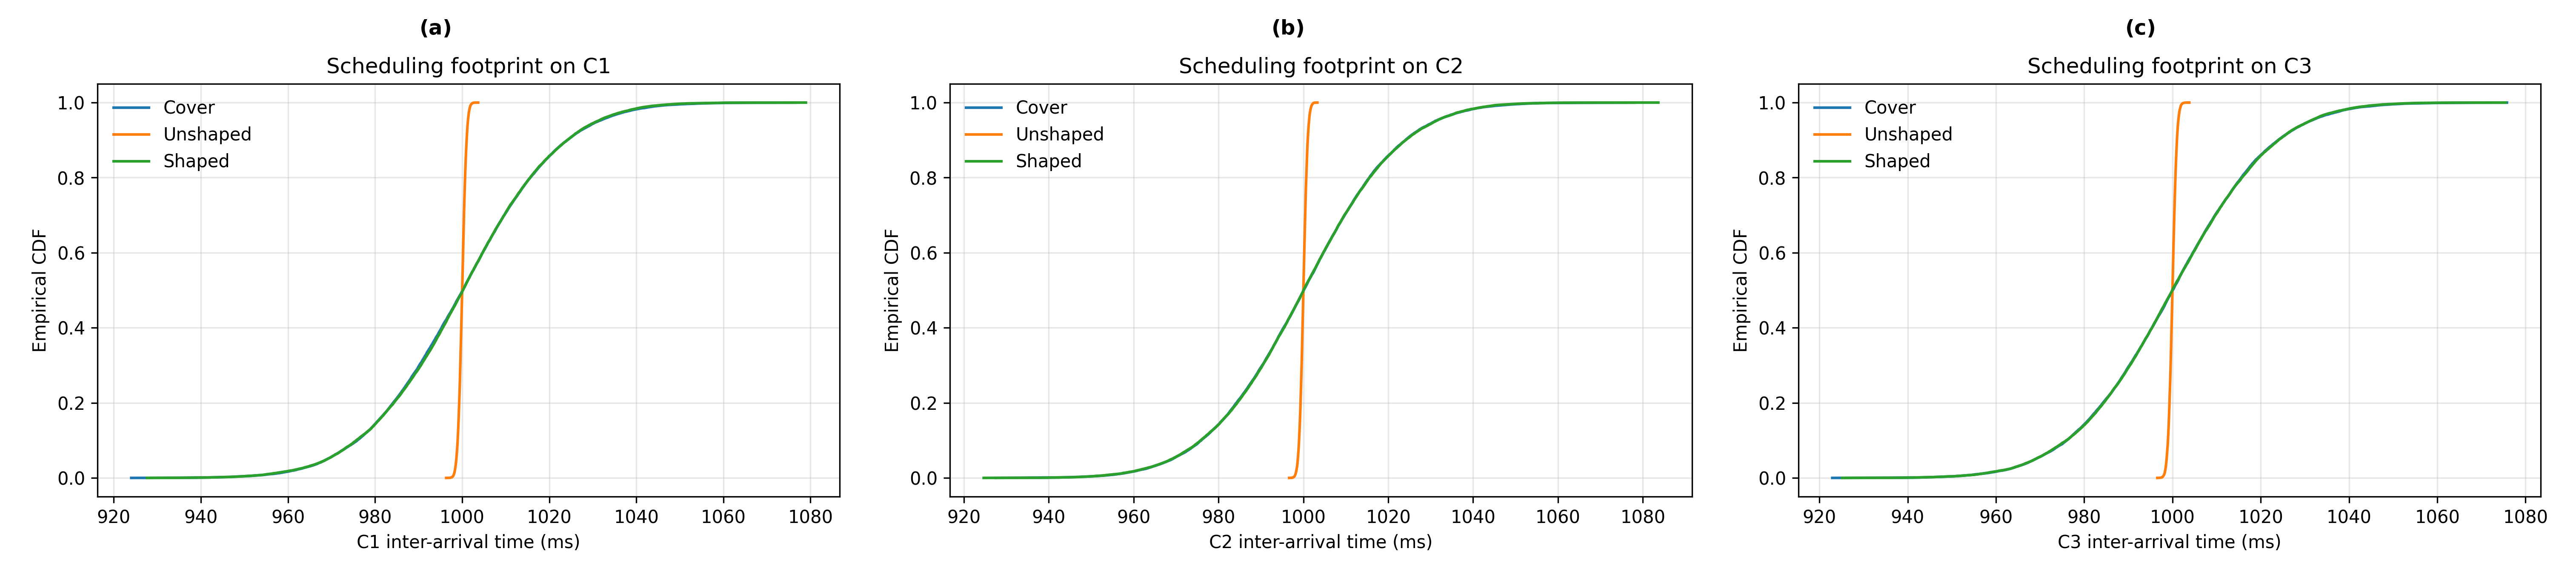
\includegraphics[width=\textwidth]
    {Figure_S1.png}
    \caption{Empirical cumulative distribution functions of the
    per-channel inter-arrival times for (a) $C_1$, (b) $C_2$, and
    (c) $C_3$ under the benign-cover, unshaped-protocol, and
    admissibly shaped schedules. The unshaped traces are concentrated
    within a narrow interval around the nominal $1000$-ms epoch
    period, producing a pronounced and consistent timing signature
    across the three channels. In contrast, the shaped distributions
    closely follow the corresponding cover distributions throughout
    their ranges. The overlap provides visual evidence that the
    admissible scheduler $\sigma^\star$ suppresses the marginal
    scheduling footprint while retaining the channel-specific
    temporal variability of the cover process.}
    \label{supp-fig:scheduling_ecdf_channels}
\end{figure*}


\begin{figure}[!t]
    \centering
    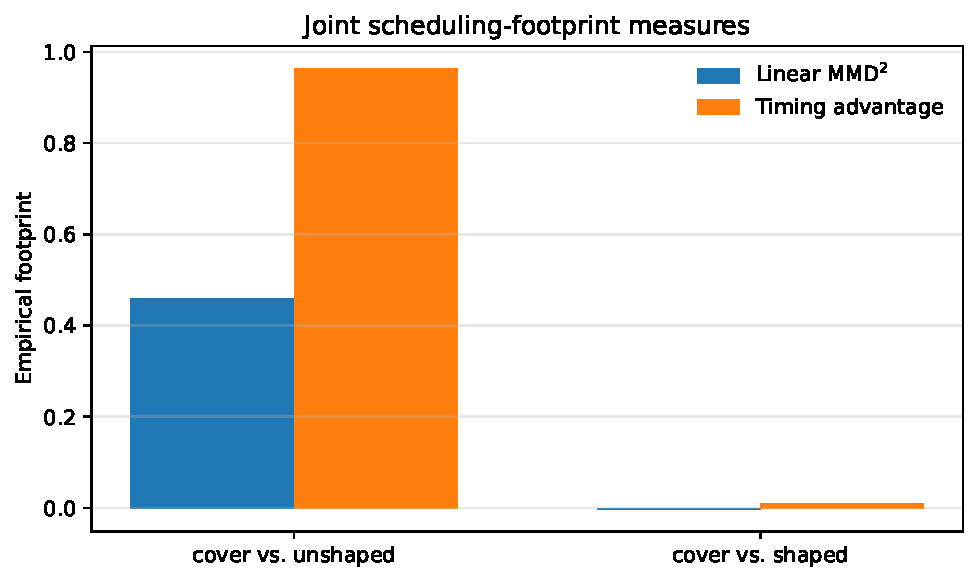
\includegraphics[width=\columnwidth]
    {Figure_S2.pdf}
    \caption{Joint multichannel scheduling-footprint measures for
    benign cover traffic compared with unshaped and admissibly shaped
    protocol traces. The linear-time RBF-kernel
    $\widehat{\operatorname{MMD}}_{\ell}^{\,2}$ measures the
    distributional difference in the joint epoch representation
    $\mathbf{x}_e=[X_{1,e},X_{2,e},X_{3,e},
    \operatorname{skew}_e,L_e]$, while the normalised timing advantage is $\widehat{\operatorname{Adv}}_{\mathsf{time}}^{\mathsf{norm}}
    =2|\widehat a-\tfrac{1}{2}|$.
    The large MMD estimate and near-unit timing advantage for the
    unshaped schedule indicate a readily identifiable multichannel
    timing signature. Following admissible shaping, the MMD permutation test
    does not reject the selected null and the timing
    advantage approaches zero, indicating chance-level discrimination
    between cover and shaped traces. The small negative shaped MMD
    estimate is a finite-sample property of the linear-time estimator;
    neither its sign nor non-rejection proves equal distributions.}
    \label{supp-fig:scheduling_joint}
\end{figure}


\begin{figure}[!t]
    \centering
    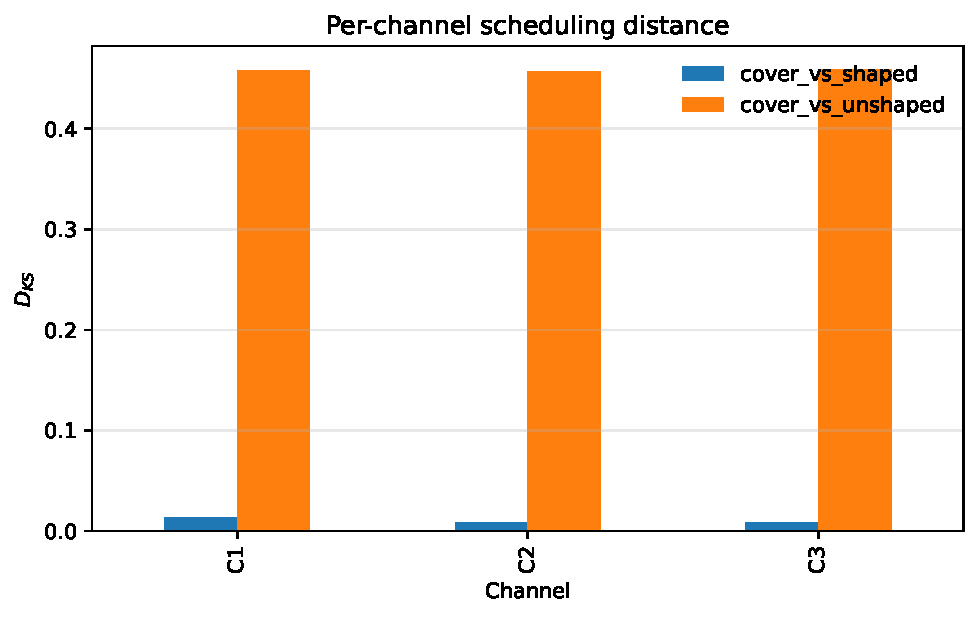
\includegraphics[width=\columnwidth]
    {Figure_S3.pdf}
    \caption{Per-channel scheduling footprint measured using the
    two-sample Kolmogorov--Smirnov distance $D_{\mathsf{KS}}$.
    The unshaped protocol traces exhibit large and consistent
    distributional differences from benign cover traffic across
    $C_1$, $C_2$, and $C_3$, with
    $D_{\mathsf{KS}}\approx0.46$. After applying the admissible
    scheduler $\sigma^\star$, the distances decrease to
    approximately $0.009$--$0.014$, showing that the shaped
    inter-arrival distributions closely reproduce the corresponding
    cover distributions. The consistently small shaped distances
    across all three channels provide empirical evidence that
    admissible shaping substantially suppresses the marginal timing
    footprint associated with
    $\varepsilon_{\mathsf{sched}}(\sigma^\star)$.}
    \label{supp-fig:scheduling_ks}
\end{figure}



\paragraph{Per-channel timing distributions.}
Table~\ref{tab:scheduling_ks} and
Fig.~\ref{supp-fig:scheduling_ks} show a clear separation between benign
cover traffic and the unshaped protocol. The unshaped comparison gives
$D_{\mathsf{KS}}=0.4582$, $0.4565$, and $0.4591$ on $C_1$, $C_2$,
and $C_3$, respectively, with $p<10^{-4}$ in every case. The
unshaped schedule is therefore strongly inconsistent with the benign
cover timing model. This result is also visible in the empirical
distribution functions: the unshaped trace is concentrated tightly
around the nominal $1000$-ms epoch period, producing an abrupt
near-step distribution, whereas the cover trace exhibits the wider
variation expected from the stochastic cover process.

Admissible shaping removes almost all of this per-channel discrepancy.
The shaped comparisons give
$D_{\mathsf{KS}}=0.0138$, $0.0088$, and $0.0085$ on $C_1$, $C_2$,
and $C_3$, respectively. Relative to the corresponding unshaped
values, these results represent reductions of approximately
$97.0\%$, $98.1\%$, and $98.1\%$, with an average reduction of
approximately $97.7\%$. The associated $p$-values are $0.2969$,
$0.8335$, and $0.8629$, so the null hypothesis of equal
per-channel distributions is not rejected under the selected test.
The selected KS test detected no per-channel difference in this
comparison. Non-rejection neither proves identical distributions nor
upper-bounds the remaining discrepancy.

The ECDFs in
Fig.~\ref{supp-fig:scheduling_ecdf_channels} support the same interpretation. On each channel, the shaped curve
closely follows the cover curve across the distribution, while the
unshaped curve remains narrowly concentrated around the nominal epoch
period. Consequently, the scheduler reproduces not only the cover
mean but also much of its temporal spread.

\begin{table*}[!t]
\centering
\caption[Per-channel scheduling-footprint comparison.]
{Per-channel scheduling-footprint comparison using the two-sample Kolmogorov--Smirnov test.}
\label{tab:scheduling_ks}
\small
\setlength{\tabcolsep}{6.0pt}
\renewcommand{\arraystretch}{1.15}
\begin{threeparttable}
\begin{tabular}{@{}llrrcc@{}}
\toprule
\textbf{Comparison} &
\textbf{Channel} &
\multicolumn{2}{c}{\textbf{Sample size}} &
\textbf{KS statistic} &
$\boldsymbol{p}$\textbf{-value} \\
\cmidrule(lr){3-4}
& & $\boldsymbol{n_0}$ & $\boldsymbol{n_1}$
& $\boldsymbol{D_{\mathrm{KS}}}$ \textbf{[95\% CI]} & \\
\midrule
\multirow{3}{*}{Cover vs. unshaped}
& $C_1$ & 10000 & 10000 & 0.4582 [0.4514, 0.4679] & $<10^{-4}$ \\
& $C_2$ & 10000 & 10000 & 0.4565 [0.4506, 0.4677] & $<10^{-4}$ \\
& $C_3$ & 10000 & 10000 & 0.4591 [0.4516, 0.4694] & $<10^{-4}$ \\
\addlinespace[2pt]
\multirow{3}{*}{Cover vs. shaped}
& $C_1$ & 10000 & 10000 & 0.0138 [0.0100, 0.0301] & 0.2969 \\
& $C_2$ & 10000 & 10000 & 0.0088 [0.0098, 0.0256] & 0.8335 \\
& $C_3$ & 10000 & 10000 & 0.0085 [0.0095, 0.0250] & 0.8629 \\
\bottomrule
\end{tabular}
\begin{tablenotes}
\footnotesize
\item \textit{Notes:} $n_0$ and $n_1$ are the numbers of cover and comparison traces, respectively. $D_{\mathrm{KS}}$ is the two-sample Kolmogorov--Smirnov statistic, and the bracketed values are 95\% bootstrap confidence intervals. The shaped samples have small observed marginal $D_{\mathrm{KS}}$ values and no rejection under this test. These findings do not establish distributional equality or a full-history scheduling bound.
\end{tablenotes}
\end{threeparttable}
\end{table*}

\paragraph{Joint multichannel footprint.}
The joint results in Table~\ref{tab:scheduling_joint} and
Fig.~\ref{supp-fig:scheduling_joint} confirm that the improvement is not
limited to independent channel marginals. For cover versus unshaped
traffic, the linear-time RBF estimate is
$\widehat{\operatorname{MMD}}_{\ell}^{\,2}=0.45879$, with
$p_{\mathsf{MMD}}=0.0010$. Thus, the combined vector of channel
inter-arrivals, cross-channel skew, and epoch latency remains strongly
distinguishable before shaping.

For cover versus shaped traffic, the estimate is
$\widehat{\operatorname{MMD}}_{\ell}^{\,2}=-0.00259$, with
$p_{\mathsf{MMD}}=0.6633$. The population quantity
$\operatorname{MMD}^{2}$ is non-negative; the small negative value is
a finite-sample outcome of the linear-time estimator and should be
reported with its non-rejecting permutation result, rather than
interpreted as a negative population distance or proof of equality. The permutation result therefore
provides no evidence of a joint distributional difference between the
cover and shaped traces under the selected feature representation.

The timing warden gives the same conclusion. It distinguishes cover
from unshaped traffic with accuracy $0.9821$ and
$\operatorname{AUC}=0.9930$, indicating that the unshaped schedule
contains an almost deterministic timing signature. For cover versus
shaped traffic, accuracy falls to $0.4947$ and
$\operatorname{AUC}=0.4919$, both close to random classification.
Moreover, the classifier-permutation test changes from
$p_{\mathsf{clf}}=0.0050$ for unshaped traffic to
$p_{\mathsf{clf}}=0.9154$ for shaped traffic.

The table reports the normalised timing advantage
\begin{equation}
\widehat{\operatorname{Adv}}_{\mathsf{time}}^{\mathsf{norm}}
=
2\left|
\widehat a-\frac{1}{2}
\right|,
\label{eq:supp_sched_norm_adv}
\end{equation}
which decreases from $0.9642$ to $0.0107$, a reduction of
approximately $98.9\%$. This normalised empirical diagnostic uses the
full acceptance-gap scale of the main formal games. The corresponding
half-scale guessing diagnostic is
\begin{equation}
\widehat{\operatorname{Adv}}_{\mathsf{time}}
=
\left|
\widehat a-\frac{1}{2}
\right|
=
\frac{1}{2}
\widehat{\operatorname{Adv}}_{\mathsf{time}}^{\mathsf{norm}},
\label{eq:supp_sched_half_adv}
\end{equation}
namely $0.4821$ for the unshaped trace and approximately $0.0054$
for the shaped trace. The half-scale values are reported only to make
the experimental conventions comparable. Neither scale converts this
fixed timing classifier into an upper bound on the formal scheduling loss;
see main Section~\ref{main-subsec:empirical-security-bridge}.

\begin{table*}[!t]
\centering
\caption[Joint multichannel scheduling-footprint results.]
{Joint multichannel scheduling-footprint results under distributional and classifier-based tests.}
\label{tab:scheduling_joint}
\small
\setlength{\tabcolsep}{5.0pt}
\renewcommand{\arraystretch}{1.15}
\begin{threeparttable}
\begin{tabular}{@{}lrrrrrr@{}}
\toprule
\textbf{Comparison} &
\multicolumn{2}{c}{\textbf{Distributional test}} &
\multicolumn{4}{c}{\textbf{Timing warden}} \\
\cmidrule(lr){2-3}
\cmidrule(l){4-7}
& $\boldsymbol{\mathrm{MMD}^{2}_{\ell}}$
& $\boldsymbol{p_{\mathrm{MMD}}}$
& \textbf{Accuracy}
& \textbf{AUC}
& $\boldsymbol{\widehat{\mathrm{Adv}}_{\mathsf{time}}^{\mathsf{norm}}}$
& $\boldsymbol{p_{\mathrm{clf}}}$ \\
\midrule
Cover vs. unshaped &  0.45879 & 0.0010 & 0.9821 & 0.9930 & 0.9642 & 0.0050 \\
Cover vs. shaped   & -0.00259 & 0.6633 & 0.4947 & 0.4919 & 0.0107 & 0.9154 \\
\bottomrule
\end{tabular}
\begin{tablenotes}
\footnotesize
\item \textit{Notes:} $\mathrm{MMD}^{2}_{\ell}$ is the linear-time, RBF-kernel estimate of the squared maximum mean discrepancy, with $p_{\mathrm{MMD}}$ obtained by permutation testing. The timing warden is evaluated using leave-one-seed-out classification. Its empirical advantage is $\widehat{\mathrm{Adv}}_{\mathsf{time}}^{\mathsf{norm}}=|2\,\mathrm{Accuracy}-1|$, and $p_{\mathrm{clf}}$ denotes the classifier significance test. A small negative $\mathrm{MMD}^{2}_{\ell}$ value can occur for an unbiased finite-sample estimator and should be interpreted as no detectable positive discrepancy.
\end{tablenotes}
\end{threeparttable}
\end{table*}

\paragraph{Operational cost and admissibility.}
Table~\ref{tab:scheduling_cost} shows that the shaped traffic closely
matches the operational profile of the cover process. Mean epoch
latency is $76.47$~ms for shaped traffic and $76.42$~ms for cover
traffic, a difference of only $0.05$~ms. The shaped P95 latency is
$117.50$~ms, compared with $117.84$~ms for cover traffic, while the
P95 cross-channel skew values are $16.35$ and $16.39$~ms,
respectively. Mean scheduling delay differs by only $0.06$~ms, and
the mean per-run emission rate remains approximately $1.000$ epoch/s
in both conditions. These
measurements show that shaping reproduces the cover timing profile
without reducing the simulated emission rate. Each of three seeds
contains 10,000 epochs at a nominal 1,000-ms period. Rates are computed
within each seed as epoch count divided by its send-time span and then
averaged; pooling seed counts over one overlapping time span would
spuriously triple the rate. This is an emission rate, not measured
authenticated receiver throughput.

The reduction in the tested timing footprint comes at a latency cost
relative to the unshaped schedule. Shaping increases mean latency from $30.94$ to
$76.47$~ms and P95 latency from $37.46$ to $117.50$~ms. It also
raises P95 skew from $3.94$ to $16.35$~ms. This is the expected
price of replacing an easily detectable near-periodic schedule with
cover-like temporal variation. Importantly, no admissibility violation
is observed in any tested condition. For the selected scheduler budget
$\rho$ and skew tolerance $\Delta$, the empirical rates satisfy
\begin{equation}
\widehat{\Pr}[D_e>\rho]=0,
\qquad
\widehat{\Pr}
\!\left[
\operatorname{skew}_e>\Delta
\right]
=0,
\label{eq:supp_sched_admissibility}
\end{equation}
over the evaluated traces. These are observed finite-sample rates and
should not be interpreted as a proof that the corresponding population
probabilities are exactly zero.


\begin{table*}[!t]
\centering
\caption[Operational cost and scheduler admissibility.]
{Operational cost and admissibility of the evaluated scheduling conditions.}
\label{tab:scheduling_cost}
\small
\setlength{\tabcolsep}{5.0pt}
\renewcommand{\arraystretch}{1.15}
\begin{threeparttable}
\begin{tabular}{@{}lrrrrrr@{}}
\toprule
\textbf{Condition} &
\multicolumn{2}{c}{\textbf{End-to-end latency}} &
\textbf{P95 skew} &
\textbf{Shaping delay} &
\textbf{Emission rate} &
\textbf{Violations} \\
\cmidrule(lr){2-3}
& \textbf{Mean (ms)}
& \textbf{P95 (ms)}
& \textbf{(ms)}
& \textbf{Mean (ms)}
& \textbf{(epochs/s)}
& \textbf{(\%)} \\
\midrule
Cover    & 76.42 & 117.84 & 16.39 & 50.46 & 1.000 & 0.0000 \\
Shaped   & 76.47 & 117.50 & 16.35 & 50.52 & 1.000 & 0.0000 \\
Unshaped & 30.94 &  37.46 &  3.94 &  6.50 & 1.000 & 0.0000 \\
\bottomrule
\end{tabular}
\begin{tablenotes}
\footnotesize
\item \textit{Notes:} P95 denotes the 95th percentile. P95 skew is the 95th-percentile inter-channel timing skew, while shaping delay is the additional delay introduced by the scheduling policy. Emission rate is averaged over the three seed-specific epoch-count/send-span
ratios; it excludes receiver computation. Violations report the proportion of
epochs exceeding the declared operational constraints.
\end{tablenotes}
\end{threeparttable}
\end{table*}

\paragraph{Connection to the security model.}
In the \emph{Formal Framework and Security Definition} of the main manuscript (see Section~\ref{main-subsec:formal}), $\Sigma$ denotes the class of admissible schedulers and
$\operatorname{Sched}(\cdot;\sigma)$ maps per-channel objects to timed
traces. The \emph{Multichannel Synchronization and
Re-synchronization} algorithm then uses an instantiated
$\sigma^\star\in\Sigma$ together with the sliding window $W$, timeout
$\tau$, skew tolerance $\Delta$, and heartbeat cadence $h$. In the
hybrid-composition theorem, the warden's advantage contains the
additive term
\begin{equation}
\mathsf{Adv}^{\mathsf{mc}}\le\varepsilon_{\mathsf{other}}
 +\varepsilon_{\mathsf{sched}}(\sigma^\star),
\label{eq:supp_sched_theory_link}
\end{equation}
where $\varepsilon_{\mathsf{other}}=\varepsilon_{\mathsf{KDF}}+
\varepsilon_{\mathsf{param}}+\varepsilon_{\mathsf{unl}}+
\mathsf{Adv}^{\mathsf{PRF}}_{\mathsf{synth}}+\varepsilon_{\mathsf{samp}}+
\varepsilon_{\mathsf{emb}}$ retains all preceding losses.
The scheduling term captures the full-view transition introduced by admissible transport shaping.

The finite synthetic experiment exhibits reduced selected timing
statistics after shaping:
\begin{align}
D_{\mathsf{KS}}
\!\left(
\mathcal T_{\mathsf{cover}},
\mathcal T_{\mathsf{shaped}}
\right)
&\ll
D_{\mathsf{KS}}
\!\left(
\mathcal T_{\mathsf{cover}},
\mathcal T_{\mathsf{unshaped}}
\right),\\
\widehat{\operatorname{MMD}}_{\ell}^{\,2}
\!\left(
\mathcal T_{\mathsf{cover}},
\mathcal T_{\mathsf{shaped}}
\right)
&\approx 0
\ll
0.45879,\\
\widehat{\operatorname{Adv}}_{\mathsf{time}}^{\mathsf{norm}}
\!\left(
\mathcal T_{\mathsf{cover}},
\mathcal T_{\mathsf{shaped}}
\right)
&=
0.0107
\ll
0.9642.
\end{align}
At the same time, Eq.~\eqref{eq:supp_sched_admissibility} shows that
the observed traces remain within the configured delay and skew
budgets. The experiment therefore provides empirical support for the
claim that the selected $\sigma^\star$ reduces an otherwise visible
timing signature while satisfying the operational constraints required
by the synchronisation algorithm.

These measurements should be interpreted as empirical proxies
associated with
$\varepsilon_{\mathsf{sched}}(\sigma^\star)$, rather than as a direct
estimate or upper bound on the corresponding joint computational transition loss.
The KS statistic examines one-dimensional channel marginals, MMD
examines the selected joint feature representation, and the classifier
measures distinguishability only within its hypothesis class.
Nevertheless, their agreement provides substantially stronger evidence
than any individual measure alone.

Finally, this experiment complements
Section~\ref{main-subsec:multichannel_robustness} of the main manuscript. That subsection distinguishes synthetic transport acceptance from
the real-image authentication and reconstruction checks. The
present experiment probes a synthetic scheduler and does not establish
authenticated image delivery under real network impairments. Together, the two evaluations
address both the operational and security roles of the scheduler.

\paragraph{Scope and limitation.}
The cover process in this experiment is a controlled stochastic timing
model. The results characterise the measured timing footprint under that
model and the selected warden; they do not establish indistinguishability
for every real-world traffic source. A deployment-level extension should repeat the same
KS, MMD, and timing-classification analysis using timestamps collected
from genuine benign application traffic.


\subsection{Communication Overhead and Runtime Efficiency}
\label{subsec:runtime_overhead}

This subsection reports fused-v3.2 image-component runtime and an
analytical binary-layout byte budget. The runtime summary covers 10,000
images per principal payload; it does not time the complete authenticated
receiver. The byte budget combines saved carrier sizes with assumed
control and heartbeat fields. It is not a measurement of the
\texttt{cpm-epoch-v2} JSON/base64 wire. Measured complete-protocol costs
appear in main Table~\ref{main-tab:revised-pilot} and
Appendices~\ref{sec:native-comparisons} and \ref{sec:hsmnet-comparison}.

\paragraph{Runtime efficiency.}
Table~\ref{tab:qim_v32_runtime} reports the mean embedding and extraction times, together with the resident-set-size (RSS) measurements. The embedding time remains practically stable over the evaluated payload range: it increases from $2.788\pm0.034$~s at $0.10$~bpp to $2.801\pm0.027$~s at $0.40$~bpp, corresponding to a relative increase of only approximately $0.47\%$. This weak dependence on the payload indicates that the dominant implementation cost arises from the fixed image-level operations used to construct and refine the
distortion map, including fused S-UNIWARD/MiPOD cost computation, complex feature analysis, region constraints, and STC processing, rather than from the number of embedded message bits alone.

Extraction is considerably faster than embedding. The mean
extraction time increases from $0.0813\pm0.0036$~s at
$0.10$~bpp to $0.0864\pm0.0041$~s at $0.40$~bpp, a relative
increase of approximately $6.27\%$. Across the three payloads,
extraction is approximately $32$--$34$ times faster than
embedding. The component timings describe only $T_{\mathsf{enc}}$ and
$T_{\mathsf{dec}}$. The complete protocol additionally incurs parameter
sampling, sender preflight, full-transcript authentication, masking and
protected state commitment. Its per-epoch costs are
\begin{align}
T_{\mathrm{epoch}}^{(\mathrm{snd})}
  &=
  O\!\left(
  T_{\mathrm{synth}}+T_{\mathrm{enc}}+T_{\mathrm{dec}}^{\mathrm{pre}}
  +T_{\mathrm{mac}}+T_{\mathrm{dither}}
  \right),\\
T_{\mathrm{epoch}}^{(\mathrm{rev})}
  &=
  O\!\left(
  T_{\mathrm{dec}}+T_{\mathrm{mac}}+T_{\mathrm{dither}}
  +T_{\mathrm{state}}
  \right),
\end{align}
because the sender performs the more expensive adaptive-cost
construction and embedding operation, whereas the receiver
primarily extracts the embedded bitstream and reconstructs the
mask. The measurements therefore provide empirical support for
the dominant $T_{\mathrm{enc}}$ and $T_{\mathrm{dec}}$ terms in
the complexity analysis. They do not measure full-protocol runtime or isolate the additional
terms in these expressions.

\begin{table*}[!t]
\centering
\caption[Runtime and memory use across payloads.]
{Runtime and memory use of QIM-Fused-CF across payloads.}
\label{tab:qim_v32_runtime}
\small
\setlength{\tabcolsep}{6pt}
\renewcommand{\arraystretch}{1.15}
\begin{threeparttable}
\begin{tabular}{@{}cccrrr@{}}
\toprule
\multicolumn{2}{c}{\textbf{Workload}} &
\multicolumn{2}{c}{\textbf{Runtime}} &
\multicolumn{2}{c}{\textbf{Memory}} \\
\cmidrule(lr){1-2}
\cmidrule(lr){3-4}
\cmidrule(l){5-6}
\textbf{Payload} &
\textbf{Images} &
\boldmath$T_{\mathsf{enc}}$ &
\boldmath$T_{\mathsf{dec}}$ &
\textbf{Mean RSS} &
\textbf{Peak RSS} \\
\textbf{(bpp)} &
{} &
\textbf{(s)} &
\textbf{(s)} &
\textbf{(MB)} &
\textbf{(MB)} \\
\midrule
0.10 & 10,000 & $2.788 \pm 0.034$ & $0.0813 \pm 0.0036$ & $643.6 \pm 25.4$ & $677.3 \pm 28.0$ \\
0.20 & 10,000 & $2.790 \pm 0.028$ & $0.0829 \pm 0.0034$ & $727.8 \pm 23.9$ & $762.1 \pm 26.1$ \\
0.40 & 10,000 & $2.801 \pm 0.027$ & $0.0864 \pm 0.0041$ & $808.4 \pm 24.2$ & $842.5 \pm 27.3$ \\
\bottomrule
\end{tabular}
\begin{tablenotes}
\footnotesize
\item \textit{Notes:} Embedding and memory summaries cover all 10,000 attempts per payload.
Extraction-time summaries have 9,999/9,996/9,996 finite observations at
0.10/0.20/0.40 bpp; unavailable extraction times are omitted. Values are
mean~$\pm$~sample standard deviation from the 153-column fused-v3.2
log partition; the appended 178-column 0.30-bpp block is excluded.
$T_{\mathsf{enc}}$ and $T_{\mathsf{dec}}$ are component times, not full
endpoint times. RSS denotes resident-set size. No GPU memory was allocated.
\end{tablenotes}
\end{threeparttable}
\end{table*}

\paragraph{Memory consumption.}
Memory use is more sensitive to the payload than execution time.
Mean RSS increases from $643.6\pm25.4$~MB at $0.10$~bpp to
$808.4\pm24.2$~MB at $0.40$~bpp, an increase of approximately
$25.6\%$. Peak RSS similarly rises from
$677.3\pm28.0$~MB to $842.5\pm27.3$~MB, corresponding to an
increase of approximately $24.4\%$. This behaviour is consistent
with the larger message, coding, and intermediate cost structures
required at higher payloads. GPU allocation and reservation are
zero for all payloads, confirming that the reported implementation
executed on the CPU.

These process-level RSS values should be distinguished from the
protocol-level receiver-buffer bound. The formal memory analysis
models the receiver state as
\begin{equation}
\operatorname{Space}
=O(WcL_{\max})+O\!\left(B_{\mathsf{acc}}(|H|+3|n|)\right),
\end{equation}
where $W$ is the sliding-window size, $c=3$ is the channel count,
$L_{\max}$ bounds retained frame bytes and $B_{\mathsf{acc}}$ counts
persisted accepted epochs. The RSS measurements additionally include the complete
embedding implementation, image arrays, cost maps, segmentation
structures, and Python runtime. They therefore characterise
practical implementation memory rather than directly estimating
the receiver's bounded re-synchronisation buffer.

\paragraph{Communication overhead.}
For a $512\times512$ grayscale carrier and payload $p$~bpp, the
nominal secret size is
\begin{equation}
B_m(p)
=
\left\lceil
\frac{p(512)(512)}{8}
\right\rceil
\quad\text{bytes}.
\end{equation}
This gives $3{,}277$, $6{,}554$, and $13{,}108$ bytes at
$0.10$, $0.20$, and $0.40$~bpp, respectively. The total
communication cost of one protocol epoch is represented as
\begin{equation}
B_{\mathrm{epoch}}
=
B_s
+
B_{\gamma_1}
+
B_{\gamma_2}
+
B_{\mathrm{ctrl}}
+
B_{\mathrm{hb}},
\end{equation}
where $B_s$ is the serialised stego-object size,
$B_{\gamma_1}+B_{\gamma_2}$ is the combined size of the two
cover messages, $B_{\mathrm{ctrl}}$ contains the three epoch
headers, three nonces, framing fields, and MAC, and
$B_{\mathrm{hb}}$ is the amortised heartbeat cost.

As shown in Table~\ref{tab:qim_v32_overhead}, the assumed binary
layout assigns a fixed control cost of $218$ bytes per epoch,
while heartbeats add an amortised $12$ bytes. Hence, the combined
control and heartbeat cost is only $230$ bytes, or approximately
$0.088\%$ of the mean $262{,}519.2$ bytes transmitted per epoch.
The two cover messages contribute approximately $130.2$ bytes
($0.050\%$), whereas the $262{,}159$-byte stego-object accounts
for approximately $99.863\%$ of the transmitted data. The
communication cost is therefore dominated by the fixed-size
uncompressed image representation rather than by protocol
headers, nonces, MACs, or cover text.

\begin{table*}[!t]
\centering
\caption[Per-epoch communication accounting across payloads.]
{Analytical binary-layout communication budget using saved image sizes.}
\label{tab:qim_v32_overhead}
\small
\setlength{\tabcolsep}{4.4pt}
\renewcommand{\arraystretch}{1.15}
\begin{threeparttable}
\begin{tabular}{@{}ccrrrrrrr@{}}
\toprule
\multicolumn{2}{c}{\textbf{Payload setting}} &
\multicolumn{3}{c}{\textbf{Protocol data (B)}} &
\multicolumn{2}{c}{\textbf{Control traffic (B)}} &
\multicolumn{2}{c}{\textbf{Overall}} \\
\cmidrule(lr){1-2}
\cmidrule(lr){3-5}
\cmidrule(lr){6-7}
\cmidrule(l){8-9}
\textbf{Payload} &
\textbf{Saved files} &
\textbf{Secret} &
\textbf{Cover params.} &
\textbf{Stego-object} &
\textbf{Fixed} &
\textbf{Heartbeat} &
\textbf{Total (B)} &
\textbf{Expansion} \\
\textbf{(bpp)} &
{} &
{} &
{} &
{} &
{} &
{} &
{} &
{} \\
\midrule
0.10 & 9,999 &  3,277 & 130.2 & 262,159.0 & 218 & 12.0 & 262,519.2 & $80.11\times$ \\
0.20 & 9,996 &  6,554 & 130.2 & 262,159.0 & 218 & 12.0 & 262,519.2 & $40.05\times$ \\
0.40 & 9,996 & 13,108 & 130.2 & 262,159.0 & 218 & 12.0 & 262,519.2 & $20.03\times$ \\
\bottomrule
\end{tabular}
\begin{tablenotes}
\footnotesize
\item \textit{Notes:} Except for the saved-file count and expansion factor, entries are bytes per
hypothetical epoch under the stated binary layout, without JSON/base64 or
network headers. The saved-file counts are 9,999/9,996/9,996 and are
distinct from the 10,000-attempt runtime denominators. ``Cover params.'' denotes the combined transmitted size of the two cover-parameter sequences. Fixed control traffic comprises the constant-size epoch header, nonces, and authentication fields; heartbeat traffic is amortised per epoch. The stego-object is protocol data, not control overhead. Expansion is computed as total transmitted bytes divided by secret-message bytes.
\end{tablenotes}
\end{threeparttable}
\end{table*}
This analytical layout assigns fixed-size metadata a constant additive
cost independent of secret length $\ell$. Its 230-byte control/heartbeat
budget is an assumption of this layout, not an observed cost of the
complete-epoch wire.'' The stego-object is
not classified as control overhead because it is the carrier
transmitted on $C_3$.

Communication efficiency improves as more of the fixed-size
carrier capacity is used. Defining
\begin{equation}
\eta_{\mathrm{comm}}
=
\frac{B_m}{B_{\mathrm{epoch}}},
\qquad
R_{\mathrm{exp}}
=
\frac{B_{\mathrm{epoch}}}{B_m},
\end{equation}
the payload efficiency increases from approximately $1.25\%$ at
$0.10$~bpp to $4.99\%$ at $0.40$~bpp, while the corresponding
expansion ratio decreases from $80.11\times$ to $20.03\times$.
Thus, increasing the payload improves byte efficiency because the
same image carrier transports a larger secret. This benefit must
not be interpreted in isolation: the detectability experiments
show that larger payloads may expose stronger embedding traces.
The operational payload should therefore be selected by balancing
communication efficiency, memory use, and steganalytic security,
rather than by minimising the expansion ratio alone.

\paragraph{Overall assessment.}
The component runtime summary shows that adaptive embedding is more
expensive than extraction in this configuration. The analytical binary
layout assigns control fields a fixed small fraction of its byte budget;
that fraction does not describe the complete-epoch JSON/base64 wire.
The main practical trade-off is consequently not header overhead,
but the relationship among payload utilisation, memory
consumption, embedding time, and detectability.

%\paragraph{Hardware and software environment.}
%The measurements were obtained on [CPU model and core count] with [RAM] running [Ubuntu version], [Python version], and [storage type]. The implementation used CPU execution; no GPU memory was allocated.







% Appendices continue without resetting their letters.
\section{Detector-Wise and Epoch-Wise Steganalysis Behaviour}\label{Detector-Wise}

\begin{figure}
    \centering
    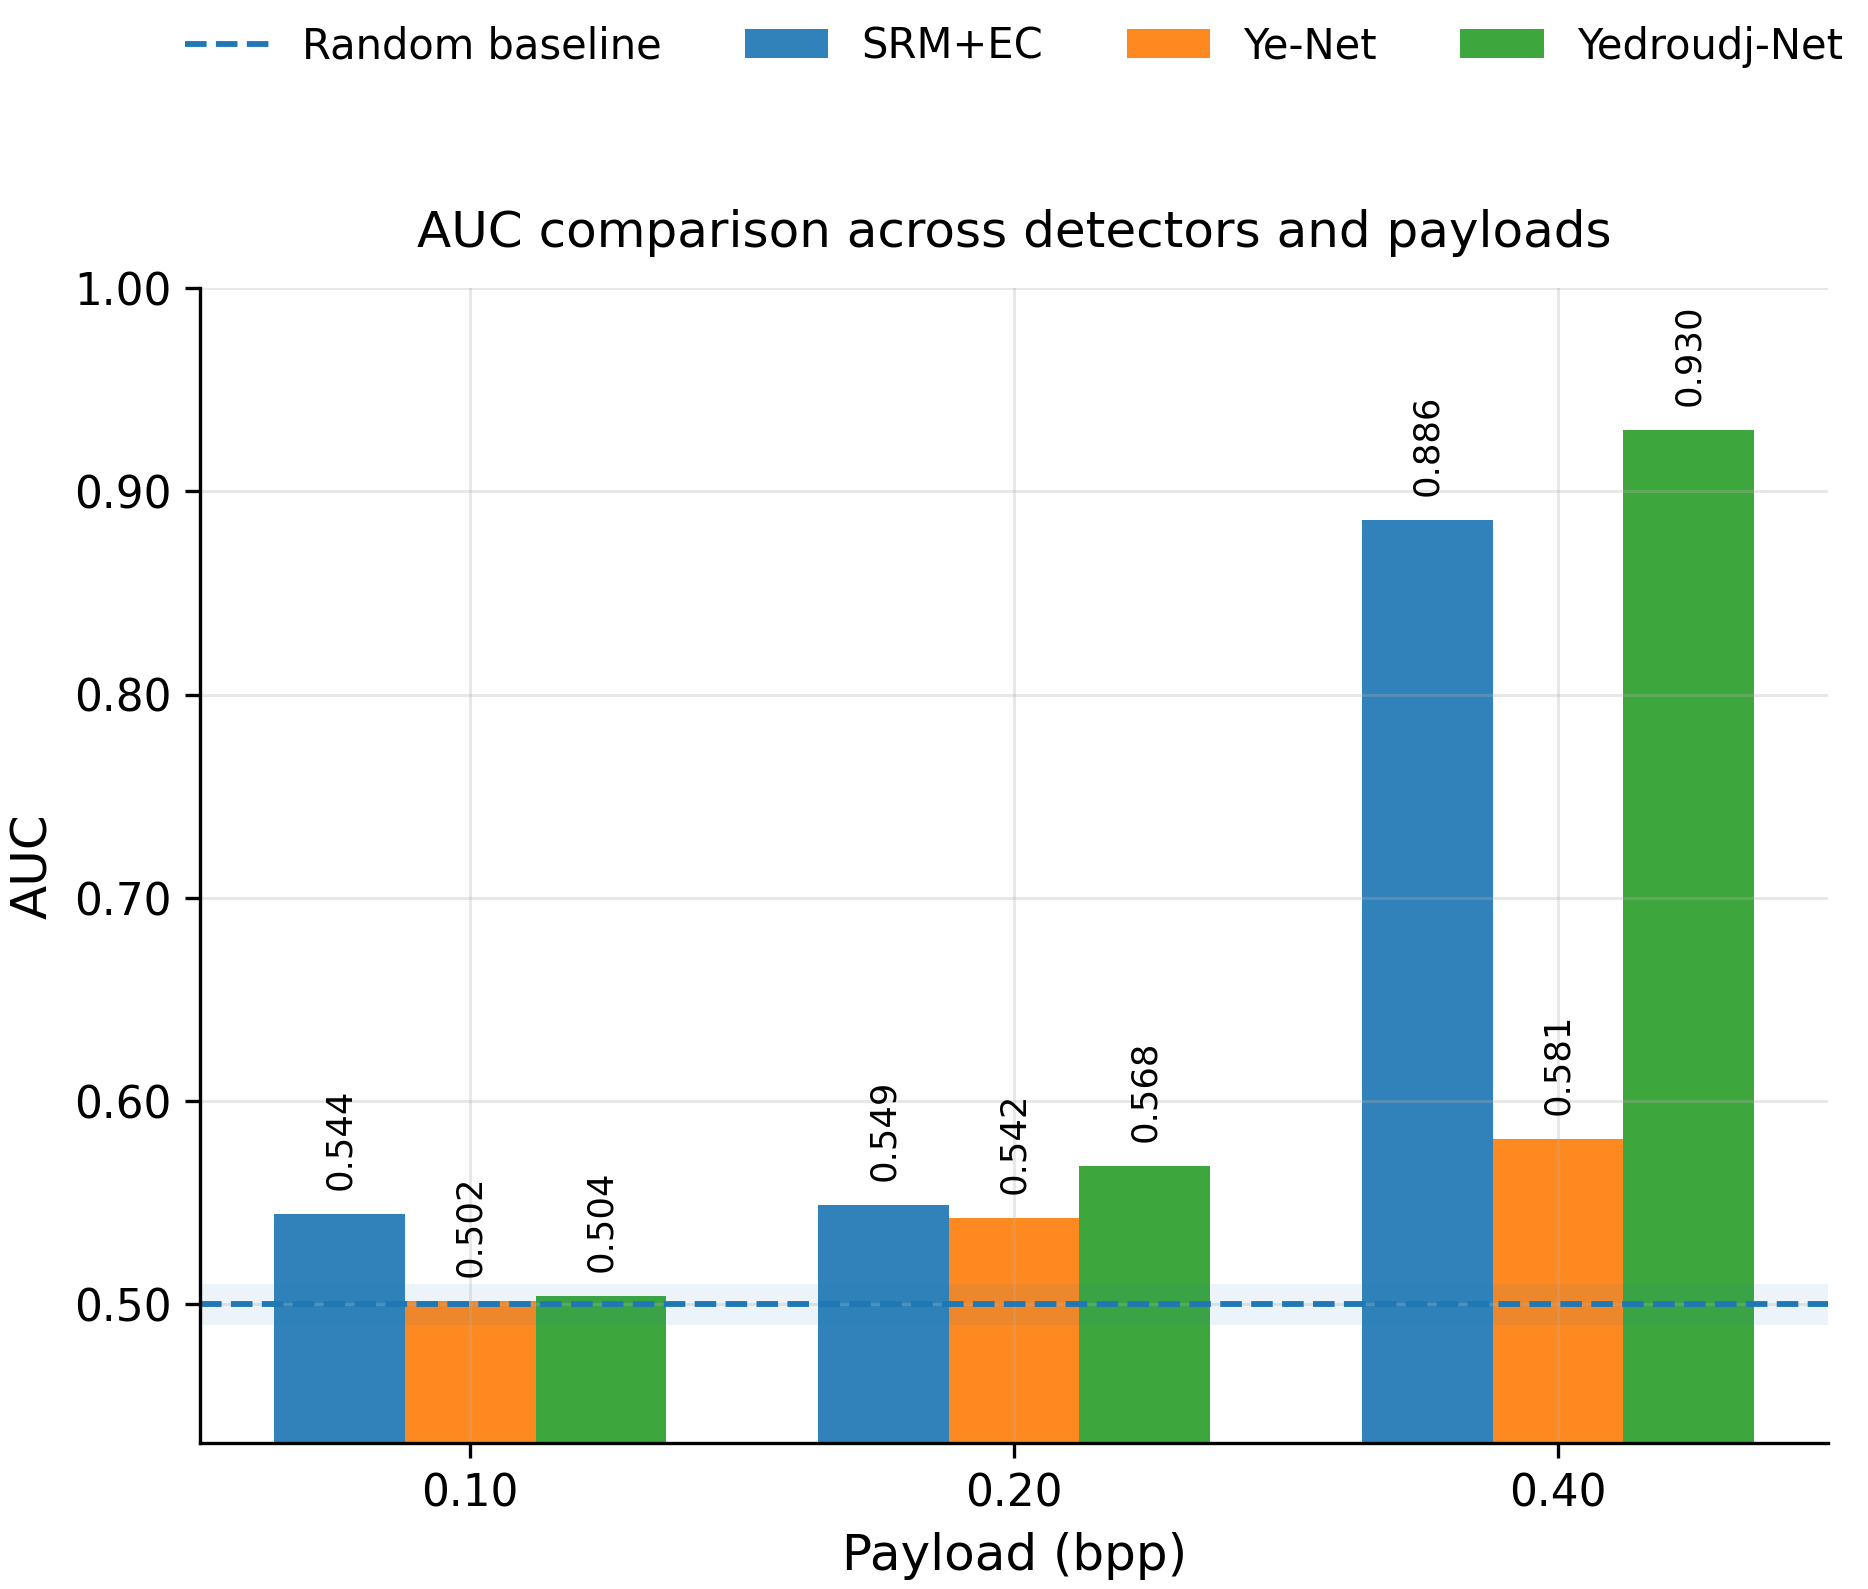
\includegraphics[width=0.9\linewidth]{Figure_S4.png}
    \caption{Test-set AUC of SRM+EC, Ye-Net, and Yedroudj-Net for QIM-Fused-CF at payloads of 0.10, 0.20, and
    0.40~bpp. The dashed horizontal line denotes random discrimination at $\mathrm{AUC}=0.5$. All detectors remain close to chance at 0.10~bpp and exhibit only limited discrimination at 0.20~bpp. At 0.40~bpp, SRM+EC and Yedroudj-Net achieve substantially stronger detection, whereas Ye-Net remains comparatively weak.}
    \label{Figure_S2}
\end{figure}


\begin{figure*}
    \centering
    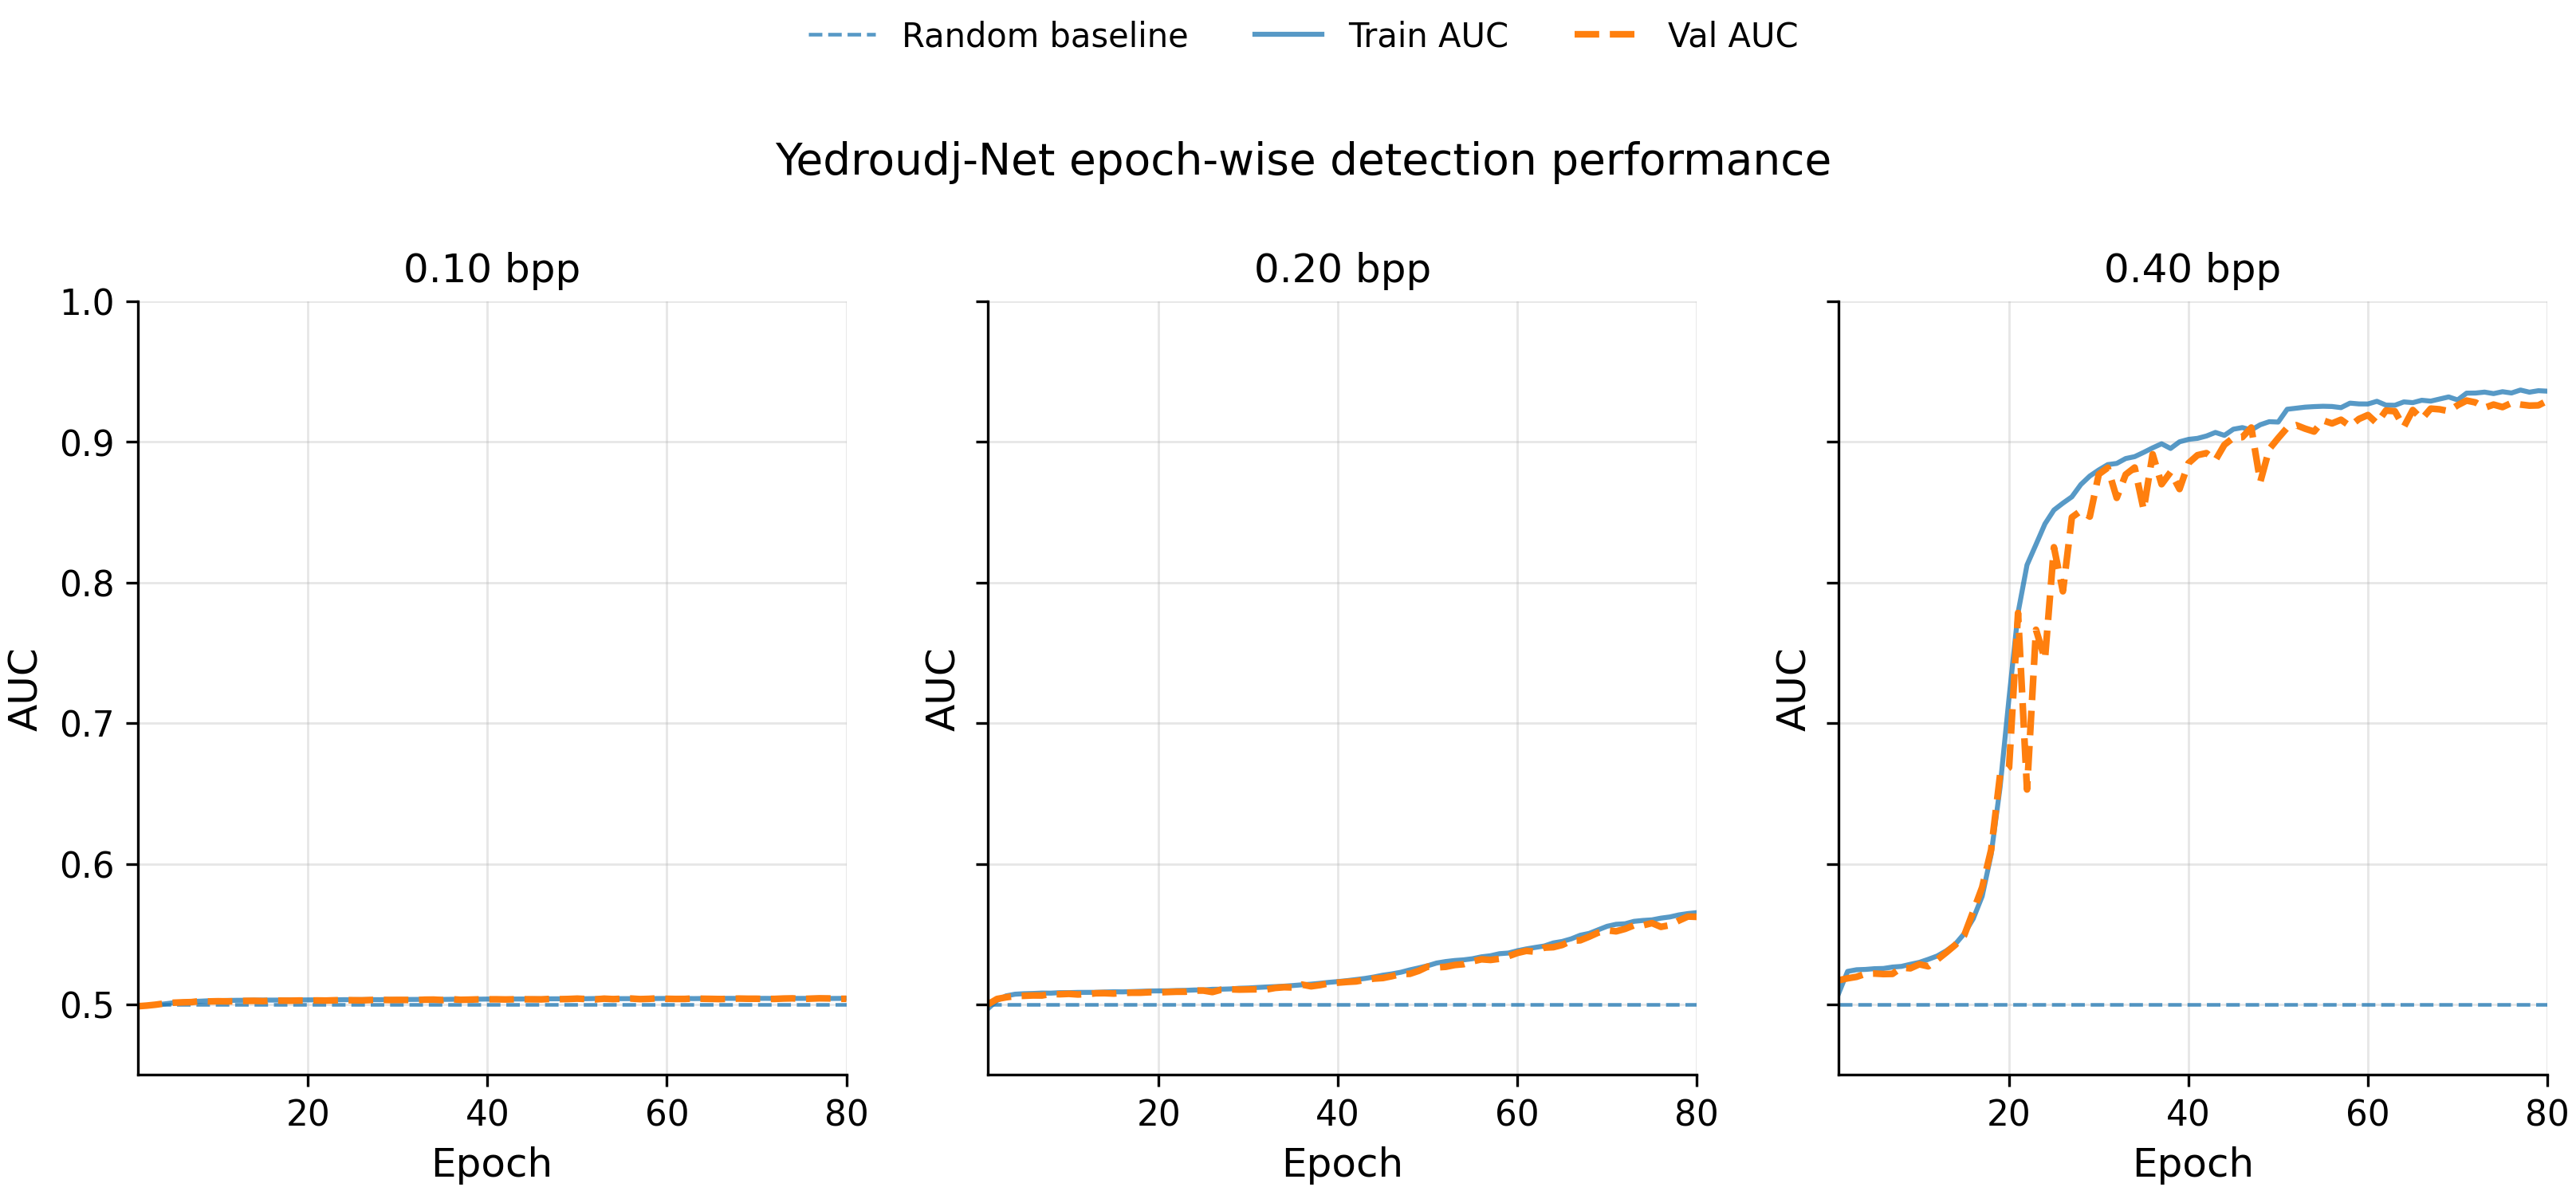
\includegraphics[width=0.9\textwidth]{Figure_S5.png}
    \caption{Training and validation AUC trajectories of Yedroudj-Net over 80 epochs at payloads of 0.10, 0.20, and 0.40~bpp. The dashed horizontal line marks random discrimination at $\mathrm{AUC}=0.5$. Performance remains near chance throughout training at 0.10~bpp, increases gradually at 0.20~bpp, and converges to a strong and stable detector at 0.40~bpp. The close agreement between the training and validation curves indicates limited generalisation disparity under the evaluated data split.}
    \label{Figure_S3}
\end{figure*}

\begin{figure*}[!t]
    \centering
    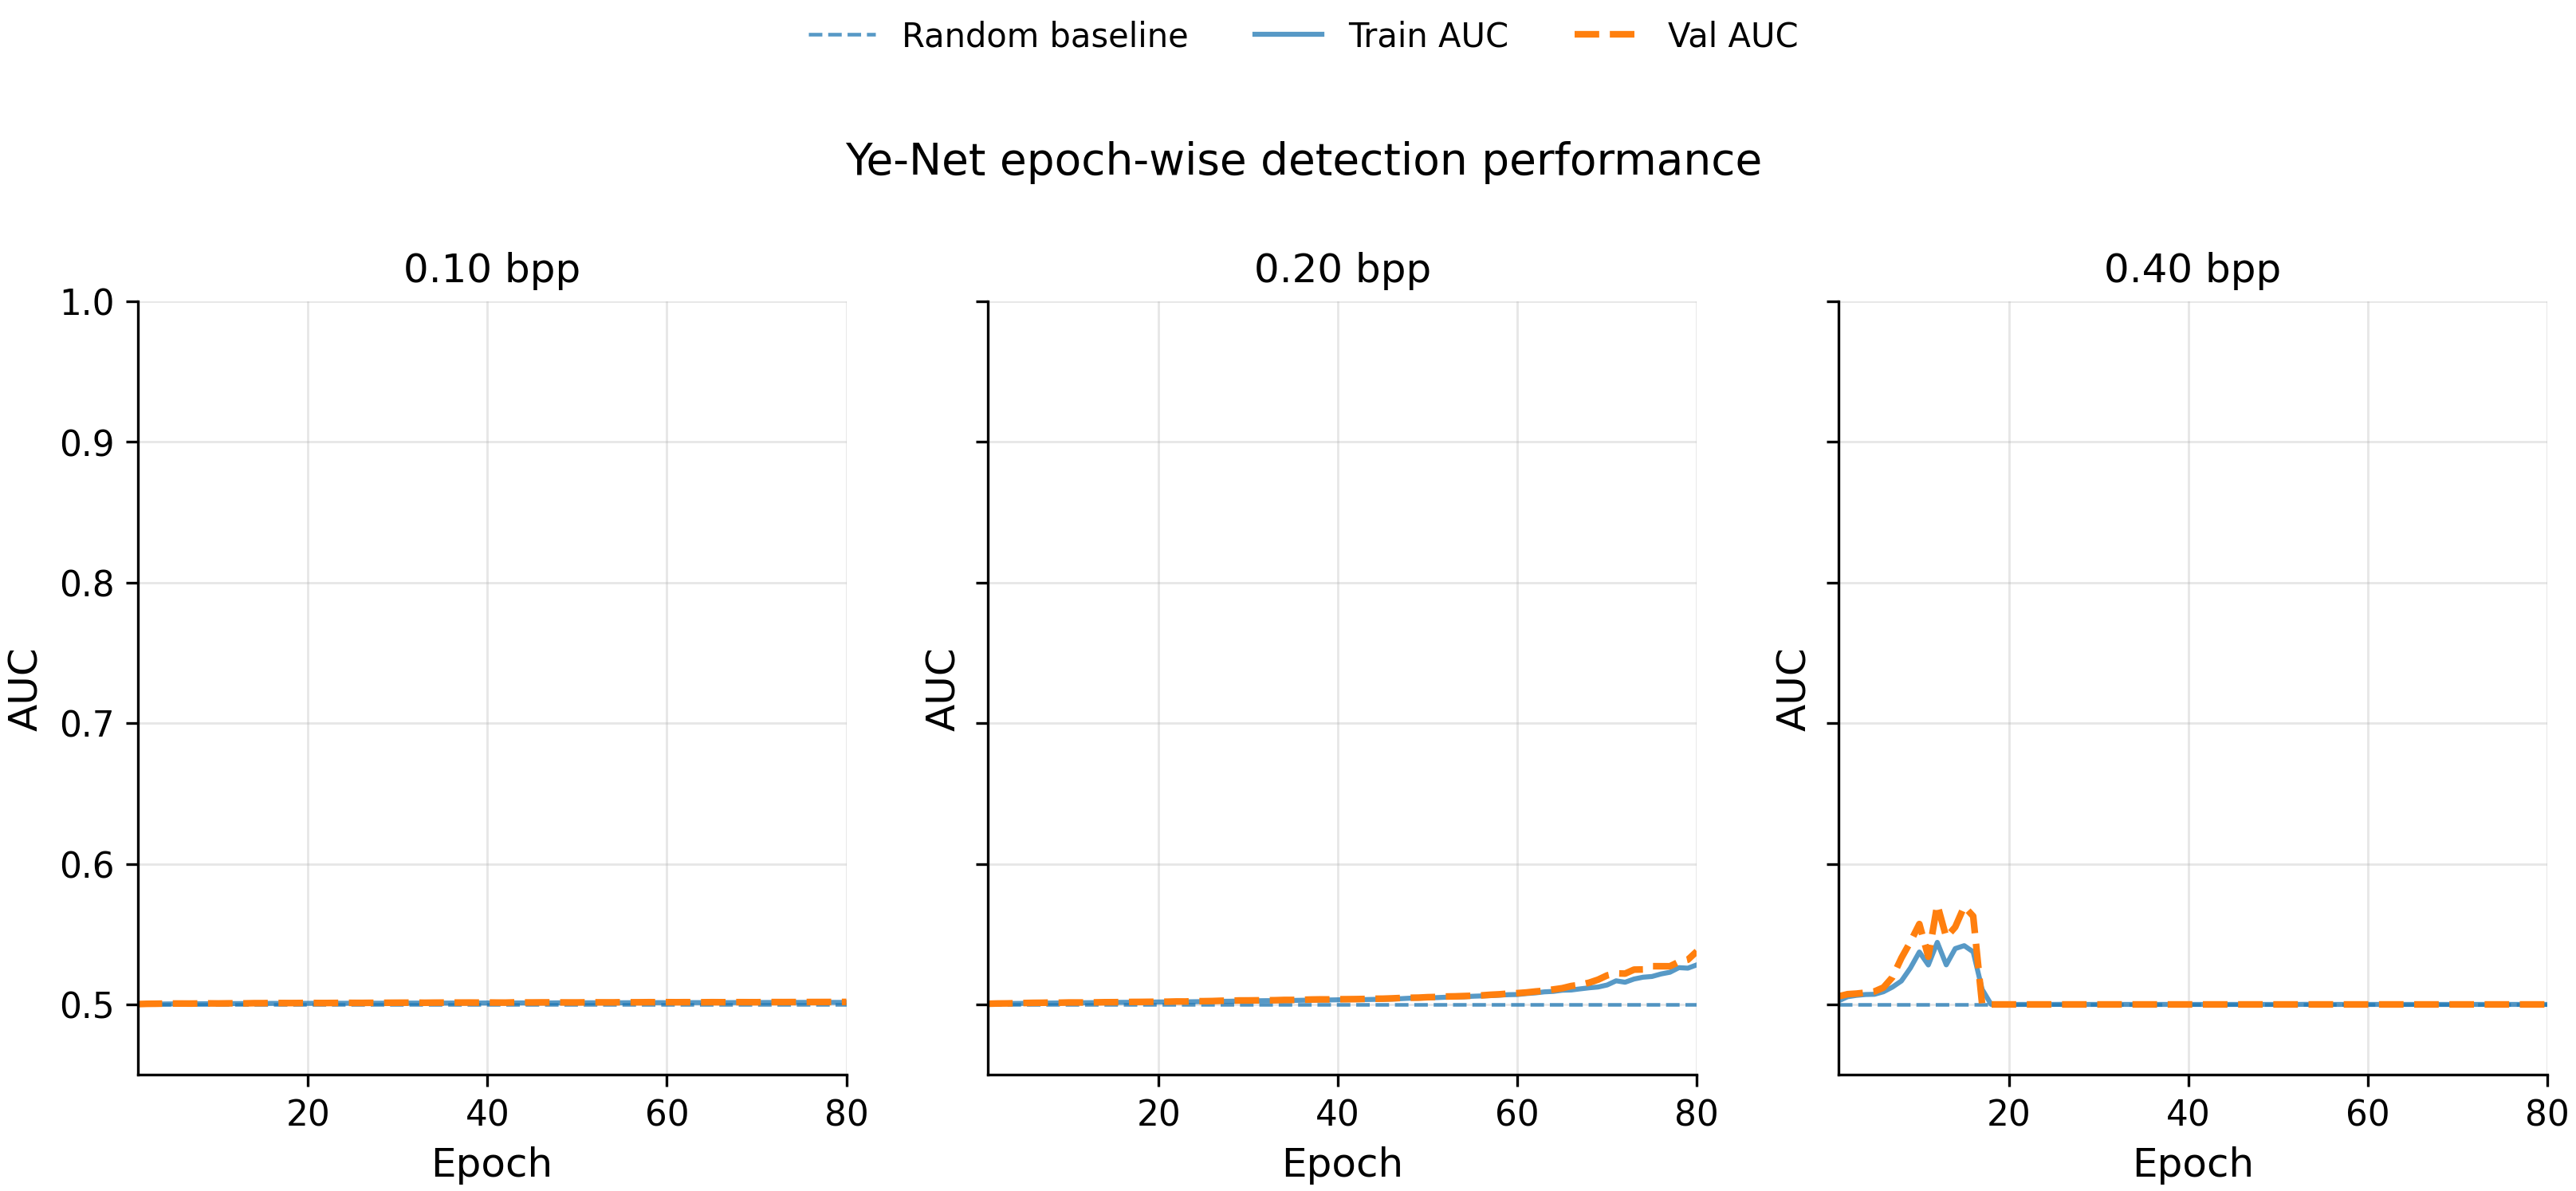
\includegraphics[width=\textwidth]{Figure_S6.png}
    \caption{Training and validation AUC trajectories of Ye-Net over 80 epochs at payloads of 0.10, 0.20, and 0.40~bpp. The dashed horizontal line denotes random discrimination at $\mathrm{AUC}=0.5$. The detector remains near chance at 0.10~bpp and improves only gradually at 0.20~bpp. At 0.40~bpp, the AUC initially increases before collapsing to chance-level performance after approximately epoch 17. The reported test result uses the checkpoint selected by validation AUC, as specified in Section~\ref{subsec:repro-cnn}.}
    \label{Figure_S4}
\end{figure*}

The principal test-set findings and their relationship to the
embedding term $\varepsilon_{\mathsf{emb}}$ are discussed in
Section~\ref{main-subsec:detectability_results} of the main
manuscript; the present supplement provides the corresponding
detector-wise AUC comparisons and complete 80-epoch learning
trajectories.

The detector comparison in Fig.~\ref{Figure_S2}
confirms that stego-object detectability increases with payload.
At 0.10~bpp, SRM+EC, Ye-Net, and Yedroudj-Net obtain AUC
values of 0.544, 0.502, and 0.504, respectively, indicating
near-random discrimination. Only limited improvement is observed
at 0.20~bpp, where Yedroudj-Net provides the strongest result
with an AUC of 0.568. At 0.40~bpp, however, SRM+EC and
Yedroudj-Net reach AUC values of 0.886 and 0.930, demonstrating
that the increased embedding footprint becomes detectable by both
hand-crafted residual features and learned CNN representations.
Ye-Net remains comparatively weak at this payload, with an AUC
of 0.581.

The complete 80-epoch trajectories in
Figs.~\ref{Figure_S3} and
\ref{Figure_S4} clarify the learning behaviour behind
these results. Yedroudj-Net remains near chance at 0.10~bpp,
learns a weak but consistent signal at 0.20~bpp, and converges
to approximately 0.93 AUC at 0.40~bpp with closely aligned
training and validation curves. Ye-Net similarly remains near
chance at 0.10~bpp and improves only gradually at 0.20~bpp.
At 0.40~bpp, it reaches an early validation maximum before
collapsing to chance-level performance, thereby justifying the use
of the epoch-12 checkpoint reported in the main results table.
The validation-selected checkpoint is reported according to the fixed
selection rule; a low final-epoch AUC is not evidence of carrier
undetectability.

The fixed-detector observations show weak measured discrimination at
$0.10$ bpp and strong detection by Yedroudj-Net and SRM+EC at $0.40$ bpp.
They do not upper-bound $\varepsilon_{\mathsf{emb}}$ against all wardens
or establish its value for the complete-epoch protocol. Ye-Net's weaker result
is not used to infer security at high payload.

\section{Applications}\label{sec:applications}
The following applications are illustrative model instantiations with
explicit mathematical interfaces. The reference experiments evaluate
only the PGM/STC carrier; they do not demonstrate banking, industrial or
ledger deployment. Each alternative carrier requires a specified blind
codec, admissible semantic domain and authenticated framing. The masking
and complete-epoch authentication rules remain those of the main protocol.

\subsection{Application to SMS-Centric Mobile Banking}
\label{Application in SMS Mobile Banking}

In constrained mobile-banking environments where SMS remains a
primary low-bandwidth interface
\cite{gomez2014simple,vishnuvardhan2020study,saxena2014easysms,
Joshi2019A,Giménez2019Extending,Castiglione2015Secure},
communication may traverse infrastructure that cannot be assumed
to provide end-to-end confidentiality or integrity
\cite{Salman2023SMS,Riaz2018Development,Ardagna2009Privacy,
Reddy2017An,Fathi2013SMS}. An active adversary may therefore
observe, delay, replay, or modify transmitted messages
\cite{barkancipher2003cryptanalysis,nohl2017ss7,
meyer2004guitar}.

The protocol of
Section~\ref{main-Hybrid_Entropy_Steganographic_Communication_Protocol}
can be instantiated by transmitting two message-independent,
benign cover-parameter objects
$\gamma_{1,e}$ and $\gamma_{2,e}$ over $C_1$ and $C_2$.
These objects may be generated from application-approved
non-transactional SMS templates or other semantically innocuous
mobile-banking content. They are converted to masking parameters
through
\begin{equation}
P_{\mathsf{params},e}
=
\mathsf{ParamExtract}
\left(
\gamma_{1,e},\gamma_{2,e}
\right),
\end{equation}
after which the transaction payload is protected as
\begin{equation}
b_e
=
F_{\mathsf{mask}}
\left(
m_e,P_{\mathsf{params},e};\eta_e
\right)
=
m_e\oplus\mu_e .
\label{eq:sms-masked-payload}
\end{equation}

The masked payload $b_e$, rather than the plaintext transaction
$m_e$, is embedded into an application-compatible object $s_e$
carried on $C_3$. Depending on the deployment, $C_3$ may be an
existing mobile-web, application, receipt, image, or other
low-bandwidth data channel. Thus, the complete protocol epoch is
distributed across several carriers and is not assumed to fit
within a single SMS message.

For SMS-based cover-parameter channels, synthesis must respect
the applicable encoding, segmentation, and semantic constraints.
An admissible cover object may therefore be required to satisfy
\begin{equation}
\gamma_{k,e}\in\mathcal{G}_{\mathsf{SMS}},
\qquad
\mathsf{Sem}(\gamma_{k,e})=\mathsf{benign},
\qquad
k\in\{1,2\},
\label{eq:sms-admissibility}
\end{equation}
where $\mathcal{G}_{\mathsf{SMS}}$ denotes the deployment's
permitted message class. In particular, auxiliary covers should
not themselves trigger financial actions or alter account state.

The three channel components are bound to the same authenticated
epoch. The receiver first performs header alignment, freshness
verification, and complete-transcript authentication according to
Algorithm~\ref{main-alg:mc-sync}. Only after these checks succeed
does it extract $\widehat b_e$, regenerate the same mask
$\mu_e$, and recover
\begin{equation}
\widehat m_e
=
\widehat b_e\oplus\mu_e .
\end{equation}
Stale, incomplete, malformed, or unauthenticated epochs are
rejected.

Security does not rely on any one channel remaining hidden from
the adversary. Under full cross-channel observation, concealment
is governed by the cover-parameter, embedding, unlinkability, and
scheduling terms of the \textsf{IND-STEGO-MC} analysis, while
message recovery is bounded separately by the keyed masking
analysis and active modification is handled by the replay and
authenticated-substitution results. See
Theorem~\ref{main-thm:composition},
Claim~\ref{main-Claim2}, and
Claims~\ref{main-Claim3}--\ref{main-Claim4}.

The construction is therefore a proposed mapping for
asynchronous, low-frequency banking instructions and
notifications for which several logically distinct communication
carriers are available. Its use for time-critical authentication
or transaction-authorisation workflows would require additional
deployment-specific latency, availability, and regulatory
analysis.

\subsection{IoT and Industrial Control Systems}
\label{app:iot}

Cyber-physical environments such as smart factories, industrial
control systems (ICS), and critical infrastructure operate under
strict timing, reliability, and safety constraints
\cite{nist80082r3}, while potentially being exposed to passive
surveillance and active network manipulation
\cite{cisa_aa24_249a2024,opswatsans2025}. A multivariate
telemetry stream observed over $T$ discrete time steps may be
written as
\begin{equation}
\label{eq:telemetry}
\mathbf{y}
=
\left(
y_1,\ldots,y_T
\right),
\qquad
y_t\in\mathbb{R}^{d},
\end{equation}
where $y_t(i)$ denotes the $i$th process or sensor variable at
time $t$.

Any steganographic modification must remain within an
application-defined admissible region. A simple abstraction is
\begin{equation}
\label{eq:iot-admissibility}
\|\mathbf{y}-\mathbf{y}'\|_{\infty}
\leq
\epsilon,
\qquad
|\Delta t|
\leq
\delta,
\end{equation}
where $\epsilon$ bounds permitted value perturbation and
$\delta$ bounds additional timing deviation. These constraints
must be selected so that the modified stream remains compatible
with the relevant physical, semantic, and control-system
requirements. For example, for a discrete-time linear closed loop,
a nominal stability requirement may be expressed as
\begin{equation}
\label{eq:iot-stability}
\rho(A-BK)<1,
\end{equation}
where $\rho(\cdot)$ denotes spectral radius. Equation
\eqref{eq:iot-admissibility} does not by itself prove preservation
of \eqref{eq:iot-stability}; the admissible perturbation region
must instead be derived from the dynamics and safety margins of
the particular deployment.

Under
$\mathcal{P}^{\mathsf{cs,cm}}_{\mathsf{hyb\text{-}stego}}$,
the synthesis stage generates two message-independent auxiliary
cover-parameter objects,
\begin{equation}
\label{eq:iot-cover-parameters}
\gamma_{1,e},\gamma_{2,e}
\leftarrow
\mathsf{Synth}
\left(
k,\ell_e
\right),
\end{equation}
whose distributions are chosen to resemble benign content on
their respective channels. In an IoT/ICS instantiation, these
objects may represent plausible auxiliary telemetry summaries,
status records, or other deployment-compatible benign data. They
do not themselves carry the secret message.

The receiver-reproducible cover parameters are obtained as
\begin{equation}
\label{eq:iot-param-extract}
P_{\mathsf{params},e}
=
\mathsf{ParamExtract}
\left(
\gamma_{1,e},
\gamma_{2,e}
\right).
\end{equation}
Using the authenticated epoch context $\eta_e$, both endpoints
derive
\begin{align}
d_e&=\mathsf{Stream}_{K_{\mathsf{mask}}}
(\texttt{payload-mask},\eta_e,\ell_e),\\
\mu_e&=P_{\mathsf{params},e}\oplus d_e,
\label{eq:iot-qim-mask}
\end{align}
and the concealed payload becomes
\begin{equation}
\label{eq:iot-masked-payload}
b_e
=
m_e\oplus\mu_e.
\end{equation}
Thus, the cover-parameter objects provide auxiliary conditioning
information, while secrecy of the mask depends on the keyed
derivation. As formalised in the confidentiality analysis, the
mask is required to be pseudorandom up to
$\varepsilon_{\mathsf{param}}$ rather than assumed to be
perfectly uniform.

For an admissible telemetry carrier, the embedding stage may
prefer samples or fields whose local dynamics tolerate small
changes. One illustrative selection statistic is
\begin{equation}
\label{eq:var_map}
V_t(i)
=
\operatorname{Var}
\left\{
y_{t+\tau}(i):
|\tau|\leq W_{\mathsf{var}}
\right\},
\end{equation}
where $W_{\mathsf{var}}$ is a local temporal window, distinct from the
receiver epoch window $W$. Larger local variance
may indicate greater tolerance to small perturbations, but the
selection rule must additionally respect semantic ranges, alarm
thresholds, quantisation levels, and control-specific invariants.

For quantised scalar telemetry, an illustrative binary
modification may be written as
\begin{equation}
\label{eq:iot-embed}
y'_t(i)
=
y_t(i)
+
\alpha_{t,i}(-1)^{b_j},
\qquad
|\alpha_{t,i}|
\leq
\epsilon_{t,i},
\end{equation}
where $\epsilon_{t,i}$ is an application-specific admissible
perturbation bound. This illustrates a permitted distortion; the sign of an unknown original
value is not by itself a blind decoding rule. A complete extension must
specify $\mathsf{Dec}_{\mathsf{tel}}(k,\mathbf y';\eta_e)$ without supplying
the original telemetry stream. In practice, the encoder may instead use a
quantisation-compatible QIM rule or another semantics-preserving
mapping. Variance-aware and quantisation-oriented hiding
techniques have previously been considered in industrial and
sensor-oriented settings
\cite{bairagi2016efficient,huang2018vq}.

At extraction, the receiver reconstructs the same admissible
embedding locations or quantisation context, obtains
$\widehat b_e$, regenerates $\mu_e$ from
\eqref{eq:iot-qim-mask}, and recovers
\begin{equation}
\widehat m_e
=
\widehat b_e\oplus\mu_e.
\end{equation}
Correct recovery therefore follows whenever the embedding decoder
returns $\widehat b_e=b_e$ and both endpoints reconstruct the same
cover-parameter and masking context.

The three protocol components remain separated across the
multichannel architecture: the two cover-parameter objects are
carried on $C_1$ and $C_2$, while the modified telemetry or other
secret-bearing carrier is transported on $C_3$. The complete epoch
is bound by the authenticated transcript, so modification,
cross-channel substitution, or replay is handled by the
freshness and integrity mechanisms established in
Sections~\ref{main-sec:multichannel_replay_attack} and
\ref{main-Multichannel Man-in-the-Middle Attack}. Timing and
metadata shaping remain subject to the admissible scheduler
$\Sigma$.

This application should therefore be interpreted as a
proposed deployment-specific instantiation of CPM rather than as a claim
that arbitrary sensor values may be modified safely. The
permitted embedding region must be derived from the semantics,
quantisation, control dynamics, and operational safety margins of
the target system. Related work on covert communication over
industrial protocols and sensor-driven IoT channels demonstrates
the feasibility of such communication settings
\cite{Hildebrandt2020Information,Koptyra2022Steganography}.

\subsection{Blockchain Smart-Contract Steganography}
\label{app:blkchain}

Blockchain systems provide append-only, publicly verifiable records
and strong integrity guarantees
\cite{hasselgren2020blockchain,queiroz2020blockchain}. Their
transparency, however, may expose transaction relationships,
application parameters, and contract-state transitions to public
analysis \cite{kshetri2017blockchain,nofer2017blockchain,
irvin2019designing}. Within this setting, a suitably instantiated hybrid multichannel
protocol could be used to conceal selected application parameters
inside protocol-compatible blockchain objects while preserving
transaction validity, contract semantics, and subsequent
auditability.

The construction does not conceal deployed smart-contract bytecode
or public state transitions once they have been recorded on-chain.
Instead, it protects auxiliary parameters, private execution
instructions, or pre-disclosure trigger values that need not appear
in plaintext before an authorised opening or verification event.

\paragraph{Trigger representation.}
For protocol epoch $e$, let
\begin{equation}
\label{eq:blockchain_trigger_vector}
\mathbf{z}_{e}
=
\left(
\mathbf{t}_{e},
\mathbf{a}_{e},
\mathbf{r}^{\mathsf{ext}}_{e}
\right)
\end{equation}
denote the application-trigger tuple, where
\begin{align}
\mathbf{t}_{e}
&=
\left(
t_{e,1},\ldots,t_{e,n_t}
\right)
\in\mathbb{R}^{n_t},
\\
\mathbf{a}_{e}
&=
\left(
a_{e,1},\ldots,a_{e,n_a}
\right)
\in\mathcal{A}^{n_a},
\\
\mathbf{r}^{\mathsf{ext}}_{e}
&=
\left(
r^{\mathsf{ext}}_{e,1},
\ldots,
r^{\mathsf{ext}}_{e,n_r}
\right).
\end{align}
Here, $\mathbf{t}_{e}$ contains numerical thresholds,
$\mathbf{a}_{e}$ contains participant- or contract-action codes,
and $\mathbf{r}^{\mathsf{ext}}_{e}$ contains external references,
such as oracle identifiers, data commitments, or authenticated
off-chain resource references.

The structured trigger is serialised using an unambiguous,
domain-separated encoding,
\begin{equation}
\label{eq:blockchain_trigger_encoding}
\mathbf{m}_{e}
=
\mathsf{Encode}_{\mathsf{trig}}
\left(
\mathsf{chainID},
\mathsf{contractID},
\mathbf{z}_{e}
\right)
\in
\{0,1\}^{\ell_e},
\end{equation}
where $\ell_e=|\mathbf{m}_{e}|$. Including the chain and contract
identifiers prevents the same encoded trigger from being
interpreted in an unintended deployment context.

\paragraph{Domain-adapted cover synthesis.}
Let $V_{\mathsf{pri}}$ be the pre-provisioned master secret and
let $k_e$ denote the session purpose-key record derived
as described in Section~\ref{main-proto_Des}. The synthesis algorithm
generates two benign blockchain-compatible cover objects,
\begin{equation}
\label{eq:blockchain_synth}
\left(
\gamma_{1,e},
\gamma_{2,e}
\right)
\leftarrow
\mathsf{Synth}
\left(
k_e,\ell_e;
\mathcal{D}^{\mathsf{blk}}_{1,2}
\right),
\end{equation}
where $\mathcal{D}^{\mathsf{blk}}_{1,2}$ denotes the ambient
distribution of ordinary application records on channels $C_1$
and $C_2$. Depending on the deployment, these objects may be
formatted as routine state summaries, application event records,
auxiliary transaction data, commitment announcements, or
protocol-specific metadata.

The synthesized objects must be generated independently of the
secret trigger contents, except for unavoidable public attributes
such as length class or transaction type. In particular, directly
computing
$(\gamma_{1,e},\gamma_{2,e})$ as a deterministic function of
$\mathbf{z}_{e}$ would create a linkage channel that conflicts
with the \textsf{CP-UNL} requirement in
Definition~\ref{main-def:cp_unl}.

A deterministic encoding of the two cover objects produces the
cover-parameter bitstring
\begin{equation}
\label{eq:blockchain_pparams}
P_{\mathsf{params},e}=G_{1,\ell_e}(\gamma_{1,e})\oplus G_{2,\ell_e}(\gamma_{2,e})\in\{0,1\}^{\ell_e}.
\end{equation}
The synthesis objective is distributional similarity to legitimate
application traffic. Equality of only the mean, variance, or object
length is not sufficient to establish such similarity. The relevant
requirements are the \textsf{CP-IND} and \textsf{CP-UNL}
properties defined in the main manuscript.

\paragraph{Parameter-conditioned masking.}
Let $o_e$ denote the selected blockchain cover object on the
primary channel and let
\begin{equation}
\label{eq:blockchain_public_tag}
\begin{aligned}
\eta_e=\mathsf{Encode}\bigl(&v,\mathsf{sid},H_e,n_{a,e},n_{b,e},\\
&n_{c,e},\ell_e,\mathsf{codec}_{\mathsf{blk}}\bigr).
\end{aligned}
\end{equation}
be the same received-field context, with a separately specified blockchain
codec. The chain and contract identifiers are bound inside the trigger
payload. Neither an original transaction object nor a post-mining identifier
is needed to regenerate the mask. The alternative codec is a proposed
instantiation, not a supported codec of the PGM reference worker.

The sender derives the cover-conditioned dither
\begin{equation}
\label{eq:blockchain_dither}
\mathbf d_e=\mathsf{Stream}_{K_{\mathsf{mask}}}(\texttt{payload-mask},\eta_e,\ell_e)\in\{0,1\}^{\ell_e}.
\end{equation}
and constructs the binary mask
\begin{equation}
\label{eq:blockchain_mask_mu}
\boldsymbol\mu_e=P_{\mathsf{params},e}\oplus\mathbf d_e\in\{0,1\}^{\ell_e}.
\end{equation}
The intermediary payload is then
\begin{equation}
\label{eq:blockchain_mask}
\mathbf{b}_e
=
F_{\mathsf{mask}}
\left(
\mathbf{m}_e,
P_{\mathsf{params},e};
\eta_e
\right)
=
\mathbf{m}_e
\oplus
\boldsymbol{\mu}_e.
\end{equation}

Mask pseudorandomness is a computational full-public-view premise,
\begin{equation}\label{eq:blockchain_epsilon_param}
\sup_{\mathcal D}\mathsf{Gap}_{\mathcal D}
\bigl((\boldsymbol\mu_e,Z),(U_{\ell_e},Z)\bigr)
\le\varepsilon_{\mathsf{param}}.
\end{equation}
The original-feature mask probes do not evaluate this proposed
ledger instantiation or upper-bound its cryptographic loss.

\paragraph{Semantics-preserving blockchain embedding.}
Blockchain objects are discrete, authenticated, and consensus
validated. Consequently, arbitrary additive perturbations are
inappropriate because even a one-bit change may alter a recipient
address, transferred value, function selector, signature, or
contract-state transition. Embedding must therefore be restricted
to application-reserved and semantically inert fields.

Let
\begin{equation}
\mathcal{O}^{\mathsf{adm}}_e
\subseteq
\mathcal{O}^{\mathsf{blk}}
\end{equation}
denote the set of valid cover objects approved for epoch $e$.
Candidate stego-objects must satisfy
\begin{align}
\mathsf{Valid}_{\mathsf{chain}}(s_e)
&=1,
\label{eq:blockchain_validity}
\\
\mathsf{Sem}(s_e)
&=
\mathsf{Sem}(o_e),
\label{eq:blockchain_semantics}
\\
\left|
B(s_e)-B(o_e)
\right|
&\leq
\epsilon_{\mathsf{size}},
\label{eq:blockchain_size_bound}
\\
\left|
G(s_e)-G(o_e)
\right|
&\leq
\epsilon_{\mathsf{fee}},
\label{eq:blockchain_fee_bound}
\end{align}
where $B(\cdot)$ denotes serialised size and $G(\cdot)$ denotes
the corresponding fee or execution-cost measure. The semantic
condition in~\eqref{eq:blockchain_semantics} requires that the
cover and stego objects induce the same authorised public
contract behaviour.

The stego-object is selected by the constrained embedding
operation
\begin{equation}
\label{eq:blockchain_embedding}
s_e
=
\mathsf{Enc}_{\mathsf{blk}}
\left(
k_e,o_e,\mathbf{b}_e
\right)
=
\underset{
x\in
\mathcal{O}^{\mathsf{adm}}_e(\mathbf{b}_e)
}{
\arg\min
}
\;
d_{\mathsf{blk}}(o_e,x),
\end{equation}
where
$\mathcal{O}^{\mathsf{adm}}_e(\mathbf{b}_e)$ is the subset of
valid objects encoding $\mathbf{b}_e$ and
$d_{\mathsf{blk}}$ is an application-specific distortion measure.

Suitable embedding locations may include:

\begin{itemize}
\item application-reserved metadata fields;
\item optional event attributes that do not affect execution;
\item padding or nonce-like fields inside an application-defined
      data blob;
\item commitment salts or equivalent alternative encodings;
\item auxiliary data-availability objects referenced by the
      transaction.
\end{itemize}

The embedder must not modify transferred values, destination
addresses, function selectors, signatures, consensus-critical
fields, executable opcodes, access-control decisions, or other
fields whose alteration changes contract semantics.

For integer-valued reserved fields, the constrained mapping in
\eqref{eq:blockchain_embedding} may be implemented using two
disjoint QIM-style codebooks,
\begin{equation}
\mathcal{Q}_{0}
\cap
\mathcal{Q}_{1}
=
\varnothing,
\end{equation}
where membership in $\mathcal{Q}_{b}$ represents embedded bit
$b$. This optional carrier codebook is distinct from the binary masking
operation in~\eqref{eq:blockchain_mask_mu}. Its blind decoder, capacity and
canonical framing require independent specification and validation.

\paragraph{Commitment-based auditability.}
If $\mathbf{z}_e$ is intended to affect a deterministic public
smart contract, the contract cannot normally execute on the
undisclosed plaintext while keeping that plaintext permanently
secret. A suitably specified extension could store a separately instantiated
hiding and binding commitment
\begin{equation}
\label{eq:blockchain_commitment}
c_e
=
\mathsf{Com}
\left(
\mathbf{z}_e;r_e
\right),
\end{equation}
where $r_e$ is commitment randomness. Commitment hiding/binding and any
proof-system security require their own assumptions; they are not supplied
by the image validation. For the displayed core bound, any such commitment
is fixed matched prior context; analysing its generation or public proof
leakage requires an extended experiment. Any public trigger-dependent commitment must be
included in the allowed side information and full-view security analysis. At the authorised execution
or disclosure time, a participant supplies
$(\mathbf{z}_e,r_e)$ and the contract verifies
\begin{equation}
\label{eq:blockchain_commitment_open}
\mathsf{Open}
\left(
c_e,\mathbf{z}_e,r_e
\right)
=1.
\end{equation}
Alternatively, a suitable proof system may verify an authorised
predicate over $\mathbf{z}_e$ without publishing every component.
The hybrid protocol protects distribution of the pre-disclosure
parameters, whereas the commitment preserves subsequent public
auditability.

This permits applications such as delayed disclosure of
fund-release thresholds, private multi-party coordination
parameters, or oracle-selection data. It does not make publicly
executed contract logic invisible after that logic and its inputs
have been placed on-chain.

\paragraph{Multichannel publication and epoch binding.}
For epoch $e$, let
\begin{equation}
\label{eq:blockchain_header}
H_e=(e,N_e),\quad N_e=\mathsf{HMAC}_{K_{\mathsf{hdr}}}(\texttt{hdr}\parallel\mathsf{uint64}(e))_{[128]}.
\end{equation}
be the content-independent authenticated header. The complete protocol frames are
\begin{align}
\mathcal F_{1,e}&=(v,\mathsf{sid},H_e,n_{a,e},\gamma_{1,e}),\label{eq:blockchain_frame1}\\
\mathcal F_{2,e}&=(v,\mathsf{sid},H_e,n_{b,e},\gamma_{2,e}),\label{eq:blockchain_frame2}\\
\mathcal F_{3,e}&=(v,\mathsf{sid},H_e,n_{c,e},\ell_e,\mathsf{codec}_{\mathsf{blk}},s_e,t_e).
\label{eq:blockchain_frame3}
\end{align}
The C3 tag authenticates all channels, not only C3:
\begin{equation}\label{eq:blockchain_mac}
t_e=\mathsf{HMAC}_{K_{\mathsf{mac}}}(\texttt{epoch}\parallel\mathcal T_e),
\end{equation}
where $\mathcal T_e$ is the main canonical complete-epoch transcript.
Domain separation ensures that header authentication and
content authentication use distinct labels or derived keys.

The frames may be published through three logical blockchain
channels,
\begin{equation}
\mathcal{L}_1,\qquad
\mathcal{L}_2,\qquad
\mathcal{L}_3,
\end{equation}
where $\gamma_{1,e}$ and $\gamma_{2,e}$ are placed on two
auxiliary channels and $s_e$ is placed on the primary channel.
The channels may correspond to independent ledgers, rollups,
application-specific data-availability layers, or separate
contract/event streams.

The security argument does not assume that the ledgers are
non-colluding or that an adversary can observe only one channel.
Public blockchain records may allow the warden to observe all
three frames. A shared visible header associates those records; content
unlinkability is interpreted conditional on that public metadata, not as
a promise to hide the record association. Security instead depends on cover-parameter
opacity, masking pseudorandomness, embedding indistinguishability,
and suppression of cross-channel timing and metadata linkage.

Submission is controlled through
\begin{equation}
\mathsf{Sched}
\left(
\mathcal{L}_i,
\mathcal{F}_{i,e};
\sigma^\star
\right),
\qquad
i\in\{1,2,3\},
\end{equation}
where $\sigma^\star\in\Sigma$ shapes transaction-submission
times and public metadata within the admissible budget. Since
block producers ultimately determine inclusion time, the
scheduler controls submission rather than guaranteeing an exact
block position.

Let
$\tau^{\mathsf{fin}}_{i,e}$ denote the time at which frame
$\mathcal{F}_{i,e}$ reaches the selected finality condition on
channel $\mathcal{L}_i$. The finality skew is
\begin{equation}
\label{eq:blockchain_finality_skew}
\operatorname{skew}^{\mathsf{fin}}_e
=
\max_{i\in\{1,2,3\}}
\tau^{\mathsf{fin}}_{i,e}
-
\min_{i\in\{1,2,3\}}
\tau^{\mathsf{fin}}_{i,e}.
\end{equation}
The receiver accepts the epoch only when
\begin{equation}
\label{eq:blockchain_finality_bound}
\operatorname{skew}^{\mathsf{fin}}_e
\leq
\Delta_{\mathsf{blk}}
\end{equation}
and the frame set satisfies the window $W$ and timeout $\tau$ of
Algorithm~\ref{main-alg:mc-sync}. Re-synchronisation does not waive the
fixed skew condition. Here
$\Delta_{\mathsf{blk}}$ denotes a blockchain-finality tolerance
and is distinct from any carrier-code quantisation step; the payload
mask itself has no scalar QIM step.

The scheduling-footprint methodology in Supplementary
Section~\ref{supp-subsec:scheduling_footprint} can be adapted to
transaction-submission and finalisation traces. A chain-specific
deployment must additionally measure confirmation latency,
reorganisation frequency, fees, and throughput.

\paragraph{Verification and recovery.}
After the required finality conditions have been met, the receiver
uses Algorithm~\ref{main-alg:mc-sync} to align the three frames by
$H_e$. It verifies:

\begin{enumerate}
\item the epoch authenticator $N_e$;
\item freshness and uniqueness of the three nonces;
\item the integrity tag $\mathsf{MAC}_e$;
\item canonical encoding and chain validity of the recovered
      objects;
\item any required finality or reorganisation policy.
\end{enumerate}

If these checks succeed, the receiver extracts
\begin{equation}
\label{eq:blockchain_decode}
\widehat{\mathbf{b}}_e
=
\mathsf{Dec}_{\mathsf{blk}}
\left(
k_e,s_e
\right),
\end{equation}
reconstructs
$P_{\mathsf{params},e}$ from
$(\gamma_{1,e},\gamma_{2,e})$, and regenerates
\begin{equation}
\label{eq:blockchain_recreated_mask}
\widehat{\boldsymbol\mu}_e=P_{\mathsf{params},e}\oplus\mathsf{Stream}_{K_{\mathsf{mask}}}(\texttt{payload-mask},\eta_e,\ell_e).
\end{equation}
It then computes
\begin{equation}
\label{eq:blockchain_unmask}
\begin{aligned}
\mathbf m'_e
 &=F_{\mathsf{unmask}}(\widehat{\mathbf b}_e,P_{\mathsf{params},e};\eta_e)\\
 &=\widehat{\mathbf b}_e\oplus\widehat{\boldsymbol\mu}_e .
\end{aligned}
\end{equation}
and parses
\begin{equation}
\label{eq:blockchain_trigger_decode}
\mathbf{z}'_e
=
\mathsf{Decode}_{\mathsf{trig}}
\left(
\mathbf{m}'_e
\right).
\end{equation}

Under an unaltered channel, reproducible public context, and exact
decoding,
\begin{equation}
\label{eq:blockchain_correctness}
\begin{aligned}
\mathbf b_e&=F_{\mathsf{mask}}(\mathbf m_e,P_{\mathsf{params},e};\eta_e),\\
\widehat{\mathbf b}_e&=\mathsf{Dec}_{\mathsf{blk}}(k_e,
  \mathsf{Enc}_{\mathsf{blk}}(k_e,o_e,\mathbf b_e)),\\
\widehat{\mathbf b}_e=\mathbf b_e
&\ \Longrightarrow\ 
F_{\mathsf{unmask}}(\widehat{\mathbf b}_e,P_{\mathsf{params},e};\eta_e)
=\mathbf m_e .
\end{aligned}
\end{equation}
If frame alignment, finality, integrity, canonical decoding, or
trigger parsing fails, the receiver returns $\bot$ and must not
release or execute the recovered parameters.

\paragraph{Security interpretation.}
Channel separation alone does not imply confidentiality because
all participating ledgers and event streams may be publicly
observable. The refined composition argument bounds the warden's
advantage by
\begin{align}\label{eq:blockchain_composition}
\mathsf{Adv}^{\mathsf{mc}}_{\mathcal S_{\mathsf{CPM}},\mathbf{\mathcal D}}
\le{}&\varepsilon_{\mathsf{KDF}}+\varepsilon_{\mathsf{param}}+
\varepsilon_{\mathsf{cp\text{-}ind}}\nonumber\\
&+\varepsilon_{\mathsf{cp\text{-}unl}}+\varepsilon_{\mathsf{emb}}+
\varepsilon_{\mathsf{sched}}(\sigma^\star),\\
\varepsilon_{\mathsf{cp\text{-}ind}}
\le{}&\mathsf{Adv}^{\mathsf{PRF}}_{\mathsf{synth}}+\varepsilon_{\mathsf{samp}}.
\end{align}
In this application:

\begin{itemize}
\item
$\varepsilon_{\mathsf{cp\text{-}ind}}$ measures whether the
synthesized blockchain cover objects resemble benign auxiliary
records;

\item
$\varepsilon_{\mathsf{cp\text{-}unl}}$ measures whether
$(\gamma_{1,e},\gamma_{2,e})$ can be linked to the primary-chain
stego-object $s_e$;

\item
$\varepsilon_{\mathsf{param}}$ measures distinguishability of the
masked intermediary payload from a uniform bitstring;

\item
$\varepsilon_{\mathsf{emb}}$ measures the footprint introduced
by mapping $\mathbf{b}_e$ into an admissible blockchain object;

\item
$\varepsilon_{\mathsf{sched}}(\sigma^\star)$ measures the
remaining linkage introduced by submission times, block inclusion,
and cross-channel finality behaviour.
\end{itemize}

The existing image and synthetic scheduling experiments do not measure
ledger-specific sampler, carrier, tag-privacy or finality losses. The displayed
composition remains conditional on efficient full-history simulation and the
separate transition premises, including any additional commitment/proof data.

\paragraph{Deployment scope and limitations.}
The application is most appropriate for auxiliary transaction
data, pre-disclosure coordination parameters, commitment openings,
and other fields whose concealment does not change the public
contract's authorised semantics. It should not be used to conceal
malicious contract behaviour, unauthorised state transitions, or
information that participants are legally or operationally
required to disclose.

Furthermore, the current evaluation does not constitute a
chain-specific gas, fee, finality, or reorganisation benchmark.
Before deployment, the implementation must be evaluated against
the target ledger's canonical encoding rules, transaction-size
limits, metadata policies, fee model, finality mechanism, and
smart-contract execution semantics. Subject to these constraints,
the hybrid protocol provides a structured method for combining
cover synthesis, receiver-reproducible PRF/XOR masking, semantics-preserving
embedding, authenticated multichannel publication, and verified
recovery in blockchain-supported applications. 



\section{Audited Implementation and Experiment Configurations}
\label{sec:reproducibility}

This appendix records the settings recovered from experiment sources,
saved run metadata and detector checkpoints. It separates the component
image/detector runs, the twelve-pair linkage experiment, the
synthetic transport simulator, and the \texttt{cpm-epoch-v2}
receiver panel. The component-fidelity Ours-QIM row in main-text
Table~\ref{main-tab:embedding_fidelity} comes from the saved
\texttt{ours\_qim\_results\_pystc} cohort (9,904/9,896/9,846 valid images
at 0.10/0.20/0.40 bpp). The CNN rows of main-text
Table~\ref{main-tab:detectors_payloads_test} instead use the separate
fused-v3.2 image cohort identified below. Neither is relabelled as the
complete-protocol carrier evaluated in Appendix~\ref{sec:hsmnet-comparison}.
These source/configuration distinctions also apply to all retained tables.
The public experiment sources were checked at repository commit
\nolinkurl{e25ef2ea4cd2a53ea4161497adce1587470c45a7}, available at
\url{https://github.com/Omego-Obinna/hybrid-multi-stego/tree/e25ef2ea4cd2a53ea4161497adce1587470c45a7/experiments}.
The accompanying reproduction audit identifies the source versions,
saved inputs and unresolved provenance separately.

\subsection{STC framing and backend}
\label{subsec:repro-stc}
The audited Python package is \texttt{pystcstego} 0.1.0, imported as
\texttt{pystc}. Its native interface fixes STC constraint height to 10
and permits up to 10 embedding trials internally. Height 10 was confirmed
in the published package source and by static inspection of the installed
native binary. The installed Python wrapper matches the published source.
The original run's native-binary hash was not saved. This identifies the
audited installation, not the exact binary executed in that run.
The package source is distributed through
\url{https://pypi.org/project/pystcstego/0.1.0/} and the pySTC project
already cited in the main text.

The encoder accepts costs for intended ternary changes $-1,0,+1$ and
pixel bounds $0$ and $255$. Native output deviations are audited rather
than excluded, as reported in Section~\ref{sec:revision-details} and
Appendix~\ref{sec:hsmnet-comparison}. It flattens the image, shuffles pixel indices with a
seeded Python permutation, embeds a 32-bit payload-length header into the
first 64 shuffled pixels, and embeds the byte-packed payload into the
remaining pixels. Thus requested application bits, byte padding and the
length header are distinct quantities. The complete-epoch worker records the
padding and effective STC rate, including its 32 header bits; it also
checks exact sender and independent receiver recovery. The component
image source derives its 31-bit coding seed by an HMAC-labelled mapping;
the recorded image-run seed is 12345. In the complete-epoch worker, the coding
seed is derived from the authenticated epoch context under the separated
embedding key.

The package signature expects the minus-one cost matrix before the
plus-one matrix. The complete-epoch image worker uses that interface. The component and complete-epoch backends retain their source identities
and observed outputs; the interface description does not certify identical
executed builds.

\subsection{Image costs, QIM terminology and SLIC}
\label{subsec:repro-image}
The fused-v3.2 image run is identified by
\nolinkurl{ours-qim-v3-2-20260606T204306-d220f9}.
Its log contains 10,000 attempts at each of $0.10$, $0.20$ and
$0.40$ bpp. The same file also contains a later v3.3-ACR block at
$0.30$ bpp; that block is not part of these manuscript results.
The populated v3.2 metadata records the fused cost with S-UNIWARD
weight $\lambda=0.75$, S-UNIWARD stabilisation $\sigma=1.0$,
MiPOD-inspired variance and smoothing windows of 7, variance floor
$0.01$, power $0.75$, and wet cost $10^{13}$.

The remaining recorded settings agree with
Section~\ref{subsec:ours-qim-fused-cf}: texture/smooth/dither modulation
$0.08/0.08/0.01$, geometric-mean normalisation, clipping to
$[0.85,1.20]$, no polarity modulation, fine complexity factors
$0.03/0.03$, outside-region penalty $1.02$, and $3\times3$ mean
cost spreading with blend $0.05$. SLIC is enabled with a nominal 256
segments, and regions are selected at the 50th percentile of regional
complexity. The grayscale implementation supplies floating-point
image values divided by 255, \texttt{channel\_axis=None} and
\texttt{start\_label=1}. Its compactness and smoothing-sigma defaults
are 10.0 and 0.0. Those two arguments are absent from the saved final-run
metadata, so they are recovered implementation defaults, not independently
verified launch overrides. Unspecified SLIC options inherit the installed
scikit-image defaults; the executed package version and complete call state
was not frozen in the run record.

There is no scalar quantisation step $\Delta$ to select for the received-field
payload mask: it is the binary PRF/XOR construction of
Section~\ref{subsec:qim-mask-theory}. In this image implementation,
``QIM-inspired'' refers to sender-side dither modulation of distortion
costs; the backend is supplied with directional unit-change costs. The
pixel audit in Section~\ref{sec:revision-details} records one
observed two-level change, so an unconditional one-level bound is not
inferred from that interface. Scalar-step masking probes in
Section~\ref{subsec:masking_ablations} concern the original-feature mask and are not a step-size search for the
received-field mask.

The value $\lambda=0.75$ is a fixed S-UNIWARD-dominant design setting
in the recorded run. The available earlier smoke search does not contain
a fused-weight search dimension or detector-based selection of this value.
It therefore does not establish $0.75$ as an independently tuned optimum.
The validation-only sensitivity panel is reported in main
Section~\ref{main-subsec:fusion-sensitivity}; it does not establish
an independently tuned or security-optimal weight.

The 36-epoch authentication-regression worker explicitly fixes fusion weight $0.75$,
SLIC 256/compactness 10.0, region penalty $1.02$ and smoothing $0.05$,
with the received-field mask and correctly ordered native STC call.
Its metrics concern reconstruction and authenticated acceptance.

\subsection{Additional CNN training details}
\label{subsec:repro-cnn}
The six saved summaries match the AUCs reported in the main detector
table. The common cover-identity split has 6,997 training, 1,000
validation and 1,999 test pairs from 9,996 valid pairs, using split
seed 20260605 and proportions $70/10/20$. Training uses native
$512\times512$ grayscale images, without resizing or cropping,
cross-entropy loss and SGD with momentum $0.9$ and weight decay
$10^{-4}$. All runs complete 80 epochs. Batch size 16 denotes
cover/stego pairs, concatenated to 32 images during training.
Static inspection of the six saved checkpoint argument dictionaries,
matched to the per-run summary AUCs, confirms the learning rates,
scheduler decay, training seeds and worker counts in
Table~\ref{tab:recorded-cnn-config}. Both MultiStepLR schedules have
milestones at epochs 50 and 70. The shared split seed is 20260605;
the Ye-Net 0.20-bpp training seed is separately 20260606. Directory-name
abbreviations are not used as configuration evidence. The saved arguments and summaries are the configuration evidence for
these rows.

Ye-Net uses grayscale tensor conversion without random augmentation.
Yedroudj-Net jointly augments each training cover/stego pair by a random
multiple-of-$90^\circ$ rotation and horizontal flip; validation and test
augmentation is disabled. The checkpoint maximising validation AUC is
selected, with validation accuracy breaking ties, and then evaluated on
the held-out test partition. Training was not forced to deterministic
execution. These are recorded single-run configurations per payload,
not repeated-seed significance estimates.

\begin{table*}[!t]
\centering\footnotesize
\caption{Recorded component-CNN configurations, independently checked against saved checkpoint arguments and matching run summaries.}
\label{tab:recorded-cnn-config}
\setlength{\tabcolsep}{5pt}\renewcommand{\arraystretch}{1.15}
\begin{tabular}{lrrrrrr}
\toprule
Detector & bpp & Initial LR & Decay $\gamma$ & Training seed & Workers & Selected epoch\\
\midrule
Ye-Net & 0.10 & 0.005 & 0.5 & 20260605 & 4 & 80\\
Ye-Net & 0.20 & 0.003 & 0.8 & 20260606 & 4 & 80\\
Ye-Net & 0.40 & 0.005 & 0.5 & 20260605 & 4 & 12\\
Yedroudj-Net & 0.10 & 0.001 & 0.3 & 20260605 & 6 & 59\\
Yedroudj-Net & 0.20 & 0.001 & 0.3 & 20260605 & 6 & 79\\
Yedroudj-Net & 0.40 & 0.001 & 0.3 & 20260605 & 6 & 71\\
\bottomrule
\end{tabular}
\par\smallskip\parbox{.97\textwidth}{\footnotesize Every run completes 80 epochs with SGD, momentum 0.9, weight decay $10^{-4}$, 16 cover--stego pairs per batch, and milestones 50/70. Selection uses validation AUC, with validation accuracy breaking ties. These are single recorded runs per payload; no repeated-seed uncertainty is implied.}
\end{table*}

\subsection{Saved parameter pairs and linkage-run provenance}
\label{subsec:repro-pairs}
The twelve-pair metadata identifies nine within-corpus pairs:
\emph{Alice}, \emph{Pride} and \emph{Sherlock}, each at corpus-split
seeds 42, 43 and 44. The remaining three pairs use leave-one-book-out
source/target arrangements at seed 42. Each saved stream contains 1,000
records. The archive contains the nine within-corpus pairs; all 18 saved
files match their active local copies byte for byte. The matched image
runner reads existing streams and pairs files by their common suffix;
it does not generate text itself.

The recovered selection script collapses whitespace, retains lines of
6--60 words, removes case-insensitive duplicates and samples line indices
without replacement. It derives distinct 31-bit seeds from HMAC-SHA256
labels \texttt{gamma1-selected} and \texttt{gamma2-selected}, then uses
Python's \texttt{random.Random} to shuffle and save the first 1,000
lines from the reference pool. This describes the empirical selection
procedure; it is not a cryptographic PRF guarantee for the Python
generator. Message independence, benign-source resemblance and CP-UNL
remain separate premises and measurements. The archived Markov generator
is a different source and is not substituted for the selected-line
fixtures. Saved fixture identities/hashes provide the reproduction inputs
where a complete fixture-generation command was not retained.

The saved runner metadata invokes \texttt{ours\_qim\_embed\_SAFE\_v1.py}.
Its records identify a S-UNIWARD-like wavelet cost and local-variance
features, rather than the fused-v3.2/SLIC configuration used by the CNN
cohort. The directory name does not establish encoder identity. Accordingly,
Table~\ref{tab:linkability_ranking_results} is a v1 component-ranking
measurement, separate from both fused-carrier steganalysis and the
\texttt{cpm-epoch-v2} linkage studies.

The matched runner shuffles the common cover list with seed 20260605 and
uses the same 1,000 covers for all twelve pairs and all three payloads.
This gives 12,000 pair/cover assignments and 36,000 stego records.
The exact saved pair identities and runner metadata are retained in the
reproduction audit. These inputs identify this candidate-ranking configuration, separately
from the complete-protocol studies in Appendix~\ref{sec:revision-details}.

\subsection{Synthetic transport simulator grid}
\label{subsec:repro-simulator}
The saved manifest specifies 5,000 epochs for each parameter/seed
scenario and seeds 1--10. There are 25,920 unique parameter/seed scenarios.
The raw summary contains 26,191 rows, including 271 repeated scenarios
with identical simulated outcomes. Tables~\ref{tab:qim_resync_robustness}
and \ref{tab:qim_resync_latency} count each unique scenario once; all
original rows remain in the source record. The 480 records used for
Fig.~\ref{fig:qim_resync_combined} contain no such duplicates, so its
plotted values are unaffected. Table~\ref{tab:repro-simulator} gives the
configuration grid. The loss/jitter results retain this simulator's authentication and
erasure-recovery semantics, as specified below.

\begin{table*}[!t]
\centering
\caption{Recovered configuration grid of the synthetic transport
simulator. These settings do not describe the complete-epoch image receiver.}
\label{tab:repro-simulator}
\small
\setlength{\tabcolsep}{5pt}
\begin{tabular}{@{}ll@{}}
\toprule
Parameter & Recorded values or rule\\
\midrule
Epochs; seeds & 5,000; 1--10\\
Independent loss probability & $0,0.01,0.05$\\
Jitter magnitude $J$ (ms) & $0,25,50,100$; Gaussian SD $J/2$, clipped to $[-J,J]$\\
Per-frame/channel skew $S$ (ms) & $50,100,200$; uniform on $[-S,S]$\\
Timeout & $2S$ or $3S$\\
Receiver window $W$ & $3,5,10$ epochs\\
Heartbeat spacing $h$ & $5,10,20$ epochs\\
ECC flag & Off or on (erasure-recovery abstraction)\\
Burst setting & Entry probability $0$ or $0.005$; length 3 frames/channel\\
Base delay; emission interval & 20 ms; 100 ms; resulting delay floored at zero\\
Synthetic payload sizes & Message and each parameter: 32 bytes; header/nonce: 16 bytes; tag: 32 bytes\\
Replay/tamper probability & Zero in the recorded grid\\
\bottomrule
\end{tabular}
\end{table*}

The simulator operates on synthetic byte/HMAC abstractions, without PGM
embedding or plaintext image decoding. Its tag covers C3 and the
header/nonce, whereas the complete-epoch tag covers all reconstruction fields. The ECC-on branch
assumes erasure recovery when C3 and either parameter arrive; it does not
implement an image or binary error-correcting code. Heartbeats are
appended at fixed times after data-frame scheduling and do not pass
through its loss/jitter/burst process. Those modelling choices delimit
the existing transport measurements. Completed real-image timed attacks, content linkage and fusion
sensitivity are reported in main Section~\ref{main-sec:evaluation} and
Section~\ref{sec:revision-details}. The completed matched HSMNet and
native published-baseline evaluations are reported separately in
Appendices~\ref{sec:hsmnet-comparison} and \ref{sec:native-comparisons},
respectively.



\makeatletter
\setlength{\@fptop}{0pt}
\setlength{\@dblfptop}{0pt}
\setlength{\@fpsep}{12pt plus 2pt minus 2pt}
\setlength{\@dblfpsep}{12pt plus 2pt minus 2pt}
\makeatother
\section{Complete-Protocol Evaluation Details}
\label{sec:revision-details}

This section gives the detailed record for the five complete-protocol
studies integrated into main Section~\ref{main-sec:evaluation}.
The studies retain the receiver-reproducible mask and full-transcript
authentication; component results elsewhere in this supplement
retain their original version labels. All attempted native cases,
preflight failures, exclusions and pixel deviations remain in the saved
records. No failed case was retried or replaced, and no test observation
was used to revise model selection.

\subsection{Runtime, framing and panel separation}
The complete-protocol studies use Python 3.12.14, NumPy 2.4.5,
SciPy 1.17.1, scikit-image 0.26.0, scikit-learn 1.8.0 and
\texttt{pystcstego} 0.1.0 on the workstation described in the main text.
Generation uses three concurrent CPU workers with one numerical-library
thread per process. These results do not use GPU detector training.
The native STC interface, framing and audited source settings are
described in Section~\ref{subsec:repro-stc}. The main paper's payloads
denote application bits per source-image pixel; byte padding and the
32-bit STC length header are accounted separately in the logs. The
pilot's target application bit counts are 26,214, 52,429 and 104,858.

The 100-cover pilot and 25-cover fusion panel are disjoint. The content
and full-view panels draw separate cover IDs from the prepared
content-unique train/validation/test partitions and exclude all covers
used by the pilot, fusion and preceding content panel. All variants and payloads of a cover
remain in one split. The active study intentionally reuses the first
30 pilot epochs from ten covers; trace counts must not be counted as
additional image-generation samples. Component-detector training may have
used these BOSSBase images; the restriction concerns separation among the
five complete-protocol panels.

The five run records are identified by
\nolinkurl{cpm_v2_pilot_100},
\nolinkurl{cpm_v2_fusion_sensitivity_25},
\nolinkurl{cpm_v2_revised_linkage_300},
\nolinkurl{cpm_v2_fullview_cpunl_200} and
\nolinkurl{cpm_v2_active_window}.
Each records its input manifests, source hashes and saved outputs.
The linkage runs additionally retain model checkpoints, validation-only
selection, held-out predictions and independent verification summaries.
The full-view export reconstructs public observations without exporting
secret keys or hidden generating/world labels.

\subsection{Fusion sensitivity and retained anomalies}
For each cover/payload, the five weight variants share message, parameter
objects, public context, masked payload and coding seed, but use separate
receiver states. The weight also enters the residual-feature construction.
CPU time covers cost construction plus embedding; it excludes process
startup, preflight extraction, transport and authentication. A single
observation per variant on a shared workstation supports descriptive
cost sensitivity rather than a hardware-independent speed ranking.
Ten thousand bootstrap draws jointly resample the 25 attempted covers
across weights and payloads. Undefined fidelity is omitted within a
group, and each paired contrast uses common-valid covers. Intervals
are unadjusted and do not establish a multiple-comparison winner.

One fusion attempt fails preflight (cover 2676, 0.40 bpp, weight zero).
The content study has six preflight failures and one recovered-image
pixel deviation: epoch 1901, training cover 7718 at 0.40 bpp, has one
pixel changing from 0 to 2. That exact recovered image is retained
without repair or re-embedding. The extension has 28 preflight failures
and no recovered pixel changes beyond one level. Its excluded blocks
are cover 620/0.40 bpp (13 failures), 2896/0.40 (two), 2419/0.10
(twelve) and 3180/0.40 (one). These are detected sender failures,
not incorrect plaintext releases. Preflight and pixel audits describe
observed implementation behaviour; they do not assert independent
failure probabilities or an unconditional unit-change property.

\subsection{Linkage models, uncertainty and complete-block cohorts}
Both studies use balanced logistic regression with standardisation,
$C=1$ and at most 3,000 iterations, and Extra Trees with square-root
feature subsampling. The content study uses 400 trees and minimum leaf
size two; the full-view study uses 256 trees and minimum leaf size four.
Seeds are 13, 41 and 97, with mean-probability ensembles. Each panel's
orientation is determined on validation data; the primary family is
chosen by validation AUC in the combined-content view or full-history
view, respectively. The saved selection precedes every held-out score.

The content representation contains 59 image, 157 parameter and 68
interaction features. It excludes protocol metadata and tags. The
full-view representation extends these fixed maps with whole-object
byte/adjacent-byte sketches, actual context fields and HMAC features,
four ordered query/response maps, and cross-history comparisons,
giving 5,411 public features in total. Secret keys, source covers,
masks, seeds, verification outcomes and hidden pair/world labels do
not enter classifier inputs. One fixed adaptive query policy is used:
the first message is zero and later messages are derived from a public
hash chain of previous query/response bytes. Its complete raw
observations are reconstructible from the saved native frames and
per-world manifests.

Three thousand cluster-bootstrap draws jointly resample the attempted
test-cover IDs across all payloads and their candidate/world rows:
100 covers for content linkage and 60 for the extension. Each payload
uses its available complete blocks. Primary AUC intervals use
98.3333\% marginal coverage to target 95\% family coverage over three
payloads; the other diagnostic intervals are pointwise 95\%.
Uncertainty conditions on the fixed models, bank, query policy and
valid-block restriction. It is not uncertainty over every possible
model, source or deployment history. Tables below retain every
predefined panel, including both secondary pointwise intervals excluding
chance in the full-view study. No post-test orientation reversal or
model tuning was performed.

The content study has 10,728 primary images and 128,736 candidate rows;
six failed attempts and 66 other valid images are outside the
complete-block cohort. The extension has 596 complete blocks,
7,152 linked views and 85,824 independent views (92,976 total).
The independent world retains 7,152 diagonal combinations. Its 28
failed and 36 other valid native cases remain outside inference.
Exclusion is symmetric between worlds, so failure/availability linkage
is not estimated. The studies use different covers, parameter lengths,
messages and tasks; their results are not pooled.

\subsection{Full-view controls and independent verification}
The metadata-only control has identical per-block metadata in both
classes, so AUC 0.5 is a balance check. The separate known-leak control
copies the first eight bytes of a publicly computable parameter-pair
SHA-256 digest into the carrier, then uses the same public feature maps
and both classifier families. All synthetic tags are valid. Each
family obtains AUC $23/24=0.9583$; the diagonal overlap makes this the
maximum rather than one. These artificial fixtures check detection of
the implanted signal; they are not native fidelity/recovery samples
and do not establish sensitivity to every possible linkage.

Independent verification reproduces all test predictions from 72
content-study and 90 full-view saved checkpoints. It checks source
identity, cover separation, selection chronology, numerical metrics,
native plaintext evidence and retained image deviations. The extension
additionally checks every world's native HMAC, canonical transcript,
wire and full-observer hashes, exact conditional marginals, matched
context/lengths and the four-query policy. The twelve challenge branches
share an epoch context only as mutually exclusive alternatives; they
are not simultaneous nonce-reusing live traffic. Retagged independent
content is a laboratory challenger distribution, not an adversarial
forgery attempt.

\subsection{Timed-receiver policy and attack budgets}
The 110 traces use seeds 11, 23, 37, 53 and 71 under two profiles:
$W=3,T=200$ ms and $W=5,T=400$ ms. Each offers the same 30 real-image
epochs at $100e$ ms. With a known shared clock, the window begins at
\[
 a(t)=\max\{0,\lfloor(t-T)/100\rfloor+1\}.
\]
An epoch expires at $100e+T$ ms, including equality. A selected triple
must have maximum minus minimum arrival time at most 100 ms. Each
channel/epoch retains at most two candidates, failed triples are cached
up to 128 per epoch, and retained serialized frames have an 8 MiB cap.
Failed triples do not consume the persistent accepted-epoch/nonce state.
Packets never advance the agreed clock-derived window.

Normal frames arrive 20--35 ms after send. Bounded reordering applies
a shared 20 or 145 ms epoch delay plus 0--15 ms channel jitter, so later
epochs can finish first. Burst disruption affects epochs 8--11;
epochs 12--29 form the clean tail. Excess delay adds 350 ms to C2;
persistent suppression removes every C2 frame. Bounded flooding injects
16 altered frames on each channel for four target epochs before the
legitimate arrivals. The feedback-driven scenario adds two C1 injections
per target epoch after an explicit public rejection response; it has
no secret-state or plaintext oracle. Malformed probes include duplicate
JSON keys, wrong session/header and invalid base64. The state-reload
scenario restores saved epoch/nonce sets and clears transient buffers
within one receiver process. It is not a crash, rollback or concurrent
receiver experiment.

All 20 burst traces recover their 18 clean-tail epochs (360/360).
The first clean-tail completion is 29--35 ms after scheduled send.
Virtual latency excludes CPU service/queueing; serialized-frame storage
excludes Python object overhead and protected state. Replay state grows
with accepted epochs, separately from bounded transient buffering.
The experiment tests the declared active scenarios under authentic-frame
availability and finite injection budgets; it does not establish
general denial-of-service resistance, real-network throughput,
heartbeat/ECC recovery, key-compromise resilience or a numerical
cryptographic advantage.

\begin{table*}[p]
\centering\small
\caption{Complete-block counts for the full-public-view extension. Each complete block has twelve linked and 144 independent views. Incomplete blocks are removed from both worlds; all native attempts remain accounted for.}
\label{tab:fullview-block-accounting}
\begin{tabular}{@{}llrrrrr@{}}
\toprule
Payload & Split & Planned & Complete & Excluded & Linked & Independent\\
\midrule
0.10 & train & 100 & 100 & 0 & 1,200 & 14,400\\
0.10 & val & 40 & 39 & 1 & 468 & 5,616\\
0.10 & test & 60 & 60 & 0 & 720 & 8,640\\
0.20 & train & 100 & 100 & 0 & 1,200 & 14,400\\
0.20 & val & 40 & 40 & 0 & 480 & 5,760\\
0.20 & test & 60 & 60 & 0 & 720 & 8,640\\
0.40 & train & 100 & 98 & 2 & 1,176 & 14,112\\
0.40 & val & 40 & 40 & 0 & 480 & 5,760\\
0.40 & test & 60 & 59 & 1 & 708 & 8,496\\
\bottomrule
\end{tabular}
\end{table*}
\begin{table*}[p]
\centering\footnotesize
\caption{Content-linkage diagnostics: all predefined payload/view/family panels. Intervals are pointwise 95\%; primary adjusted intervals appear in the main paper. LR = logistic regression; ET = Extra Trees.}
\label{tab:content-all-panels}
\setlength{\tabcolsep}{5pt}\renewcommand{\arraystretch}{1.04}
\begin{tabular}{@{}lllccl@{}}
\toprule
Payload & View & Family & AUC & Pointwise interval & BACC / Top-1\\
\midrule
0.10 & image\_only & LR & 0.5000 & [0.5000, 0.5000] & 50.00\% / 8.33\%\\
0.10 & image\_only & ET & 0.5000 & [0.5000, 0.5000] & 50.00\% / 8.33\%\\
0.10 & text\_only & LR & 0.5000 & [0.5000, 0.5000] & 50.00\% / 8.33\%\\
0.10 & text\_only & ET & 0.5000 & [0.5000, 0.5000] & 50.00\% / 8.33\%\\
0.10 & cross\_only & LR & 0.5000 & [0.4998, 0.5003] & 49.97\% / 8.25\%\\
0.10 & cross\_only & ET & 0.5003 & [0.4984, 0.5022] & 50.00\% / 8.58\%\\
0.10 & text\_image & LR & 0.5001 & [0.4995, 0.5008] & 49.92\% / 8.17\%\\
0.10 & text\_image & ET & 0.4986 & [0.4968, 0.5003] & 50.00\% / 8.33\%\\
\addlinespace[4pt]
0.20 & image\_only & LR & 0.5000 & [0.5000, 0.5000] & 50.00\% / 8.33\%\\
0.20 & image\_only & ET & 0.5000 & [0.5000, 0.5000] & 50.00\% / 8.33\%\\
0.20 & text\_only & LR & 0.5000 & [0.5000, 0.5000] & 50.00\% / 8.33\%\\
0.20 & text\_only & ET & 0.5000 & [0.5000, 0.5000] & 50.00\% / 8.33\%\\
0.20 & cross\_only & LR & 0.5000 & [0.5000, 0.5000] & 50.00\% / 8.33\%\\
0.20 & cross\_only & ET & 0.4991 & [0.4961, 0.5020] & 50.00\% / 8.33\%\\
0.20 & text\_image & LR & 0.5000 & [0.5000, 0.5000] & 50.00\% / 8.33\%\\
0.20 & text\_image & ET & 0.5012 & [0.4988, 0.5036] & 50.00\% / 7.83\%\\
\addlinespace[4pt]
0.40 & image\_only & LR & 0.5000 & [0.5000, 0.5000] & 50.00\% / 8.33\%\\
0.40 & image\_only & ET & 0.5000 & [0.5000, 0.5000] & 50.00\% / 8.33\%\\
0.40 & text\_only & LR & 0.5000 & [0.5000, 0.5000] & 50.00\% / 8.33\%\\
0.40 & text\_only & ET & 0.5000 & [0.5000, 0.5000] & 50.00\% / 8.33\%\\
0.40 & cross\_only & LR & 0.5002 & [0.4999, 0.5007] & 50.15\% / 8.25\%\\
0.40 & cross\_only & ET & 0.4995 & [0.4963, 0.5030] & 50.00\% / 8.08\%\\
0.40 & text\_image & LR & 0.5000 & [0.4990, 0.5008] & 50.13\% / 8.33\%\\
0.40 & text\_image & ET & 0.4999 & [0.4971, 0.5025] & 50.00\% / 8.42\%\\
\bottomrule
\end{tabular}
\end{table*}
\begin{table*}[p]
\centering\footnotesize
\caption{Full-public-view diagnostics: all predefined payload/view/family panels. Intervals are pointwise 95\%; primary adjusted intervals appear in the main paper. LR = logistic regression; ET = Extra Trees.}
\label{tab:fullview-all-panels}
\setlength{\tabcolsep}{5pt}\renewcommand{\arraystretch}{1.04}
\begin{tabular}{@{}lllccl@{}}
\toprule
Payload & View & Family & AUC & Pointwise interval & BACC / signed gap\\
\midrule
0.10 & metadata\_only & LR & 0.5000 & [0.5000, 0.5000] & 50.00\% / 0.0000\\
0.10 & metadata\_only & ET & 0.5000 & [0.5000, 0.5000] & 50.00\% / 0.0000\\
0.10 & content\_only & LR & 0.4979 & [0.4959, 0.4996] & 50.06\% / 0.0013\\
0.10 & content\_only & ET & 0.4986 & [0.4949, 0.5025] & 50.00\% / 0.0000\\
0.10 & authentication\_only & LR & 0.5010 & [0.4846, 0.5177] & 50.45\% / 0.0090\\
0.10 & authentication\_only & ET & 0.5143 & [0.4942, 0.5341] & 50.00\% / 0.0000\\
0.10 & full\_challenge & LR & 0.5012 & [0.4850, 0.5181] & 50.31\% / 0.0062\\
0.10 & full\_challenge & ET & 0.5172 & [0.4992, 0.5353] & 50.00\% / 0.0000\\
0.10 & full\_history & LR & 0.5023 & [0.4864, 0.5184] & 51.43\% / 0.0286\\
0.10 & full\_history & ET & 0.5124 & [0.4965, 0.5283] & 50.00\% / 0.0000\\
\addlinespace[4pt]
0.20 & metadata\_only & LR & 0.5000 & [0.5000, 0.5000] & 50.00\% / 0.0000\\
0.20 & metadata\_only & ET & 0.5000 & [0.5000, 0.5000] & 50.00\% / 0.0000\\
0.20 & content\_only & LR & 0.4987 & [0.4951, 0.5015] & 50.15\% / 0.0030\\
0.20 & content\_only & ET & 0.5013 & [0.4968, 0.5060] & 50.00\% / 0.0000\\
0.20 & authentication\_only & LR & 0.5034 & [0.4832, 0.5238] & 51.38\% / 0.0277\\
0.20 & authentication\_only & ET & 0.5255 & [0.5080, 0.5427] & 50.00\% / 0.0000\\
0.20 & full\_challenge & LR & 0.4986 & [0.4842, 0.5137] & 49.30\% / -0.0140\\
0.20 & full\_challenge & ET & 0.4941 & [0.4734, 0.5163] & 50.00\% / 0.0000\\
0.20 & full\_history & LR & 0.5067 & [0.4863, 0.5270] & 51.26\% / 0.0252\\
0.20 & full\_history & ET & 0.5119 & [0.4957, 0.5280] & 50.00\% / 0.0000\\
\addlinespace[4pt]
0.40 & metadata\_only & LR & 0.5000 & [0.5000, 0.5000] & 50.00\% / 0.0000\\
0.40 & metadata\_only & ET & 0.5000 & [0.5000, 0.5000] & 50.00\% / 0.0000\\
0.40 & content\_only & LR & 0.4997 & [0.4942, 0.5047] & 49.44\% / -0.0112\\
0.40 & content\_only & ET & 0.4956 & [0.4898, 0.5010] & 50.00\% / 0.0000\\
0.40 & authentication\_only & LR & 0.4933 & [0.4776, 0.5076] & 48.33\% / -0.0333\\
0.40 & authentication\_only & ET & 0.4999 & [0.4818, 0.5185] & 50.00\% / 0.0000\\
0.40 & full\_challenge & LR & 0.4988 & [0.4877, 0.5085] & 50.09\% / 0.0019\\
0.40 & full\_challenge & ET & 0.5082 & [0.4892, 0.5280] & 50.00\% / 0.0000\\
0.40 & full\_history & LR & 0.5018 & [0.4870, 0.5177] & 50.29\% / 0.0059\\
0.40 & full\_history & ET & 0.4905 & [0.4751, 0.5057] & 50.00\% / 0.0000\\
\bottomrule
\end{tabular}
\end{table*}
\clearpage

\section{Authentication Regression and Synthetic Transport Results}
\label{sec:legacy-transport}
The deterministic integration check used 12 native BOSSBase covers at
three payloads (36 epochs), each recovered exactly by an independent
receiver. Fifteen deterministic mutation/replay families per epoch gave
540 rejected candidates before decoding. These regression checks precede
the broader timed real-image evaluation in main
Section~\ref{main-subsec:multichannel_robustness}; they are not another
independent attack population. The following loss/jitter tables and
figure instead retain the older synthetic transport abstraction, with
its limited C3/header tag and assumed erasure recovery. They do not
validate complete-protocol plaintext decoding or concrete ECC.

\begin{table}[H]
\centering\scriptsize
\caption{Complete-epoch authentication checks on real-image frames.
Each family has 36 deterministic cases; all were rejected before decoding.}
\label{tab:qim_resync_active_interference}
\begin{tabular}{@{}lrrr@{}}
\toprule
Modification/replay & Attempts & Rejected & Unauth. accepts\\
\midrule
C1 parameter & 36 & 36 & 0 \\
C2 parameter & 36 & 36 & 0 \\
C3 image & 36 & 36 & 0 \\
C1 nonce & 36 & 36 & 0 \\
C2 nonce & 36 & 36 & 0 \\
C3 nonce & 36 & 36 & 0 \\
Header & 36 & 36 & 0 \\
Epoch tag & 36 & 36 & 0 \\
Payload length & 36 & 36 & 0 \\
Fresh-epoch rebinding & 36 & 36 & 0 \\
Channel swapping & 36 & 36 & 0 \\
Cross-epoch C1 splice & 36 & 36 & 0 \\
Cross-epoch C2 splice & 36 & 36 & 0 \\
Cross-session transplant & 36 & 36 & 0 \\
Accepted-epoch replay & 36 & 36 & 0 \\
\midrule
Total & 540 & 540 & 0\\
\bottomrule
\end{tabular}
\end{table}

The synthetic loss/jitter results in
Tables~\ref{tab:qim_resync_robustness}--\ref{tab:qim_resync_latency} and
Fig.~\ref{fig:qim_resync_combined} used the abstract transport
simulator. Its C3 object was a keyed digest, its tag covered only C3 and
the header, and ECC-on acceptance assumed missing-parameter reconstruction.
Those results are retained as transport-abstraction measurements;
they do not demonstrate the complete-epoch protocol's authenticated delivery,
concrete ECC, or plaintext decoding. Concrete ECC is disabled in the
complete-epoch reference implementation. Simulator latency/throughput also does
not include actual image embedding time. Transport acceptance is separate
from the scheduling-indistinguishability loss; the latter is probed only
by the explicitly scoped scheduling-footprint experiments.

\begin{figure*}[!ht]
    \centering
    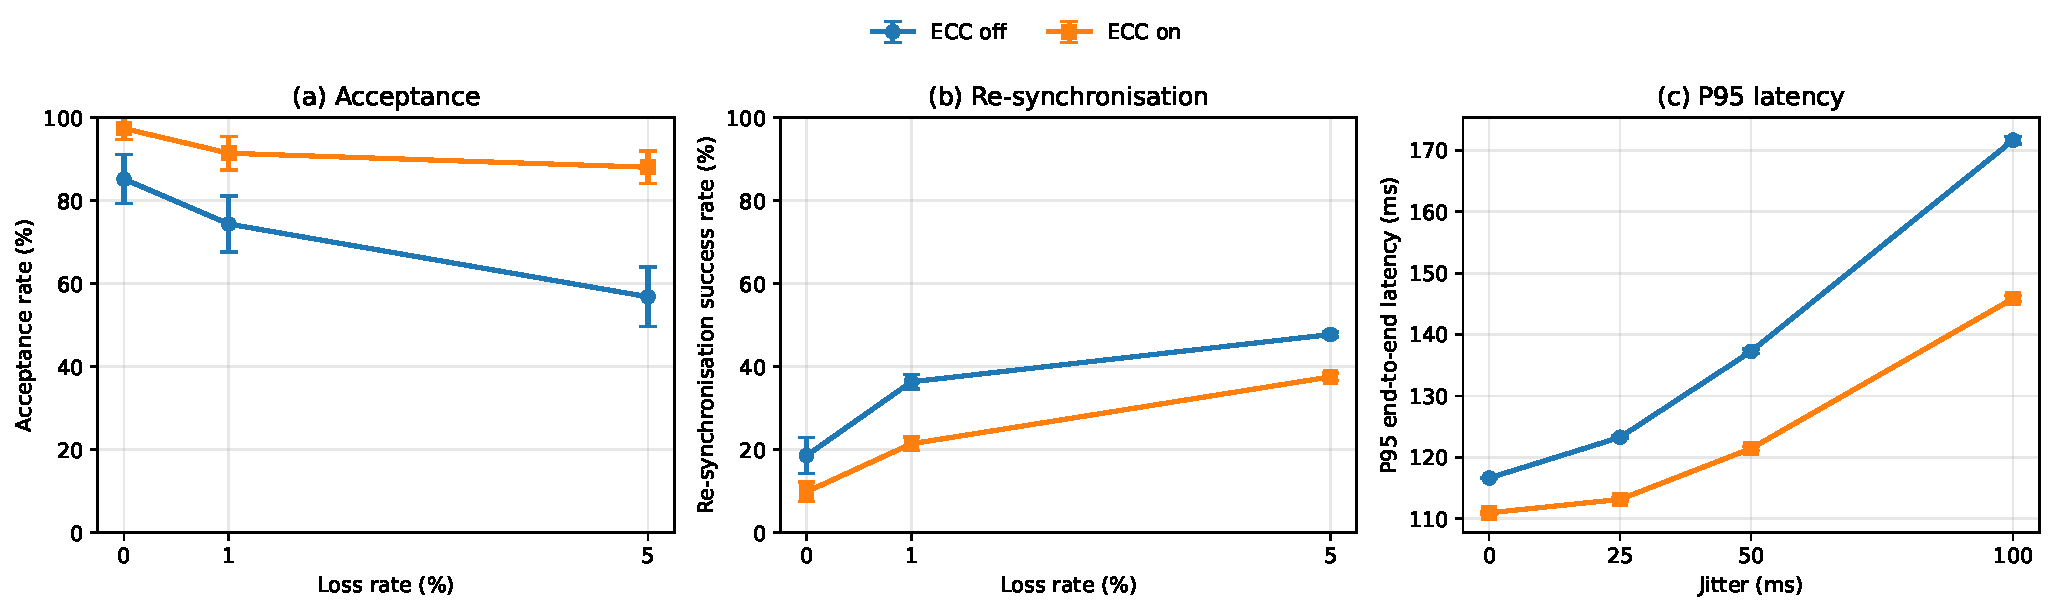
\includegraphics[width=\textwidth]{Figure_4.pdf}
    \caption{Synthetic transport simulation under controlled channel impairments. Panels show: (a) epoch acceptance rate under increasing channel loss, (b) re-synchronisation success rate under increasing channel loss, and (c) 95th-percentile end-to-end latency under increasing jitter. Results are shown for the configuration \(W=5\), \(h=10\), \(\Delta=100\) ms, and timeout \(2\Delta\); bars are descriptive 95\% t-based summary intervals across the selected
    settings and seeds, rather than population reliability bounds. The
    plotted subset has 480 unique parameter/seed scenarios.}
    \label{fig:qim_resync_combined}
\end{figure*}


\begin{table*}[!t]
\centering
\caption[Synthetic transport abstraction under channel loss. Results are reported as mean~$\pm$~standard deviation over unique parameter/seed scenarios, except false accepts, which are reported as total counts.]
{Synthetic transport abstraction under channel loss. Results are reported as mean~$\pm$~standard deviation over unique parameter/seed scenarios, except false accepts, which are reported as total counts.}
\label{tab:qim_resync_robustness}

\small
\setlength{\tabcolsep}{4.5pt}
\renewcommand{\arraystretch}{1.15}

\resizebox{\textwidth}{!}{%
\begin{threeparttable}

\begin{tabular}{
@{}
l
c
r
c
c
c
c
r
@{}}
\toprule
\textbf{Loss \boldmath$r$} &
\textbf{ECC} &
\textbf{Runs} &
\textbf{Acceptance (\%)} &
\textbf{Recovery (\%)} &
\textbf{Re-sync success (\%)} &
\textbf{Integrity fail (\%)} &
\textbf{False accepts} \\
\midrule
$0\%$ & Off & 4,320 & $82.25 \pm 30.68$ & $0.00 \pm 0.00$ & $20.69 \pm 22.55$ & $0.0000 \pm 0.0000$ & 0 \\
$0\%$ & On & 4,320 & $97.27 \pm 11.27$ & $61.31 \pm 7.27$ & $14.68 \pm 20.31$ & $0.0000 \pm 0.0000$ & 0 \\
$1\%$ & Off & 4,320 & $73.08 \pm 36.35$ & $0.00 \pm 0.00$ & $34.35 \pm 14.31$ & $0.0000 \pm 0.0000$ & 0 \\
$1\%$ & On & 4,320 & $88.11 \pm 24.76$ & $56.18 \pm 15.83$ & $24.73 \pm 17.78$ & $0.0000 \pm 0.0000$ & 0 \\
$5\%$ & Off & 4,320 & $53.41 \pm 36.22$ & $0.00 \pm 0.00$ & $44.88 \pm 7.91$ & $0.0000 \pm 0.0000$ & 0 \\
$5\%$ & On & 4,320 & $78.31 \pm 30.74$ & $51.96 \pm 20.40$ & $36.13 \pm 11.69$ & $0.0000 \pm 0.0000$ & 0 \\
\bottomrule
\end{tabular}

\begin{tablenotes}
\footnotesize
\item \textit{Notes:} These synthetic runs use an idealised erasure-recovery abstraction, not a concrete authenticated ECC decoder for the complete-epoch protocol. They do not validate whole-epoch integrity or image/plaintext recovery. ECC denotes the idealised erasure-recovery rule. Acceptance measures the proportion of epochs accepted after freshness, window, and MAC checks; recovery measures epochs reconstructed after partial channel loss; and re-sync success measures successful restoration of receiver alignment after incomplete or delayed epochs.
\end{tablenotes}

\end{threeparttable}%
}
\end{table*}



\begin{table*}[t]
\centering
\caption{Synthetic transport abstraction under channel jitter. Results are reported as mean~$\pm$~standard deviation over unique parameter/seed scenarios.}
\label{tab:qim_resync_latency}
\setlength{\tabcolsep}{5pt}
\renewcommand{\arraystretch}{1.15}
\resizebox{1.0\textwidth}{!}{%
\begin{tabular}{@{}llrcccc@{}}
\toprule
\textbf{Jitter (ms)} & \textbf{ECC} & \textbf{Runs} & \textbf{Mean Latency (ms)} & \textbf{P95 Latency (ms)} & \textbf{Mean Re-sync Delay (ms)} & \textbf{Throughput (epochs/s)} \\
\midrule
$0$ & Off & 3,240 & $80.21 \pm 32.94$ & $132.62 \pm 60.21$ & $83.18 \pm 23.07$ & $6.64 \pm 3.81$ \\
$0$ & On & 3,240 & $50.00 \pm 18.65$ & $126.03 \pm 56.70$ & $75.19 \pm 19.79$ & $8.75 \pm 2.52$ \\
$25$ & Off & 3,240 & $81.74 \pm 32.66$ & $139.30 \pm 57.43$ & $84.01 \pm 25.07$ & $7.12 \pm 3.59$ \\
$25$ & On & 3,240 & $50.48 \pm 18.44$ & $128.50 \pm 54.77$ & $75.64 \pm 19.75$ & $8.85 \pm 2.45$ \\
$50$ & Off & 3,240 & $85.00 \pm 31.37$ & $152.91 \pm 54.67$ & $84.27 \pm 22.15$ & $7.11 \pm 3.59$ \\
$50$ & On & 3,240 & $51.88 \pm 17.77$ & $136.60 \pm 51.56$ & $75.95 \pm 17.95$ & $8.83 \pm 2.45$ \\
$100$ & Off & 3,240 & $95.12 \pm 28.51$ & $184.94 \pm 52.41$ & $87.72 \pm 18.54$ & $6.96 \pm 3.62$ \\
$100$ & On & 3,240 & $56.76 \pm 15.95$ & $159.27 \pm 47.11$ & $78.18 \pm 15.40$ & $8.72 \pm 2.55$ \\
\bottomrule
\end{tabular}%
}
\par\medskip\noindent
\begin{minipage}{0.98\textwidth}
\footnotesize
\emph{Note:} These synthetic runs use an idealised erasure-recovery abstraction, not a concrete authenticated ECC decoder for the complete-epoch protocol. They do not validate whole-epoch integrity or image/plaintext recovery. ECC denotes the idealised erasure-recovery rule. Mean latency and P95 latency measure end-to-end epoch acceptance delay, while mean re-synchronisation delay measures the time required to restore receiver alignment after incomplete, delayed, or reordered channel observations.
\end{minipage}
\end{table*}

















\clearpage
\section{Native Generative and Distributed-Message Comparisons}
\label{sec:native-comparisons}

This section supplies the methodology and complete numerical tables for
the two native comparisons in main
Sections~\ref{main-subsec:native-pulsar} and
\ref{main-subsec:native-assemblage}. Both use the same CPM
protocol, receiver-reproducible masking path and fused weight 0.75.
The source snapshots, fixed inputs, native attempts, failures, models,
selection records and predictions are preserved. No failed native case
is retried or replaced. The completed matched HSMNet study at
0.10/0.20/0.40 bpp is reported separately in
Appendix~\ref{sec:hsmnet-comparison} and supplies no results to this
native-format panel.

\subsection{Common comparison and reproducibility rules}
\label{subsec:native-repro}
The common quantity is application-message bytes. CPM retains its
$512\times512$ 8-bit grayscale PGM carrier, two 65,536-byte public
parameter objects and three authenticated JSON/base64 frames. Pulsar
retains $256\times256$ RGB 16-bit lossless PNG carriers. Their benign
sources and protocol services differ; matching application bytes does
not make bpp, original-cover PSNR or network interfaces identical.
Undefined cross-channel CP-UNL scores for the native synthesis
interfaces are marked not applicable rather than assigned zero.
For CPM, the 128/256/384-byte grid corresponds to approximately
0.00391/0.00781/0.01172 application bpp; the distributed-message grid
corresponds to 0.03125/0.0625/0.125 bpp. These byte-matched panels
therefore do not replace the separate 0.10/0.20/0.40-bpp detector study.

The Pulsar source snapshot is commit
\texttt{52c263976770} of the official artifact
\cite{Jois2024Pulsar}. Assemblage uses official commit
\texttt{ce16a471ea0a} and its exact Pulsar submodule
\texttt{ae39c51440b5} \cite{Jois2026Assemblage}.
The generator is \texttt{google/ddpm-church-256}, pinned at revision
\texttt{5a1118b5a35e}, with native 50-step DDIM sampling
($\eta=1$), 100 histogram bins and one region estimate.
The run manifests contain complete commit identifiers and SHA-256
hashes of all frozen sources, configurations, model files and inputs.
Compatibility adapters change local model/temporary paths, inject
fixture keys through the supported native key configuration, and cast
equivalent NumPy Boolean values to integers for bit-array compatibility.
They do not change the native coding or model architecture.

The isolated comparison environment uses Python 3.12.14, PyTorch 2.12.0,
Diffusers 0.27.2, NumPy 2.4.5, scikit-learn 1.8.0,
\texttt{pystcstego} 0.1.0, \texttt{pdqhash} 0.2.8 and
\texttt{raptorq} 2.0.0, with SageMath 10.3/Python 3.10 for native
region coding. The workstation is specified in the main setup.
Model loading, region estimation, offline preparation, encoding and
decoding retain separate raw timing fields. Endpoint wall times below
include process/model overhead and shared-workstation contention;
they are descriptive measurements rather than an isolated speed ranking.

\subsection{Pulsar: generation, detector selection and uncertainty}
\label{subsec:native-pulsar-method}
The fixed panel comprises 200 source groups, each pairing a
BOSSBase cover with a native church-model seed. Groups are split
100/40/60 into training/validation/test; all methods and message
lengths of a group remain in the same split. Each group carries saved
messages of 128, 256 and 384 bytes, giving 600 attempts per method.
The independent native receiver initializes its own model/region path
and checks the recovered application bytes and padding. Capacity
shortfalls and native encoding/decoding failures remain in all-attempt
recovery counts. Original-cover PSNR/SSIM apply only to CPM.

Content detection uses the same fixed 504-dimensional native-precision
pixel, residual, quantile, bit-plane and cross-channel feature map for
both methods. CPM's benign examples are the source covers; Pulsar's
are unmodified outputs of the same sampler, using the same 16-bit
serialization as its stego images. Only image content enters a feature
vector: keys, seeds, original-cover differences, verification outcomes,
paths and hidden generation labels are excluded. A synthetic bit-plane
known-leak control using this feature map achieved AUC 1.0 for both
classifier families; it checks implementation sensitivity to that
planted signal rather than detector completeness.

Logistic regression uses training-only standardization,
$C\in\{0.01,0.1,1,10\}$ and a 4,000-iteration cap.
The ExtraTrees family averages three 500-tree models with seeds
901/902/903, minimum leaf size 2 and feature fraction 0.7.
Regularization, score orientation and the balanced-accuracy threshold
are selected using validation only. At each message length, a common
primary family for the two native sources is selected by their mean
validation AUC. Both families are retained in the reported diagnostics.
The held-out data are scored once after selection is frozen.

The detector panel includes a source group only if both native methods
recover its message exactly; the exclusion is symmetric and does not
alter all-attempt recovery denominators. Fixed minimum counts are
60 training, 24 validation and 36 test groups; no minimum is relaxed.
The resulting complete cohorts are in
Table~\ref{tab:native-cohorts}. Source-group bootstrap weights use
3,000 multinomial draws over the 60 held-out source groups with seed
61019; the same weights propagate each symmetric complete cohort and
both methods. Table~\ref{tab:native-detection} reports pointwise 95\%
intervals, while Table~\ref{tab:native-contrasts} uses percentile
endpoints $0.05/6$ and $1-0.05/6$ for the three primary payload
contrasts. These remain finite-observer comparisons, not numerical
values of the compositional security losses.

\subsection{Assemblage: local message path and erasure traces}
\label{subsec:native-assemblage-method}
Ten source/message groups at each of 1,024, 2,048 and 4,096 bytes
give 30 fixed messages per method. Assemblage retains native PDQ
discovery, offline state, region ECC and RaptorQ packetization with
MTU 408 bytes and 50\% additional repair packets. Candidate capacity
is checked using the original gate; insufficient candidates are
skipped, without replacement. The local receiver consumes actual
decoded packets. An exception in native carrier decoding aborts the
message as in the recorded upstream path; ground truth is never used
to filter decoded packets. This fixed one-pass panel does not add
offline trial-decoding selection or candidate regeneration.
Its failures therefore describe this configuration and do not imply
that Assemblage cannot improve delivery through other state-selection
or redundancy policies.

Each native carrier/frame is generated and decoded once. Saved
outcomes are replayed under fixed independent per-object erasure
probabilities $p\in\{0,0.1,0.2,0.3\}$ with seeds
2101--2105. A CPM object is one authenticated frame; an Assemblage
object is one image. The erasure law is shared, but object sizes and
counts differ. There is no byte-level network simulation or online
platform posting. Five seeds across 30 messages, four erasure levels
and two methods give 1,200 traces, not 1,200 independent messages.
At zero loss all five seeds reproduce the same intact outcome.

Delivery is summarized by averaging the five seed outcomes within a
source group and bootstrapping the ten source groups with 3,000 draws
and seed 61020. The pointwise intervals in
Table~\ref{tab:native-delivery} describe this small fixed cohort.
When all ten recorded groups succeed, percentile resampling gives
$[1,1]$; this boundary interval does not establish a zero population
failure probability. All traces had zero incorrect complete messages.
Across the candidate set, 71 of 310 packets were skipped for capacity
and 18 transmitted carriers produced native decoder exceptions
(Table~\ref{tab:native-failures}).

\subsection{Cost denominators and verification}
\label{subsec:native-cost-interpretation}
Table~\ref{tab:native-recovery} preserves every generative attempt.
The byte, endpoint-time and fidelity means in
Table~\ref{tab:native-cost} condition on exact recovery, with
denominators given in the recovery table. In contrast,
Table~\ref{tab:native-system-cost} gives transmitted-byte means over
all ten local distributed-message attempts per length, including
unsuccessful deliveries. Pre-shared state/hash-bank bytes are separate
from transmitted carriers; they are not counted as traffic or presumed
free. Sampler setup and offline preparation are distinct from online
send cost. These distinctions prevent a complete authenticated epoch
from being treated as the same service as a native image primitive.

All native image/packet hashes and recovered application bytes passed
independent checks. The Pulsar panel reproduced all 24 selected
checkpoint prediction sets; its twelve AUC/interval panels and three
adjusted contrasts were independently recomputed from saved scores.
The Assemblage panel independently replayed all 1,200 saved-packet
traces and reproduced all 24 delivery rates and intervals. No image
generation, model selection or held-out scoring was repeated during
these audits. Neither comparison recorded a CPM image with an absolute
pixel change exceeding one level. Their results support the specific
receiver, carrier and cost observations in the main paper; CP-UNL,
MC-ATTACK forgery losses and network scheduling retain their separate
definitions and evidence.

\begin{table*}[!t]
\centering\small
\caption{Complete source-group cohorts used symmetrically by the two native content detectors. Each group supplies one benign and one stego image per method.}
\label{tab:native-cohorts}
\setlength{\tabcolsep}{4pt}\renewcommand{\arraystretch}{1.12}
\begin{tabular}{lrrr}
\toprule
Bytes & Training & Validation & Test\\
\midrule
128 & 94 & 36 & 55\\
256 & 92 & 35 & 53\\
384 & 74 & 34 & 45\\
\bottomrule
\end{tabular}

\end{table*}

\begin{table*}[!t]
\centering\small
\caption{Native generative recovery: every attempt remains in the denominator.}
\label{tab:native-recovery}
\setlength{\tabcolsep}{4pt}\renewcommand{\arraystretch}{1.12}
\begin{tabular}{lrrrrr}
\toprule
Method & Bytes & Attempts & Exact & Capacity failures & Other failures\\
\midrule
CPM & 128 & 200 & 200 & 0 & 0\\
Pulsar & 128 & 200 & 185 & 7 & 8\\
CPM & 256 & 200 & 200 & 0 & 0\\
Pulsar & 256 & 200 & 180 & 8 & 12\\
CPM & 384 & 200 & 200 & 0 & 0\\
Pulsar & 384 & 200 & 153 & 39 & 8\\
\bottomrule
\end{tabular}
\par\smallskip\parbox{.97\textwidth}{\footnotesize No incorrect decoded application payload was recorded. A capacity or native encoding/decoding failure is an unsuccessful attempt, not a replaced case.}
\end{table*}

\begin{table*}[!t]
\centering\small
\caption{Native generative cost and fidelity means, conditioned on exact recovery. Byte costs are decimal kB; times are seconds.}
\label{tab:native-cost}
\setlength{\tabcolsep}{4pt}\renewcommand{\arraystretch}{1.12}
\begin{tabular}{lrrrrrrr}
\toprule
Method & Bytes & Exact $n$ & Wire (kB) & Sender (s) & Receiver (s) & PSNR (dB) & SSIM\\
\midrule
CPM & 128 & 200 & 525.066 & 3.202 & 0.220 & 80.94 & 0.99999918\\
Pulsar & 128 & 185 & 378.099 & 10.738 & 11.585 & -- & --\\
CPM & 256 & 200 & 525.066 & 3.197 & 0.219 & 77.89 & 0.99999826\\
Pulsar & 256 & 180 & 378.831 & 10.751 & 11.720 & -- & --\\
CPM & 384 & 200 & 525.066 & 3.201 & 0.222 & 76.00 & 0.99999722\\
Pulsar & 384 & 153 & 380.019 & 10.777 & 11.991 & -- & --\\
\bottomrule
\end{tabular}
\par\smallskip\parbox{.97\textwidth}{\footnotesize Sender/receiver times include process and model/region preparation where applicable. Pulsar has no original-cover PSNR/SSIM. CPM pure embedding means are 2.542/2.540/2.544 s at 128/256/384 bytes; these exclude epoch/process work and are not equivalent to native endpoint wall times.}
\end{table*}

\begin{table*}[!t]
\centering\small
\caption{Complete native-source content-detection diagnostics. P denotes the validation-selected primary family; all other rows remain secondary.}
\label{tab:native-detection}
\setlength{\tabcolsep}{4pt}\renewcommand{\arraystretch}{1.12}
\begin{tabular}{lrlcrlrr}
\toprule
Method & Bytes & Family & P & Test groups & AUC [95\% CI] & BAcc. & $\widehat\Delta$\\
\midrule
CPM & 128 & LR & yes & 55 & 0.5002 [0.4883, 0.5112] & 0.4909 & -0.0182\\
CPM & 128 & ET & -- & 55 & 0.5101 [0.4969, 0.5292] & 0.5091 & 0.0182\\
Pulsar & 128 & LR & yes & 55 & 0.5445 [0.4889, 0.6049] & 0.5182 & 0.0364\\
Pulsar & 128 & ET & -- & 55 & 0.4818 [0.3810, 0.5772] & 0.5182 & 0.0364\\
CPM & 256 & LR & -- & 53 & 0.5041 [0.4906, 0.5192] & 0.5000 & 0.0000\\
CPM & 256 & ET & yes & 53 & 0.5043 [0.4818, 0.5292] & 0.5094 & 0.0189\\
Pulsar & 256 & LR & -- & 53 & 0.4229 [0.3276, 0.5172] & 0.5000 & 0.0000\\
Pulsar & 256 & ET & yes & 53 & 0.5251 [0.4330, 0.6214] & 0.5660 & 0.1321\\
CPM & 384 & LR & yes & 45 & 0.4963 [0.4819, 0.5090] & 0.5111 & 0.0222\\
CPM & 384 & ET & -- & 45 & 0.4936 [0.4704, 0.5163] & 0.5000 & 0.0000\\
Pulsar & 384 & LR & yes & 45 & 0.6035 [0.5091, 0.6962] & 0.5111 & 0.0222\\
Pulsar & 384 & ET & -- & 45 & 0.4514 [0.3231, 0.5733] & 0.4444 & -0.1111\\
\bottomrule
\end{tabular}
\par\smallskip\parbox{.97\textwidth}{\footnotesize LR: logistic regression; ET: ExtraTrees ensemble. BAcc.: balanced accuracy at the validation-fixed threshold. The signed acceptance gap is $\widehat\Delta=\Pr[\widehat D=1\mid\mathrm{stego}]-\Pr[\widehat D=1\mid\mathrm{benign}]$ for this fixed rule, not a cryptographic advantage bound. Intervals are pointwise.}
\end{table*}

\begin{table*}[!t]
\centering\small
\caption{Primary paired AUC differences with three-payload adjusted percentile intervals.}
\label{tab:native-contrasts}
\setlength{\tabcolsep}{4pt}\renewcommand{\arraystretch}{1.12}
\begin{tabular}{rlrl}
\toprule
Bytes & Family & CPM minus Pulsar AUC & Adjusted interval\\
\midrule
128 & LR & -0.0443 & [-0.1244, 0.0287]\\
256 & ET & -0.0208 & [-0.1406, 0.0995]\\
384 & LR & -0.1072 & [-0.2239, 0.0092]\\
\bottomrule
\end{tabular}
\par\smallskip\parbox{.97\textwidth}{\footnotesize Every adjusted interval contains zero. In particular, the pointwise Pulsar 384-byte interval excludes chance in Table~\ref{tab:native-detection}, but the adjusted between-method contrast does not establish detectability superiority.}
\end{table*}

\begin{table*}[!t]
\centering\small
\caption{Complete local distributed-message delivery results. Each row has ten unique source groups and 50 recorded seed traces.}
\label{tab:native-delivery}
\setlength{\tabcolsep}{4pt}\renewcommand{\arraystretch}{1.12}
\begin{tabular}{lrrlr}
\toprule
Method & Bytes & Erasure $p$ & Exact rate [95\% CI] & Incorrect messages\\
\midrule
CPM & 1024 & 0.00 & 1.000 [1.000, 1.000] & 0\\
CPM & 1024 & 0.10 & 0.780 [0.700, 0.860] & 0\\
CPM & 1024 & 0.20 & 0.560 [0.420, 0.680] & 0\\
CPM & 1024 & 0.30 & 0.380 [0.240, 0.500] & 0\\
Assemblage & 1024 & 0.00 & 0.600 [0.300, 0.900] & 0\\
Assemblage & 1024 & 0.10 & 0.540 [0.280, 0.800] & 0\\
Assemblage & 1024 & 0.20 & 0.440 [0.220, 0.660] & 0\\
Assemblage & 1024 & 0.30 & 0.320 [0.140, 0.500] & 0\\
CPM & 2048 & 0.00 & 1.000 [1.000, 1.000] & 0\\
CPM & 2048 & 0.10 & 0.720 [0.620, 0.820] & 0\\
CPM & 2048 & 0.20 & 0.500 [0.360, 0.660] & 0\\
CPM & 2048 & 0.30 & 0.300 [0.180, 0.440] & 0\\
Assemblage & 2048 & 0.00 & 0.500 [0.200, 0.800] & 0\\
Assemblage & 2048 & 0.10 & 0.440 [0.180, 0.700] & 0\\
Assemblage & 2048 & 0.20 & 0.320 [0.100, 0.560] & 0\\
Assemblage & 2048 & 0.30 & 0.180 [0.000, 0.380] & 0\\
CPM & 4096 & 0.00 & 1.000 [1.000, 1.000] & 0\\
CPM & 4096 & 0.10 & 0.620 [0.560, 0.680] & 0\\
CPM & 4096 & 0.20 & 0.480 [0.360, 0.600] & 0\\
CPM & 4096 & 0.30 & 0.340 [0.260, 0.420] & 0\\
Assemblage & 4096 & 0.00 & 0.400 [0.100, 0.700] & 0\\
Assemblage & 4096 & 0.10 & 0.320 [0.100, 0.580] & 0\\
Assemblage & 4096 & 0.20 & 0.180 [0.040, 0.400] & 0\\
Assemblage & 4096 & 0.30 & 0.120 [0.020, 0.260] & 0\\
\bottomrule
\end{tabular}
\par\smallskip\parbox{.97\textwidth}{\footnotesize The 1,200 total traces reuse the same 30 fixed messages per method; they are not independent messages. Five zero-loss seeds repeat each intact outcome. Pointwise source-group percentile intervals can collapse at observed 10/10 success and do not establish population-perfect reliability.}
\end{table*}

\begin{table*}[!t]
\centering\small
\caption{Retained native Assemblage candidate and decoder outcomes before added erasures.}
\label{tab:native-failures}
\setlength{\tabcolsep}{4pt}\renewcommand{\arraystretch}{1.12}
\begin{tabular}{lrrrrr}
\toprule
Bytes & Candidates & Capacity skips & Sent carriers & Decoder exceptions & Intact recovery\\
\midrule
1024 & 50 & 14 & 36 & 3 & 6/10\\
2048 & 90 & 20 & 70 & 5 & 5/10\\
4096 & 170 & 37 & 133 & 10 & 4/10\\
\bottomrule
\end{tabular}
\par\smallskip\parbox{.97\textwidth}{\footnotesize Exceptions count carriers, not independent messages; different message-level failure causes can overlap. No candidate is regenerated or removed on the basis of ground-truth decoding.}
\end{table*}

\begin{table*}[!t]
\centering\small
\caption{Local distributed-message mean byte costs over all ten attempts per length, including failed deliveries. Units are decimal kB.}
\label{tab:native-system-cost}
\setlength{\tabcolsep}{4pt}\renewcommand{\arraystretch}{1.12}
\begin{tabular}{lrrrrr}
\toprule
Method & Bytes & Sent objects & Transmitted (kB) & State (kB) & Hash bank (kB)\\
\midrule
CPM & 1024 & 3.0 & 525.066 & -- & --\\
Assemblage & 1024 & 3.6 & 1360.283 & 28679.293 & 19.777\\
CPM & 2048 & 3.0 & 525.067 & -- & --\\
Assemblage & 2048 & 7.0 & 2663.186 & 51675.503 & 35.597\\
CPM & 4096 & 3.0 & 525.067 & -- & --\\
Assemblage & 4096 & 13.3 & 5056.740 & 97760.179 & 67.237\\
\bottomrule
\end{tabular}
\par\smallskip\parbox{.97\textwidth}{\footnotesize CPM traffic includes the public objects and authenticated frames. Assemblage state and hash banks are pre-shared setup artifacts, separate from traffic. Dashes denote a non-equivalent/unreported native interface, not a claim of zero setup cost.}
\end{table*}

\begin{table*}[!t]
\centering\small
\caption{Local distributed-message mean timing components over all ten attempts per length, in seconds.}
\label{tab:native-system-time}
\setlength{\tabcolsep}{4pt}\renewcommand{\arraystretch}{1.12}
\begin{tabular}{lrrrrrr}
\toprule
Method & Bytes & Sender wall & Receiver wall & Offline & Native send & Native pipeline\\
\midrule
CPM & 1024 & 2.972 & 0.185 & -- & -- & --\\
Assemblage & 1024 & -- & -- & 29.815 & 6.241 & 48.579\\
CPM & 2048 & 2.967 & 0.195 & -- & -- & --\\
Assemblage & 2048 & -- & -- & 53.019 & 12.093 & 87.311\\
CPM & 4096 & 2.965 & 0.200 & -- & -- & --\\
Assemblage & 4096 & -- & -- & 99.544 & 23.264 & 162.212\\
\bottomrule
\end{tabular}
\par\smallskip\parbox{.97\textwidth}{\footnotesize The native pipeline is the recorded Assemblage local offline/send/receive process; its components and CPM endpoint wall times are different boundaries. Measurements include shared-workstation contention, so these columns must not be read as an isolated equal-service speed benchmark.}
\end{table*}


\clearpage
\section{Matched Five-Method Image-Carrier and HSMNet Evaluation}
\label{sec:hsmnet-comparison}
This appendix supports main-text Sections~\ref{main-subsec:setup},
\ref{main-subsec:embedding_fidelity} and
\ref{main-subsec:hsmnet-comparison}, including
Fig.~\ref{main-fig:matched-hsmnet}. It reports the completed image-only
comparison of the \texttt{cpm-epoch-v2} carrier with recorded
S-UNIWARD, MiPOD, WOW and HILL implementations. The local MiPOD variance
estimator is an approximation, denoted MiPOD$^\dagger$ in every table.
These are implementation-specific comparisons, not certified upstream
reference-code rankings. They neither evaluate the full public view nor
assign a CP-UNL score to a single-carrier primitive; that evidence remains
in main-text Section~\ref{main-sec:empirical_linkability}.

\subsection{Cohorts, implementations and retained attempts}
The original 1,200 cover identities retain their 700/200/300
training/validation/test partitions. Each identity contributes at most
one image per method and application payload (0.10/0.20/0.40 bpp), yielding
18,000 retained records: 3,600 CPM attempts and 14,400 reused
baseline records. All images are native $512\times512$ grayscale
BOSSBase images. The baseline records use keyed pseudorandom payloads
with the same net lengths and recorded byte/header padding as the CPM
comparison, but their message bytes are different. No saved baseline
image was regenerated. The local source snapshots and original run
identifiers are listed in Table~\ref{tab:hsm-versions}; complete SHA-256
manifests accompany the saved artifacts. The native STC interface is
\texttt{pystcstego}~0.1.0. CPM uses the receiver-reproducible mask and
authenticated epoch binding, whereas the baseline primitives embed their
messages directly and supply no corresponding public-parameter or
authentication service.

Every detector/fidelity block must contain valid images for all five
methods on the same cover and payload. Incomplete blocks are excluded
symmetrically, without replacement, from these conditional comparisons;
every attempt remains in the separate totals. Table~\ref{tab:hsm-cohorts}
gives the realised common-valid counts, exceeding the fixed minimum
600/150/240 train/validation/test counts at each payload.
Tables~\ref{tab:hsm-accounting} and \ref{tab:hsm-images} retain all 111
invalid image records. CPM exact recovery and authentication were
independently checked for 3,595 of 3,600 attempts. For the reused baseline
records, valid images and source-reported extraction success do not
establish independent recovery of the original unavailable message
bytes. The separate known-message panel below supplies those checks.
One retained main-panel HILL image has an absolute pixel change exceeding
one level; no CPM image does. It was not removed from the valid-image
panel. No fresh-panel image has such a deviation.

\subsection{Frozen HSMNet training and validation-only choices}
The official HSMNet architecture \cite{Yang2026HSMNet}, commit
\texttt{2c9f57be9c24753308931ee7e016c9cb2958813d}, is unchanged. Six
models (three payloads, seeds 801 and 802) each complete the fixed
100-epoch schedule in Table~\ref{tab:hsm-config}. Each payload/seed has
one equal-method mixture observer, shared across the five methods, rather
than a separately optimised detector per method. For training cover index
$i$ at epoch $e$ and seed $s$, the method cycles as $(i+e+s)\bmod5$ in
the order CPM, S-UNIWARD, MiPOD$^\dagger$, WOW, HILL. Training cover and
stego images receive the same random dihedral transformation. Checkpoint
selection minimises equal-method mean validation cross-entropy at epoch
1 and every five epochs thereafter. The two selected seed logit
differences are averaged, after which a common orientation and
balanced-error threshold are fixed using validation only
(Table~\ref{tab:hsm-thresholds}). One frozen held-out scoring pass gives
the fifteen method/payload panels. No test-based tuning, early stopping,
new model, repeated selection or failed-trial replacement is used.
This declared budget is not a reproduction of HSMNet's published
training protocol or benchmark scores. Its scope is the shared image
observer trained here; it is not a comparison of independently optimised
best-possible wardens for each method.

\subsection{Uncertainty, complete results and interpretation}
The uncertainty unit is source-cover identity, preserving each
cover/stego pair and the dependence across methods and payloads. With
seed 61018, 3,000 bootstrap draws sample the 300 test source identities
with replacement and then restrict to common-valid blocks for each
payload. The same draws are shared across all methods and payloads.
The 2.5th and 97.5th percentiles give the pointwise 95\% intervals in
Table~\ref{tab:hsm-detection}. For twelve CPM-minus-baseline AUC
contrasts (four baselines, three payloads), the adjusted endpoints use
quantiles $0.05/(2\cdot12)$ and $1-0.05/(2\cdot12)$, retaining the fixed
Bonferroni family convention (Table~\ref{tab:hsm-contrasts}). The same
twelve-comparison adjustment is applied separately within each fidelity
metric in Table~\ref{tab:hsm-fidelity-contrasts}; it is not a single
36-contrast family claim. Fidelity means and intervals use the identical
common-valid covers (Tables~\ref{tab:hsm-fidelity} and
\ref{tab:hsm-modifications}).

These percentile intervals condition on the saved models, validation
choices and valid-image cohort; they do not include training-seed or
model-fitting variability. Some low-payload intervals are asymmetric and
exclude their point estimate. The independently checked endpoints are
retained without clipping or widening. All fifteen pointwise AUC
intervals lie above 0.5. Numerically near-chance AUCs therefore cannot be
described as no detection or as equivalence. Seven adjusted relative
contrasts favour CPM: WOW at every payload, MiPOD$^\dagger$ at every
payload, and S-UNIWARD at 0.40 bpp. Five intervals include zero, including
all HILL comparisons. The MiPOD$^\dagger$ and S-UNIWARD advantages are
small in absolute AUC units. These results inform the empirical
image-carrier component $\varepsilon_{\mathsf{emb}}$ in main-text
Eq.~\eqref{main-eq:revised-composition}; AUC is not a cryptographic loss
estimate, and the intervals do not upper-bound the optimal warden.

\subsection{Known-message recovery, timing and byte costs}
Thirty fixed development covers, three payloads and five methods give
450 sequential known-message attempts, separate from held-out detector
selection. Saved message bytes permit independent native extraction and,
for CPM, authenticated receiver verification. CPM, S-UNIWARD,
MiPOD$^\dagger$ and WOW each recover 90/90 exactly; HILL recovers 86/90.
All four HILL failures return payloads that differ from the known message.
These are failed native extractions, not successful deliveries; the
single-carrier baselines have no CPM authentication/acceptance interface.
No incorrect plaintext is released by the CPM receiver.
Tables~\ref{tab:hsm-fresh-sender}--\ref{tab:hsm-fresh-bytes} give every
saved timing/byte summary. Mean and median costs condition on exact
recovery, with explicit denominators; they are not all-attempt latency
estimates. Core embedding consistently means cost-map computation plus
native STC embedding, excluding image serialisation. For the baselines
this is reconstructed from saved \texttt{cost\_sec + stc\_sec}; the raw
worker \texttt{core\_sec} also included image saving. The versioned
report-quality pass preserves the raw measurements and backs up the
corrected table. CPM core time is approximately 2.30 s, compared with
0.90--0.91 s for S-UNIWARD/WOW, 0.54--0.55 s for HILL and 3.24--3.25 s
for MiPOD$^\dagger$. These shared-workstation timings have different
protocol services and do not establish overall system superiority.
Missing baseline protocol-wire metrics are inapplicable, not zero.

\subsection{Checkpoint continuation and independent verification}
During the first payload/seed model, execution was interrupted in an
uncheckpointed portion of epoch 27. The versioned
\texttt{resume\_20261021\_v1} continuation restored the durable epoch-26
model, Adamax state and scheduler. Completed epochs 1--26 were retained
without retraining; only unsaved partial-epoch updates were discarded.
The original checkpoint omitted random-number-generator state. Fixed-seed
CPU/CUDA state was reconstructed using only the known dropout random
calls on constant feature-shaped tensors and validation-loader seed
draws, without replaying native image forward passes or gradients.
Subsequent last checkpoints saved CPU/CUDA state atomically. This is an
operational continuation with unchanged architecture, data, augmentation,
optimiser, schedule, 100-epoch budget, selection and uncertainty settings;
no held-out selection had occurred before interruption. Original source,
status, logs, model/history files and before/after hashes remain archived
with the continuation provenance.

The saved-artifact verifier reproduced all six selected checkpoint
prediction sets (absolute/relative tolerance $10^{-5}$) and all fifteen
two-seed ensembles, checked native CPM recovery/authentication, and
verified source/input/image/prediction hashes. An independent saved-score
audit reproduced all fifteen AUC/pointwise-interval panels, twelve
adjusted AUC contrasts, 45 fidelity mean/interval checks, 36 fidelity
contrasts and fifteen fresh recovery/cost summaries. The versioned
\texttt{report\_quality\_v1} pass corrected only saved baseline timing
aggregation and exposed retained pixel deviations. The final
\texttt{checked\_review\_v1} provenance retains exact before/after report
hashes. No image generation, training or test selection was repeated for
report preparation. These operational details do not alter the
separate full-public-view CP-UNL evidence in main-text
Section~\ref{main-sec:empirical_linkability}.

\begin{table*}[!t]
\centering\footnotesize
\caption{Fixed HSMNet configuration; the architecture is unchanged.}
\label{tab:hsm-config}
\setlength{\tabcolsep}{4pt}\renewcommand{\arraystretch}{1.15}
\begin{tabular}{lp{.73\textwidth}}
\toprule
Setting & Value\\
\midrule
Input & Native $512\times512$ grayscale; float values in $[0,255]$; no resizing\\
Training augmentation & Paired random dihedral (D4) transformations\\
Models / budget & Three payloads; seeds 801/802; six models; 100 fixed epochs each\\
Batch / data loading & Two cover--stego pairs (four images); two workers\\
Optimiser & Adamax; initial rate 0.001; $\epsilon=10^{-8}$; weight decay 0\\
Schedule & Milestones 60/85; multiplicative decay 0.1\\
Validation / selection & Epoch 1 and every five epochs; minimum joint validation cross-entropy\\
Ensemble / operating point & Mean of two seed logit differences; validation-only orientation/threshold\\
Uncertainty & Seed 61018; 3,000 shared test-cover bootstrap draws; fixed-model intervals\\
\bottomrule
\end{tabular}

\end{table*}

\begin{table*}[!t]
\centering\footnotesize
\caption{Implementation/version labels for the matched image panel.}
\label{tab:hsm-versions}
\setlength{\tabcolsep}{4pt}\renewcommand{\arraystretch}{1.15}
\begin{tabular}{lp{.76\textwidth}}
\toprule
Method & Recorded source\\
\midrule
CPM & \texttt{cpm-epoch-v2}; complete-epoch native carrier and receiver\\
S-UNIWARD & \texttt{suniward-20260520T013058-7be1b7}; local implementation\\
MiPOD$^\dagger$ & \texttt{mipod-20260521T042407-4584e4}; local variance approximation\\
WOW & \texttt{wow-20260519T024439-fbfdff}; local implementation\\
HILL & \texttt{hill-20260527T102926-77753a}; local implementation\\
\bottomrule
\end{tabular}
\par\smallskip\parbox{.97\textwidth}{\footnotesize $\dagger$: the local MiPOD variance approximation is retained throughout; none of the local baseline results is certified as an upstream reference-code result.}
\end{table*}

\begin{table*}[!t]
\centering\footnotesize
\caption{Five-method common-valid source-cover counts.}
\label{tab:hsm-cohorts}
\setlength{\tabcolsep}{4pt}\renewcommand{\arraystretch}{1.15}
\begin{tabular}{rrrrl}
\toprule
bpp & Train & Validation & Test & Original split\\
\midrule
0.10 & 681 & 195 & 288 & 700/200/300\\
0.20 & 684 & 196 & 289 & 700/200/300\\
0.40 & 671 & 195 & 294 & 700/200/300\\
\bottomrule
\end{tabular}

\end{table*}

\begin{table*}[!t]
\centering\footnotesize
\caption{All-attempt main image and fresh known-message accounting.}
\label{tab:hsm-accounting}
\setlength{\tabcolsep}{4pt}\renewcommand{\arraystretch}{1.15}
\begin{tabular}{lrrrrr}
\toprule
Method & Main attempts & Valid images & Invalid & Fresh exact/attempts & Pixel deviations\\
\midrule
CPM & 3600 & 3595 & 5 & 90/90 & 0\\
S-UNIWARD & 3600 & 3600 & 0 & 90/90 & 0\\
MiPOD$^\dagger$ & 3600 & 3600 & 0 & 90/90 & 0\\
WOW & 3600 & 3565 & 35 & 90/90 & 0\\
HILL & 3600 & 3529 & 71 & 86/90 & 1\\
\bottomrule
\end{tabular}
\par\smallskip\parbox{.97\textwidth}{\footnotesize Main CPM independent recovery/authentication: 3,595/3,600; original baseline message-byte recovery is not independently established. Pixel-deviation counts refer to retained main images with an absolute pixel change above one; fresh counts are all zero. No failed attempt is replaced.}
\end{table*}

\begin{table*}[!t]
\centering\footnotesize
\caption{Per-payload retained main image attempts across all three partitions.}
\label{tab:hsm-images}
\setlength{\tabcolsep}{4pt}\renewcommand{\arraystretch}{1.15}
\begin{tabular}{lrrrr}
\toprule
Method & bpp & Attempted & Valid & Invalid\\
\midrule
CPM & 0.10 & 1200 & 1199 & 1\\
S-UNIWARD & 0.10 & 1200 & 1200 & 0\\
MiPOD$^\dagger$ & 0.10 & 1200 & 1200 & 0\\
WOW & 0.10 & 1200 & 1184 & 16\\
HILL & 0.10 & 1200 & 1178 & 22\\
CPM & 0.20 & 1200 & 1197 & 3\\
S-UNIWARD & 0.20 & 1200 & 1200 & 0\\
MiPOD$^\dagger$ & 0.20 & 1200 & 1200 & 0\\
WOW & 0.20 & 1200 & 1192 & 8\\
HILL & 0.20 & 1200 & 1180 & 20\\
CPM & 0.40 & 1200 & 1199 & 1\\
S-UNIWARD & 0.40 & 1200 & 1200 & 0\\
MiPOD$^\dagger$ & 0.40 & 1200 & 1200 & 0\\
WOW & 0.40 & 1200 & 1189 & 11\\
HILL & 0.40 & 1200 & 1171 & 29\\
\bottomrule
\end{tabular}

\end{table*}

\begin{table*}[!t]
\centering\footnotesize
\caption{Validation-fixed common score orientations and thresholds.}
\label{tab:hsm-thresholds}
\setlength{\tabcolsep}{4pt}\renewcommand{\arraystretch}{1.15}
\begin{tabular}{rrr}
\toprule
bpp & Orientation & Threshold\\
\midrule
0.10 & 1 & -0.038325619\\
0.20 & 1 & 0.001119715\\
0.40 & 1 & -0.146289110\\
\bottomrule
\end{tabular}
\par\smallskip\parbox{.97\textwidth}{\footnotesize The same averaged-seed score orientation and threshold apply to all five methods at each payload.}
\end{table*}

\begin{table*}[!t]
\centering\footnotesize
\caption{Complete held-out HSMNet results with pointwise conditional 95\% intervals.}
\label{tab:hsm-detection}
\setlength{\tabcolsep}{4pt}\renewcommand{\arraystretch}{1.15}
\begin{tabular}{lrrlrr}
\toprule
Method & bpp & $n$ & AUC [interval] & Balanced accuracy & Signed gap $\widehat\Delta$\\
\midrule
CPM & 0.10 & 288 & 0.502423 [0.502665, 0.504315] & 0.503472 & 0.006944\\
S-UNIWARD & 0.10 & 288 & 0.503243 [0.503472, 0.505413] & 0.503472 & 0.006944\\
MiPOD$^\dagger$ & 0.10 & 288 & 0.503303 [0.503894, 0.505501] & 0.503472 & 0.006944\\
WOW & 0.10 & 288 & 0.522413 [0.521486, 0.527029] & 0.510417 & 0.020833\\
HILL & 0.10 & 288 & 0.502532 [0.502653, 0.504423] & 0.503472 & 0.006944\\
CPM & 0.20 & 289 & 0.505418 [0.505761, 0.507981] & 0.503460 & 0.006920\\
S-UNIWARD & 0.20 & 289 & 0.506268 [0.506643, 0.508984] & 0.505190 & 0.010381\\
MiPOD$^\dagger$ & 0.20 & 289 & 0.506352 [0.506853, 0.509087] & 0.506920 & 0.013841\\
WOW & 0.20 & 289 & 0.520085 [0.519309, 0.524480] & 0.512111 & 0.024221\\
HILL & 0.20 & 289 & 0.505669 [0.505928, 0.508250] & 0.503460 & 0.006920\\
CPM & 0.40 & 294 & 0.517007 [0.515892, 0.521747] & 0.505102 & 0.010204\\
S-UNIWARD & 0.40 & 294 & 0.519888 [0.518541, 0.524794] & 0.505102 & 0.010204\\
MiPOD$^\dagger$ & 0.40 & 294 & 0.518592 [0.517368, 0.523597] & 0.505102 & 0.010204\\
WOW & 0.40 & 294 & 0.582917 [0.575744, 0.593414] & 0.549320 & 0.098639\\
HILL & 0.40 & 294 & 0.517180 [0.515871, 0.522184] & 0.505102 & 0.010204\\
\bottomrule
\end{tabular}
\par\smallskip\parbox{.97\textwidth}{\footnotesize $\widehat\Delta=\Pr[\widehat D=1\mid\mathrm{stego}]-\Pr[\widehat D=1\mid\mathrm{cover}]$ for the validation-fixed rule. These fixed-rule values and AUCs are distinct quantities and are not upper bounds on $\varepsilon_{\mathsf{emb}}$. Percentile intervals may exclude the estimate.}
\end{table*}

\begin{table*}[!t]
\centering\footnotesize
\caption{All twelve CPM-minus-baseline AUC contrasts and family-adjusted intervals.}
\label{tab:hsm-contrasts}
\setlength{\tabcolsep}{4pt}\renewcommand{\arraystretch}{1.15}
\begin{tabular}{lrrl}
\toprule
Baseline & bpp & Difference & Adjusted interval\\
\midrule
S-UNIWARD & 0.10 & -0.000820 & [-0.002038, 0.000224]\\
MiPOD$^\dagger$ & 0.10 & -0.000880 & [-0.002283, -0.000206]\\
WOW & 0.10 & -0.019989 & [-0.024885, -0.016911]\\
HILL & 0.10 & -0.000109 & [-0.001116, 0.001045]\\
S-UNIWARD & 0.20 & -0.000850 & [-0.001985, 0.000054]\\
MiPOD$^\dagger$ & 0.20 & -0.000934 & [-0.002058, -0.000305]\\
WOW & 0.20 & -0.014667 & [-0.018641, -0.011937]\\
HILL & 0.20 & -0.000251 & [-0.001283, 0.000783]\\
S-UNIWARD & 0.40 & -0.002881 & [-0.004238, -0.001783]\\
MiPOD$^\dagger$ & 0.40 & -0.001585 & [-0.002618, -0.000846]\\
WOW & 0.40 & -0.065910 & [-0.078896, -0.054798]\\
HILL & 0.40 & -0.000174 & [-0.001201, 0.000772]\\
\bottomrule
\end{tabular}
\par\smallskip\parbox{.97\textwidth}{\footnotesize Negative differences favour CPM for the fixed validation-oriented observer. Seven intervals are below zero; five include zero.}
\end{table*}

\begin{table*}[!t]
\centering\footnotesize
\caption{Matched test-cover fidelity means and pointwise 95\% intervals.}
\label{tab:hsm-fidelity}
\setlength{\tabcolsep}{4pt}\renewcommand{\arraystretch}{1.15}
\begin{tabular}{lrrll}
\toprule
Method & bpp & $n$ & PSNR (dB) [interval] & SSIM [interval]\\
\midrule
CPM & 0.10 & 288 & 65.672 [65.623, 65.719] & 0.99994765 [0.99994299, 0.99995228]\\
S-UNIWARD & 0.10 & 288 & 65.935 [65.879, 65.990] & 0.99993711 [0.99993188, 0.99994234]\\
MiPOD$^\dagger$ & 0.10 & 288 & 66.143 [66.095, 66.191] & 0.99992720 [0.99992179, 0.99993255]\\
WOW & 0.10 & 288 & 65.052 [64.994, 65.109] & 0.99971775 [0.99971010, 0.99972525]\\
HILL & 0.10 & 288 & 65.415 [65.335, 65.495] & 0.99993052 [0.99992458, 0.99993628]\\
CPM & 0.20 & 289 & 62.211 [62.165, 62.257] & 0.99985522 [0.99984335, 0.99986708]\\
S-UNIWARD & 0.20 & 289 & 62.548 [62.498, 62.600] & 0.99983214 [0.99981974, 0.99984473]\\
MiPOD$^\dagger$ & 0.20 & 289 & 62.432 [62.374, 62.489] & 0.99981967 [0.99980677, 0.99983306]\\
WOW & 0.20 & 289 & 61.689 [61.630, 61.746] & 0.99940232 [0.99938506, 0.99941940]\\
HILL & 0.20 & 289 & 62.008 [61.934, 62.083] & 0.99981779 [0.99980370, 0.99983219]\\
CPM & 0.40 & 294 & 58.660 [58.620, 58.699] & 0.99959495 [0.99956499, 0.99962531]\\
S-UNIWARD & 0.40 & 294 & 59.028 [58.984, 59.071] & 0.99955260 [0.99952219, 0.99958329]\\
MiPOD$^\dagger$ & 0.40 & 294 & 58.554 [58.493, 58.617] & 0.99954082 [0.99950756, 0.99957427]\\
WOW & 0.40 & 294 & 58.170 [58.109, 58.229] & 0.99870778 [0.99866559, 0.99874902]\\
HILL & 0.40 & 294 & 58.503 [58.433, 58.570] & 0.99951844 [0.99948321, 0.99955357]\\
\bottomrule
\end{tabular}
\par\smallskip\parbox{.97\textwidth}{\footnotesize Every row uses the same common-valid test covers across methods within a payload. Fidelity is conditional on valid images.}
\end{table*}

\begin{table*}[!t]
\centering\footnotesize
\caption{Modified-pixel means and pointwise intervals, with separate per-method test validity.}
\label{tab:hsm-modifications}
\setlength{\tabcolsep}{4pt}\renewcommand{\arraystretch}{1.15}
\begin{tabular}{lrrrl}
\toprule
Method & bpp & Common $n$ & Test valid/attempts & Modified pixels [interval]\\
\midrule
CPM & 0.10 & 288 & 300/300 & 4639.84 [4587.20, 4694.17]\\
S-UNIWARD & 0.10 & 288 & 300/300 & 4373.68 [4317.74, 4431.48]\\
MiPOD$^\dagger$ & 0.10 & 288 & 300/300 & 4162.80 [4114.70, 4211.55]\\
WOW & 0.10 & 288 & 297/300 & 5363.94 [5287.06, 5442.27]\\
HILL & 0.10 & 288 & 291/300 & 4965.56 [4872.22, 5061.43]\\
CPM & 0.20 & 289 & 298/300 & 10289.94 [10177.54, 10405.09]\\
S-UNIWARD & 0.20 & 289 & 300/300 & 9530.77 [9414.18, 9644.51]\\
MiPOD$^\dagger$ & 0.20 & 289 & 300/300 & 9803.15 [9667.68, 9940.77]\\
WOW & 0.20 & 289 & 296/300 & 11631.44 [11471.76, 11799.42]\\
HILL & 0.20 & 289 & 295/300 & 10865.00 [10673.73, 11060.52]\\
CPM & 0.40 & 294 & 300/300 & 23284.45 [23070.64, 23502.66]\\
S-UNIWARD & 0.40 & 294 & 300/300 & 21405.09 [21190.37, 21624.67]\\
MiPOD$^\dagger$ & 0.40 & 294 & 300/300 & 23974.46 [23620.43, 24325.11]\\
WOW & 0.40 & 294 & 300/300 & 26164.08 [25797.57, 26556.16]\\
HILL & 0.40 & 294 & 294/300 & 24293.14 [23908.21, 24693.22]\\
\bottomrule
\end{tabular}
\par\smallskip\parbox{.97\textwidth}{\footnotesize Test valid/attempts counts are per method; common-valid means use their intersection. Modified pixels count all nonzero pixel differences, including retained deviations larger than one.}
\end{table*}

\begin{table*}[!t]
\centering\scriptsize
\caption{All 36 paired fidelity contrasts: CPM minus baseline with adjusted intervals.}
\label{tab:hsm-fidelity-contrasts}
\setlength{\tabcolsep}{4pt}\renewcommand{\arraystretch}{1.15}
\begin{tabular}{lrlll}
\toprule
Baseline & bpp & $\Delta$PSNR (dB) & $10^5\Delta$SSIM & $\Delta$modified pixels\\
\midrule
S-UNIWARD & 0.10 & -0.263 [-0.324, -0.208] & 1.054 [0.858, 1.267] & 266.16 [210.94, 326.77]\\
MiPOD$^\dagger$ & 0.10 & -0.471 [-0.514, -0.427] & 2.045 [1.849, 2.251] & 477.04 [431.21, 525.10]\\
WOW & 0.10 & 0.620 [0.509, 0.731] & 22.990 [21.695, 24.299] & -724.10 [-867.62, -587.21]\\
HILL & 0.10 & 0.257 [0.181, 0.334] & 1.713 [1.433, 2.012] & -325.72 [-417.77, -238.09]\\
S-UNIWARD & 0.20 & -0.337 [-0.392, -0.287] & 2.308 [1.915, 2.719] & 759.17 [643.93, 884.32]\\
MiPOD$^\dagger$ & 0.20 & -0.221 [-0.267, -0.177] & 3.555 [3.207, 3.925] & 486.80 [380.80, 597.82]\\
WOW & 0.20 & 0.522 [0.410, 0.627] & 45.290 [42.434, 48.293] & -1341.50 [-1617.48, -1036.72]\\
HILL & 0.20 & 0.203 [0.130, 0.270] & 3.743 [3.190, 4.278] & -575.06 [-748.35, -396.55]\\
S-UNIWARD & 0.40 & -0.368 [-0.411, -0.326] & 4.236 [3.467, 5.011] & 1879.36 [1659.77, 2103.39]\\
MiPOD$^\dagger$ & 0.40 & 0.105 [0.054, 0.158] & 5.413 [4.737, 6.188] & -690.01 [-1004.42, -390.96]\\
WOW & 0.40 & 0.490 [0.390, 0.584] & 88.717 [82.105, 95.477] & -2879.63 [-3470.54, -2281.49]\\
HILL & 0.40 & 0.157 [0.095, 0.216] & 7.651 [6.484, 9.041] & -1008.69 [-1367.57, -652.31]\\
\bottomrule
\end{tabular}
\par\smallskip\parbox{.97\textwidth}{\footnotesize Twelve-way adjustment is applied separately within each metric. Positive PSNR/SSIM differences favour CPM; fewer modified pixels alone do not establish lower detectability. SSIM differences and interval endpoints are multiplied by $10^5$ for legibility.}
\end{table*}

\begin{table*}[!t]
\centering\footnotesize
\caption{Known-message recovery and sender times; times are mean / median seconds over exact recoveries.}
\label{tab:hsm-fresh-sender}
\setlength{\tabcolsep}{4pt}\renewcommand{\arraystretch}{1.15}
\begin{tabular}{lrrrrll}
\toprule
Method & bpp & Exact/attempts & Failed & Mismatches & Core embedding & Sender wall\\
\midrule
CPM & 0.10 & 30/30 & 0 & 0 & 2.3006 / 2.2970 & 2.7696 / 2.7474\\
S-UNIWARD & 0.10 & 30/30 & 0 & 0 & 0.9023 / 0.8970 & 2.3797 / 2.3805\\
MiPOD$^\dagger$ & 0.10 & 30/30 & 0 & 0 & 3.2526 / 3.2652 & 3.7639 / 3.7743\\
WOW & 0.10 & 30/30 & 0 & 0 & 0.9081 / 0.9045 & 2.3985 / 2.4013\\
HILL & 0.10 & 27/30 & 3 & 3 & 0.5435 / 0.5396 & 2.0258 / 2.0168\\
CPM & 0.20 & 30/30 & 0 & 0 & 2.2966 / 2.2903 & 2.7646 / 2.7518\\
S-UNIWARD & 0.20 & 30/30 & 0 & 0 & 0.9040 / 0.9030 & 2.3846 / 2.3740\\
MiPOD$^\dagger$ & 0.20 & 30/30 & 0 & 0 & 3.2441 / 3.2563 & 3.7565 / 3.7668\\
WOW & 0.20 & 30/30 & 0 & 0 & 0.9131 / 0.9059 & 2.4005 / 2.4072\\
HILL & 0.20 & 30/30 & 0 & 0 & 0.5504 / 0.5427 & 2.0460 / 2.0496\\
CPM & 0.40 & 30/30 & 0 & 0 & 2.3021 / 2.3056 & 2.7788 / 2.7811\\
S-UNIWARD & 0.40 & 30/30 & 0 & 0 & 0.9082 / 0.9086 & 2.3844 / 2.3784\\
MiPOD$^\dagger$ & 0.40 & 30/30 & 0 & 0 & 3.2512 / 3.2463 & 3.7602 / 3.7579\\
WOW & 0.40 & 30/30 & 0 & 0 & 0.9088 / 0.9066 & 2.3921 / 2.3867\\
HILL & 0.40 & 29/30 & 1 & 1 & 0.5468 / 0.5371 & 2.0283 / 2.0407\\
\bottomrule
\end{tabular}
\par\smallskip\parbox{.97\textwidth}{\footnotesize Core embedding excludes serialisation and uses saved cost-map plus STC times. Each row attempts the same 30 development covers. All failures are retained; mismatches count native extracted payloads that
differ from the known message, not CPM-authenticated accepts. Timing
summaries condition on the exact count.}
\end{table*}

\begin{table*}[!t]
\centering\footnotesize
\caption{Known-message receiver times; mean / median seconds over exact recoveries.}
\label{tab:hsm-fresh-receiver}
\setlength{\tabcolsep}{4pt}\renewcommand{\arraystretch}{1.15}
\begin{tabular}{lrrll}
\toprule
Method & bpp & Exact/attempts & Extraction core & Receiver wall\\
\midrule
CPM & 0.10 & 30/30 & 0.0927 / 0.0891 & 0.1651 / 0.1613\\
S-UNIWARD & 0.10 & 30/30 & 0.0905 / 0.0872 & 1.5758 / 1.5748\\
MiPOD$^\dagger$ & 0.10 & 30/30 & 0.0888 / 0.0844 & 0.5824 / 0.5822\\
WOW & 0.10 & 30/30 & 0.0911 / 0.0864 & 1.5576 / 1.5618\\
HILL & 0.10 & 27/30 & 0.0902 / 0.0884 & 1.5556 / 1.5490\\
CPM & 0.20 & 30/30 & 0.1017 / 0.0949 & 0.1759 / 0.1681\\
S-UNIWARD & 0.20 & 30/30 & 0.0908 / 0.0883 & 1.5632 / 1.5649\\
MiPOD$^\dagger$ & 0.20 & 30/30 & 0.0925 / 0.0898 & 0.5899 / 0.5914\\
WOW & 0.20 & 30/30 & 0.0944 / 0.0904 & 1.5701 / 1.5780\\
HILL & 0.20 & 30/30 & 0.0914 / 0.0878 & 1.5656 / 1.5679\\
CPM & 0.40 & 30/30 & 0.1019 / 0.1008 & 0.1750 / 0.1748\\
S-UNIWARD & 0.40 & 30/30 & 0.0988 / 0.0952 & 1.5768 / 1.5838\\
MiPOD$^\dagger$ & 0.40 & 30/30 & 0.0929 / 0.0912 & 0.5905 / 0.5881\\
WOW & 0.40 & 30/30 & 0.0942 / 0.0908 & 1.5671 / 1.5814\\
HILL & 0.40 & 29/30 & 0.0952 / 0.0925 & 1.5532 / 1.5445\\
\bottomrule
\end{tabular}
\par\smallskip\parbox{.97\textwidth}{\footnotesize Core extraction and process wall time have different boundaries. Baseline process wall time and CPM authenticated receiver wall time are not equivalent protocol services.}
\end{table*}

\begin{table*}[!t]
\centering\footnotesize
\caption{Known-message byte costs; mean / median bytes over exact recoveries.}
\label{tab:hsm-fresh-bytes}
\setlength{\tabcolsep}{4pt}\renewcommand{\arraystretch}{1.15}
\begin{tabular}{lrrll}
\toprule
Method & bpp & Exact/attempts & Carrier bytes & Protocol wire bytes\\
\midrule
CPM & 0.10 & 30/30 & 262159 / 262159 & 525067 / 525067\\
S-UNIWARD & 0.10 & 30/30 & 262159 / 262159 & --\\
MiPOD$^\dagger$ & 0.10 & 30/30 & 262159 / 262159 & --\\
WOW & 0.10 & 30/30 & 262159 / 262159 & --\\
HILL & 0.10 & 27/30 & 262159 / 262159 & --\\
CPM & 0.20 & 30/30 & 262159 / 262159 & 525067 / 525067\\
S-UNIWARD & 0.20 & 30/30 & 262159 / 262159 & --\\
MiPOD$^\dagger$ & 0.20 & 30/30 & 262159 / 262159 & --\\
WOW & 0.20 & 30/30 & 262159 / 262159 & --\\
HILL & 0.20 & 30/30 & 262159 / 262159 & --\\
CPM & 0.40 & 30/30 & 262159 / 262159 & 525068 / 525068\\
S-UNIWARD & 0.40 & 30/30 & 262159 / 262159 & --\\
MiPOD$^\dagger$ & 0.40 & 30/30 & 262159 / 262159 & --\\
WOW & 0.40 & 30/30 & 262159 / 262159 & --\\
HILL & 0.40 & 29/30 & 262159 / 262159 & --\\
\bottomrule
\end{tabular}
\par\smallskip\parbox{.97\textwidth}{\footnotesize CPM protocol wire bytes include public objects and authenticated frames. Dashes denote the absent equivalent interface in the single-carrier baseline primitives, not zero traffic or zero setup cost.}
\end{table*}

\clearpage
\bibliographystyle{IEEEtran}
%\input{bare_arXiv}
\begingroup
\sloppy
\emergencystretch=2em
\bibliography{sn-bibliography}
\endgroup




% insert where needed to balance the two columns on the last page with
% biographies
%\newpage




% You can push biographies down or up by placing
% a \vfill before or after them. The appropriate
% use of \vfill depends on what kind of text is
% on the last page and whether or not the columns
% are being equalized.

%\vfill

% Can be used to pull up biographies so that the bottom of the last one
% is flush with the other column.
%\enlargethispage{-5in}



% that's all folks
\end{document}
